\documentclass{book}
\usepackage{url}
\usepackage{xcolor}
\usepackage{array}
\usepackage{graphicx}
\usepackage[tc]{titlepic}
\usepackage[T1]{fontenc}
\usepackage{upquote}
\usepackage{textcomp}
\usepackage [english]{babel}
\usepackage [autostyle, english = american]{csquotes}
\MakeOuterQuote{"}
\usepackage{csquotes}
\usepackage{glossaries}
\usepackage{tex4ht-styles}
\usepackage[executivepaper,margin=1in]{geometry}
\definecolor{title}{RGB}{180,0,0}
\definecolor{other}{RGB}{0,0,0}
\definecolor{name}{RGB}{255,0,0}
\definecolor{phd}{RGB}{0,0,240}
\usepackage{hyperref}

\def\topheading{\chapter}
\def\midheading{\section}
\def\bottomheading{\subsection}
\input macro.tex

\begin{document}
\title{{\LARGE \bf MCFM 10.3} \\[1cm]}
\author{
  {John Campbell \href{mailto:johnmc@fnal.gov}{(johnmc@fnal.gov)}} \\[0.2cm]
  {R. Keith Ellis \href{mailto:keith.ellis@durham.ac.uk}{(keith.ellis@durham.ac.uk)}} \\[0.2cm]
  {Ciaran Williams \href{mailto:ciaranwi@buffalo.edu}{(ciaranwi@buffalo.edu)}} \\[0.2cm]
  {Tobias Neumann \href{mailto:tneumann@bnl.gov}{(tneumann@bnl.gov)}} \\[3.0cm] \\
{\begin{tabular}{l}
MCFM is a parton-level Monte Carlo program that gives predictions for a \\
wide range of processes at hadron colliders. Almost all processes are \\
available at NLO, but some processes are also available at NNLO \\
or N$^3$LO in QCD. The calculation of some processes can also account for \\
NLO electroweak effects. Transverse momentum and jet veto resummation \\
is available for the production of color singlet final states. \\
Please look at the {\href{\mcfmprocs/proclist.html}{list of available processes}}.\\
This document is available as a {\href{\mcfmweb}{series of webpages}} and as a {\href{\mcfmpdf}{pdf file}}.\\
Download and installation instructions are in Section~\ref{overview}.
\end{tabular}}}

\date{\today}

\maketitle

% Don't introduce table of contents in the HTML mode, as it introduces another page
\ifdefined\HCode\else\tableofcontents\fi

\topheading{Overview of MCFM}
\label{overview}

MCFM is a parton-level Monte Carlo program that gives predictions for a wide range of 
processes at hadron colliders. Almost all processes are available at NLO,
but some processes are also available at NNLO or N$^3$LO in QCD.
The calculation of some
processes can also account for NLO electroweak effects.
Transverse momentum and jet veto resummation is available for the 
production of color singlet final states.
 Please look at the {\href{\mcfmprocs/proclist.html}{list of available processes}}. 
Thanks to \href{https://tug.org/tex4ht/}{htlatex}
this document is available as a {\href{\mcfmweb}{series of webpages}} and as a {\href{\mcfmpdf}{pdf file}}.

\midheading{Download}
\href{https://mcfm.fnal.gov/downloads/MCFM-10.3.tar.gz}{MCFM-10.3.tar.gz} (January 2023)

Download and changelog for earlier versions of MCFM-10 and MCFM-9 are
in sections \ref{MCFM10download} and \ref{MCFM9download} respectively.
Versions prior to MCFM9 are available in section~\ref{priorversions}.

\midheading{Documentation}
%Documentation for CuTe-MCFM can be found in \href{\mcfmweb/cute-mcfm.pdf}{cute-mcfm.pdf}.
Also relevant is the full~\href{\mcfmprocs/proclist.html}{list of processes} (with links to web-pages
for every process), where examples of input files can be found.





\topheading{Installation and directories}
\label{sec:Installation}
\midheading{Installation}


The external requirements for (CuTe-)MCFM are cmake (\textgreater=
3.13) and gcc/g++/gfortran (\textgreater= 7).

 Optional external dependencies are LHAPDF (6.2.X or 6.5.X) and an MPI
 implementation (we recommend OpenMPI) or Coarrays implementation
 
 By default MCFM is bundled with LHAPDF 6.5.1. It can optionally be
 compiled with an external LHAPDF installation. Note that LHAPDF 6.3.X has
 a multithreading bug and therefore we do not recommend to use it.
 Either use LHAPDF 6.2.X or 6.5.X. Version 5 of LHAPDF is not supported.
 
 The MCFM package may be downloaded from the MCFM homepage at
 \url{https://mcfm.fnal.gov}. After extracting, in the simplest case, the
 source can be compiled by running \texttt{cmake\ ..} in the Bin
 directory: 
 \begin{verbatim}
 	tar -xzvf MCFM-X.Y.tar.gz
 	cd MCFM-X.Y/Bin
 \end{verbatim}
 
 To compile with default options just run \texttt{cmake\ ..} in the Bin
 directory or a new ``build'' directory, then run make to compile the
 MCFM program. If you compile in a directory different than ``Bin'',
 please run \texttt{make\ install} to copy some required files over from
 the Bin directory. The Bin directory contains several example input
 files that can be used as an argument to mcfm.
 
 By default all necessary dependencies, including LHAPDF, are compiled
 with the default compiler that \texttt{cmake} detects. The following
 parameters can be added to choose a custom compiler. For example with
 MPI the wrapper mpifort will have to be chosen as the Fortran compiler: 
 \begin{verbatim}
 	-DCMAKE_C_COMPILER=gcc-8
 	-DCMAKE_CXX_COMPILER=g++-8
 	-DCMAKE_Fortran_COMPILER=gfortan-8
 \end{verbatim}
 
 Please ensure that your compiler is working and can produce executable
 program files. Please also ensure that it is at least version 7
 (e.g.~\texttt{gfortran\ --version}). For example when your compiler
 has been installed into a non-standard location you probably need to
 append the compiler library path to \texttt{LD\_LIBRARY\_PATH}
 (\texttt{DYLD\_FALLBACK\_LIBRARY\_PATH} on OS X). This can be achieved,
 for example, as follows: 
 \begin{verbatim}
 	export LD_LIBRARY_PATH=${LD_LIBRARY_PATH}:/home/user/local/lib/gcc7
 \end{verbatim}
 
 Additional complications may arise especially on OS X systems, where by
 default \texttt{gcc}/\texttt{g++} is linked to the clang compiler. Please
 make sure to set the compiler names/paths to the correct GNU versions.
 
 If CMake does not report any problems you can start the compilation of
 MCFM with \texttt{make\ -j4}, where 4 (or more) is the number of
 compilation threads.
 
 Upon successful compilation, the executable \texttt{mcfm} is produced
 and can be called with an input file (+path) as argument, for example:
 \begin{verbatim}
       ./mcfm input_Z.ini
 \end{verbatim}
 
 It can happen that the CMake cache gets corrupted with wrong
 configuration options. If you change options and errors occur, please
 try to delete the file \texttt{CMakeCache.txt} and directory
 \texttt{CMakeFiles} and restart \texttt{cmake\ ..} with the appropriate
 arguments.
 
 \bottomheading{Compiling at Fermilab}
 
 To compile at Fermilab on the Wilson cluster (wc.fnal.gov):
 \begin{verbatim}
 cd MCFM-10.3/Bin/
 cmake -DCMAKE_Fortran_COMPILER=gfortran -DCMAKE_C_COMPILER=gcc -DCMAKE_CXX_COMPILER=g++  ..
 make -j
 \end{verbatim}

 \bottomheading{Compiling at CERN}
 
  On the lxplus machine at CERN (lxplus.cern.ch):
 \begin{verbatim}
 cd MCFM-10.3/Bin/
 cmake3 -DCMAKE_Fortran_COMPILER=gfortran -DCMAKE_C_COMPILER=gcc -DCMAKE_CXX_COMPILER=g++  ..
 make -j
 \end{verbatim}

  
 \hypertarget{lhapdf}{%
 	\bottomheading{LHAPDF}\label{lhapdf}}
 
 The following parameter specifies the use of LHAPDF (internal,
 external): 
 \begin{verbatim}
 	-Duse_internal_lhapdf=ON (default)
 \end{verbatim} 
 and can be set to OFF to link against an external LHAPDF library.
 
 When an external LHAPDF is used, cmake might not find the library. A
 library search path can be added with
 \texttt{-DCMAKE\_PREFIX\_PATH=/usr/local}, for example. Additionally,
 the LHAPDF include path can be set with
 \texttt{-Dlhapdf\_include\_path=/usr/local/include} if it deviates from
 a standard location.
 
 For the bundled LHAPDF, PDF sets go into the directory Bin/PDFs. This
 installation includes the central PDF members of \texttt{CT18NNLO} and
 \texttt{NNPDF31\_nnlo\_as\_0118} with their resummation grids,
 as well as the PDF sets for \texttt{LUXqed17\_plus\_PDF4LHC15\_nnlo\_30}. Additional PDFs
 can be downloaded from \url{https://lhapdf.hepforge.org/pdfsets.html} and
 untar'ed in the PDFs directory.
 
 Additional PDF directories can be added to the LHAPDF search path by
 using, for example:
 \begin{verbatim}
 	export LHAPDF_DATA_PATH=/usr/local/share/LHAPDF
 \end{verbatim} 
 
 \hypertarget{ww-wz-and-zz-with-vvamp}{%
 	\bottomheading{WW, WZ and ZZ with VVamp}\label{ww-wz-and-zz-with-vvamp}}
 
 The processes WW,WZ and ZZ at NNLO require compilation of the VVamp
 amplitudes, which are about 100MB of additional sourcecode and add
 significant additional compilation time. The following flag disables
 these amplitudes: 
 \begin{verbatim}
 	-Dwith_vvamp=OFF
 \end{verbatim}
 
 \hypertarget{openmp-and-mpi}{%
 	\bottomheading{OpenMP and MPI}\label{openmp-and-mpi}}
 
 MCFM uses OMP (Open Multi-Processing) to implement multi-threading and
 automatically adjusts to the number of available CPU threads. The
 multi-threading is implemented with respect to the integration routine
 Vegas, which distributes the event evaluations over the threads and
 combines all events at the end of every iteration.
 
 Two environment variables are useful. On some systems, depending on the
 OMP implementation, the program will crash when calculating some of the
 more complicated processes, for example \(W+2\)~jet production at NLO.
 Then, adjusting \texttt{OMP\_STACKSIZE} may be needed for the program to
 run correctly. Setting thisvariable to \texttt{16000}, for instance in
 the Bash shell by using the command
 \texttt{export\ OMP\_STACKSIZE=16000}, has been found to be sufficient
 for all processes. The second useful variable \texttt{OMP\_NUM\_THREADS}
 may be used to directly control the number of threads used during OMP
 execution (the default is the maximum number of threads available on the
 system).
 
 To prepare MCFM with MPI support add the argument
 \texttt{-Duse\_mpi=ON} to the cmake call before running
 \texttt{make}.. At the same time custom compiler command names must be
 specified with:
 \begin{verbatim}
 	-DCMAKE_C_COMPILER=mpicc
 	-DCMAKE_CXX_COMPILER=mpic++
 	-DCMAKE_Fortran_COMPILER=mpifort
 \end{verbatim}
 Such commands must be used when
 compiling with MPI support and their names can depend on the MPI
 implementation. Please consult the manual of your MPI installation or
 cluster system. Please ensure again that \texttt{mpifort\ --version}
 and \texttt{mpic++\ --version} report the GNU compiler and a version
 greater than 7.
 
 Alternatively also a Fortran Coarray implementation can be used with: 
 \begin{verbatim}
 	-Duse_coarray=ON
 \end{verbatim} 
 This option is experimental and cannot be used together with MPI.
 
 \midheading{Directory structure}
 The directory structure of MCFM is as follows:
 \begin{itemize}
 	\item {\tt Doc}. The source for this document.
 	\item {\tt Bin}.
 	The directory containing the executable {\tt mcfm}, and various essential files -- notably the 
 	options file {\tt input.ini}.
 	\item {\tt Bin/Pdfdata}.
 	The directory containing the internal PDF data-files.
 	\item {\tt Bin/PDFs}.
 	Directory for LHAPDF grid files used by bundled LHAPDF.
 	\item {\tt src}.
 	The Fortran source files in various subdirectories.
 	\item {\tt lib/TensorReduction}
 	General tensor reduction code based on the work of Passarino and Veltman~\cite{Passarino:1978jh}
 	and Oldenborgh and Vermaseren~\cite{vanOldenborgh:1989wn}.
 	\item {\tt lib/qcdloop-2.0.5}.
 	The source files to the library QCDLoop~\cite{Carrazza:2016gav,Ellis:2007qk}.
 	\item {\tt lib/oneloop}.
 	The source files to the library OneLOop~\cite{vanHameren:2010cp}.
 	\item {\tt lib/qd-2.3.22}.
 	Library to support double-double and quad-double precision data types \cite{libqd}.
 	\item {\tt lib/AMOS}.
 	Library for AMOS, `` A Portable Package for Bessel Functions of a Complex Argument and 
 	Nonnegative Order'', taken from
 	\href{http://www.netlib.org/amos/}{http://www.netlib.org/amos/}.
 	\item {\tt lib/SpecialFns}.
 	Library containing the implementation of special functions from a variety of sources.
 	\item {\tt lib/VVamp}.
 	Library containing the implementation of two-loop helicity
 	amplitudes for $q\bar q \to V_1 V_2$, from the results of Ref.~\cite{Gehrmann:2015ora}.
 	\item The {\tt lib/handyG}
 	Library for the evaluation of generalized polylogarithms~\cite{Naterop:2019xaf}.
 	\end{itemize}
 

\midheading{References}
The program has been
developed over a number of years and results have been presented in
a number of published papers.  The papers describing the original
code and the most significant developments in the NLO implementation are:
\begin{itemize}
\item J.~M.~Campbell and R.~K.~Ellis, \\
  {\it ``An update on vector boson pair production at hadron colliders,''} \\
  Phys.\ Rev.\ D {\bf 60}, 113006 (1999)
  \href{https://arxiv.org/abs/hep-ph/9905386}{arXiv:hep-ph/9905386}.
\item J.~M.~Campbell, R.~K.~Ellis and C.~Williams, \\
  {\it ``Vector boson pair production at the LHC,''} \\
  JHEP {\bf 1107}, 018 (2011)
  \href{https://arxiv.org/abs/1105.0020}{arXiv:1105.0020 [hep-ph]}. 
\item J.~M.~Campbell, R.~K.~Ellis and W.~Giele, \\
  {\it ``A Multi-Threaded Version of MCFM''}, \\
    EPJ {\bf C75}, 246 (2015)
    \href{https://arxiv.org/abs/1503.06182}{arXiv:1503.06182 [hep-ph]}.
\end{itemize}
 
As of \textbf{v8.0} MCFM can also compute selected color-singlet processes through NNLO in 
QCD perturbation theory.  The processes available at this precision, as well as
benchmark numbers, are detailed in Section~\ref{sec:scetqt}.  When using MCFM 8.0 or newer
for NNLO calculations please refer to:
\begin{itemize}
\item 
  R.~Boughezal, J.~M.~Campbell, R.~K.~Ellis, \\
   C.~Focke, W.~Giele, X.~Liu,~F. Petriello and  C.~Williams, \\
  {\it ``Color singlet production at NNLO in MCFM''},
  \href{https://arxiv.org/abs/1605.08011}{arXiv:1605.08011}.
\end{itemize}

A significant overhaul of MCFM was undertaken in \textbf{v9.0} of MCFM. If you use
this version or newer please cite
\begin{itemize}
\item    John M. Campbell and Tobias Neumann,\\
  {\it ``Precision Phenomenology with MCFM''},
  \href{https://arxiv.org/abs/1909.09117}{arXiv:1909.09117}
\end{itemize}

Version \textbf{10.0} includes SCET-based $q_T$ resummation and is called CuTe-MCFM when this
feature is used. When you use the $q_T$ resummation please cite
\begin{itemize}
\item Thomas Becher and Tobias Neumann,\\
{\it ``Fiducial $q_T^2$ resummation of color-singlet processes at N$^3$LL+NNLO''},
\href{https://arxiv.org/abs/2009.11437}{arXiv:2009.11437}
\end{itemize}
The manual for the resummation functionality can be found in \texttt{cute-mcfm.pdf}.

Version \textbf{10.1} includes a C++ interface to many of the 1-loop matrix elements
included in the code. When you use this functionality please cite
\begin{itemize}
\item
  John M. Campbell, Stefan H{\"o}che and Christian T. Preuss,\\
  {\it Accelerating LHC phenomenology with analytic one-loop amplitudes: A C++ interface to MCFM},
  \href{https://arxiv.org/abs/2107.04472}{arXiv:2107.04472}
\end{itemize}
A guide to the structure of the interface is included in this paper.

Version \textbf{10.2} includes a more complete treatment of color singlet production
processes at NNLO, expecially colour singlet processes involving pairs of bosons.
\begin{itemize}
\item
    John M. Campbell, R. Keith Ellis and Satyajit Seth,\\
    {\it ``Non-local slicing approaches for NNLO QCD in MCFM''},
    \href{https://arxiv.org/abs/2202.07738}{arXiv:2202.07738 [hep-ph]}
\end{itemize}
%Other relevant references, corresponding to publications associated with the
%implementation of specific processes at NLO and NNLO, are listed
%in \ref{MCFMrefs}.

\topheading{New features in version 10.3}
\label{sec:10x3}
\begin{itemize}
\item 
Calculation of Z production at N$^3$LO fixed-order through $q_T$ subtractions and resummation at 
the level of N$^4$LL. These calculations include the Z+jet process at NNLO using jettiness 
subtractions. Based on Ref.\cite{Neumann:2022lft}. Detailed documentation can be found in 
Section~\ref{n3losec}.

\item
Jet veto resummation added for color singlet final states, achieving
partial {\mbox{N$^3$LL}} accuracy, as described in Ref.~\cite{CENS}.
Vetoing energetic jet activity is a crucial tool for suppressing
backgrounds and enabling new physics searches at the LHC, but the
introduction of a veto scale can introduce large logarithms that may
need to be resummed.  We present an implementation of jet-veto
resummation for color-singlet processes at the level of N$^3$LL$_p$
matched to fixed-order NNLO predictions.  Resummation is
implemented for vetos of jet activity in productions of a single
boson, such as $Z/\gamma^*$, $W^\pm$ or $H$, or of a pair of vector
bosons, such as $W^+W^-$, $W^\pm Z$ or $ZZ$.  The implementation
relies on recent calculations of the soft and beam functions in the
presence of a jet veto over all rapidities, with jets defined using a
sequential recombination algorithm with jet radius $R$.  However one
of the ingredients that is required to reach full {N$^3$LL} accuracy is
only known approximately, hence N$^{3}$LL$_p$.

Benchmark results, taken from Ref.~\cite{CENS}, are
detailed in Section~\ref{jetvetosec}.
\end{itemize}

\section{Processes included in MCFM}
\label{MCFMprocs}

\begin{table}
\begin{center}
\hspace*{-1.5cm}
\begin{tabular}{|l|l|l|}
\hline
{\tt nproc} & $f(p_1)+f(p_2) \to \ldots $& Order \\
\hline
%  
1  & $ W^+(\to \nu(p_{3})+e^+(p_{4}))$   & NNLO \\
2  & $ W^+(\to \nu(p_{3})+e^+(p_{4}))$  [EW+$\gamma(p_5)$]  & NLO \\
3  & $ W^+(\to \nu(p_{3})+e^+(p_{4}))$  [EW $\gamma$-induced + $q(p_5)$]  & NLO \\
6  & $ W^-(\to e^-(p_{3})+\bar{\nu}(p_{4}))$   & NNLO \\
7  & $ W^-(\to e^-(p_{3})+\bar{\nu}(p_{4}))$  [EW+$\gamma(p_5)$]  & NLO \\
8  & $ W^-(\to e^-(p_{3})+\bar{\nu}(p_{4}))$  [EW $\gamma$-induced + $q(p_5)$]  & NLO \\
\hline 
11 & $ W^+(\to \nu(p_{3})+e^+(p_{4}))+f(p_{5})$    & NLO \\
12 & $ W^+(\to \nu(p_{3})+e^+(p_{4}))+\bar{b}(p_{5})$   & NLO \\
13 & $ W^+(\to \nu(p_{3})+e^+(p_{4}))+\bar{c}(p_{5})$   & NLO \\
14 & $ W^+(\to \nu(p_{3})+e^+(p_{4}))+\bar{c}(p_{5}) [\mbox{massless}]$   & LO \\
16 & $ W^-(\to e^-(p_{3})+\bar{\nu}(p_{4}))+f(p_{5})$   & NLO \\
17 & $ W^-(\to e^-(p_{3})+\bar{\nu}(p_{4}))+b(p_{5})$   & NLO \\
18 & $ W^-(\to e^-(p_{3})+\bar{\nu}(p_{4}))+c(p_{5})$   & NLO \\
19 & $ W^-(\to e^-(p_{3})+\bar{\nu}(p_{4}))+c(p_{5}) [\mbox{massless}]$   & LO \\
\hline 
20 & $ W^+(\to \nu(p_{3})+e^+(p_{4})) +b(p_{5})+\bar{b}(p_{6}) [\mbox{massive}]$   & NLO \\
21 & $ W^+(\to \nu(p_{3})+e^+(p_{4})) +b(p_{5})+\bar{b}(p_{6})$   & NLO \\
22 & $ W^+(\to \nu(p_{3})+e^+(p_{4})) +f(p_{5})+f(p_{6})$   & NLO \\
23 & $ W^+(\to \nu(p_{3})+e^+(p_{4})) +f(p_{5})+f(p_{6})+f(p_{7})$   & LO \\
24 & $ W^+(\to \nu(p_{3})+e^+(p_{4})) +b(p_{5})+\bar{b}(p_{6})+f(p_{7})$   & LO \\
25 & $ W^-(\to e^-(p_{3})+\bar{\nu}(p_{4})) +b(p_{5})+\bar{b}(p_{6}) [\mbox{massive}]$   & NLO \\
26 & $ W^-(\to e^-(p_{3})+\bar{\nu}(p_{4})) +b(p_{5})+\bar{b}(p_{6})$   & NLO \\
27 & $ W^-(\to e^-(p_{3})+\bar{\nu}(p_{4})) +f(p_{5})+f(p_{6})$   & NLO \\
28 & $ W^-(\to e^-(p_{3})+\bar{\nu}(p_{4})) +f(p_{5})+f(p_{6})+f(p_{7})$   & LO \\
29 & $ W^-(\to e^-(p_{3})+\bar{\nu}(p_{4})) +b(p_{5})+\bar{b}(p_{6})+f(p_{7})$   & LO \\
\hline 
31 & $ Z(\to e^-(p_{3})+e^+(p_{4}))$   & NNLO \\
310 & $ Z(\to e^-(p_{3})+e^+(p_{4}))$ [photon induced]   & LO \\
32 & $ Z(\to 3\times(\nu(p_{3})+\bar{\nu}(p_{4})))$   & NNLO \\
33 & $ Z(\to b(p_{3})+\bar{b}(p_{4}))$   & NLO \\
34 & $ Z(\to 3\times(d(p_{5})+\bar{d}(p_{6})))$   & NLO \\
35 & $ Z(\to 2\times(u(p_{5})+\bar{u}(p_{6})))$   & NLO \\
36 & $  Z \to  t(\to \nu(p_{3})+e^+(p_{4})+b(p_{5}))+\bar{t}(\to \bar{b}(p_{6})+e^-(p_{7})+\bar{\nu}(p_{8}))$   & LO \\
\hline 
41 & $ Z(\to e^-(p_{3})+e^+(p_{4}))+f(p_{5})$   & NLO \\
42 & $ Z_0(\to 3\times(\nu(p_{3})+\bar{\nu}(p_{4})))+f(p_{5})$   & NLO \\
43 & $ Z(\to b(p_{3})+\bar{b}(p_{4}))+f(p_{5})$   & NLO \\
\hline 
44 & $ Z(\to e^-(p_{3})+e^+(p_{4}))+f(p_{5})+f(p_{6})$   & NLO \\
45 & $ Z(\to e^-(p_{3})+e^+(p_{4}))+f(p_{5})+f(p_{6})+f(p_{7})$   & LO \\
46 & $ Z(\to 3\times(\nu(p_{3})+\bar{\nu}(p_{4}))+f(p_{5})+f(p_{6})$   & NLO \\
47 & $ Z(\to 3\times(\nu(p_{3})+\bar{\nu}(p_{4}))+f(p_{5})+f(p_{6})+f(p_{7})$   & LO \\
\hline 
50 & $ Z(\to e^-(p_{3})+e^+(p_{4}))+\bar{b}(p_{5})+b(p_{6}) [\mbox{massive}]$   & LO \\
51 & $ Z(\to e^-(p_{3})+e^+(p_{4}))+b(p_{5})+\bar{b}(p_{6})$   & NLO \\
52 & $ Z_0(\to 3\times(\nu(p_{3})+\bar{\nu}(p_{4})))+b(p_{5})+\bar{b}(p_{6})$   & NLO \\
53 & $ Z(\to b(p_{3})+\bar{b}(p_{4}))+b(p_{5})+\bar{b}(p_{6})$   & NLO \\
54 & $ Z(\to e^-(p_{3})+e^+(p_{4}))+b(p_{5})+\bar{b}(p_{6})+f(p_{7})$   & LO \\
56 & $ Z(\to e^-(p_{3})+e^+(p_{4}))+c(p_{5})+\bar{c}(p_{6})$   & NLO \\
\hline 
\end{tabular}
\end{center}
\end{table}
\newpage
\begin{table}
\begin{center}
\begin{tabular}{|l|l|l|}
\hline
61 & $ W^+(\to \nu(p_{3})+\mu^+(p_{4})) +W^-(\to e^-(p_{5})+\bar{\nu}(p_{6}))$   & NNLO \\
62 & $ W^+(\to \nu(p_{3})+\mu^+(p_{4})) +W^-(\to q(p_{5})+\bar{q}(p_{6}))$   & NLO \\
63 & $ W^+(\to \nu(p_{3})+\mu^+(p_{4})) +W^-(\to q(p_{5})+\bar{q}(p_{6}))[\mbox{rad.in.dk}]$   & NLO \\
64 & $ W^-(\to e^-(p_{3})+\bar{\nu}(p_{4})) W^+(\to  q(p_{5})+ \bar{q}(p_{6}))$   & NLO \\
65 & $ W^-(\to e^-(p_{3})+\bar{\nu}(p_{4})) W^+(\to  q(p_{5})+ \bar{q}(p_{6}))[\mbox{rad.in.dk}]$   & NLO \\
66 & $ W^+(\to \nu(p_{3})+\mu^+(p_{4})) +W^-(\to e^-(p_{5})+\bar{\nu}(p_{6}))+f(p_{7})$   & LO \\
69 & $ W^+(\to \nu(p_{3})+\mu^+(p_{4})) +W^-(\to e^-(p_{5})+\bar{\nu}(p_{6})) [\mbox{no pol}]$   & LO \\
\hline 
71 & $ W^+(\to \nu(p_{3})+e^+(p_{4}))+Z(\to \mu^-(p_{5})+\mu^+(p_{6}))$   & NNLO \\
711& $ W^+(\to \nu(p_{3})+e^+(p_{4}))+Z(\to e^-(p_{5})+e^+(p_{6}))$   & NNLO \\
72 & $ W^+(\to \nu(p_{3})+e^+(p_{4}))+Z(\to 3\times(\nu_\mu(p_{5})+\bar{\nu}_\mu(p_{6})))$   & NLO \\
73 & $ W^+(\to \nu(p_{3})+e^+(p_{4}))+Z(\to b(p_{5})+\bar{b}(p_{6}))$   & NLO \\
74 & $ W^+(\to \nu(p_{3})+e^+(p_{4}))+Z(\to 3\times(d(p_{5})+\bar{d}(p_{6})))$   & NLO \\
75 & $ W^+(\to \nu(p_{3})+e^+(p_{4}))+Z(\to 2\times(u(p_{5})+\bar{u}(p_{6})))$   & NLO \\
\hline 
76 & $ W^-(\to e^-(p_{3})+\bar{\nu}(p_{4}))+Z(\to \mu^-(p_{5})+\mu^+(p_{6}))$   & NNLO \\
761& $ W^-(\to e^-(p_{3})+\bar{\nu}(p_{4}))+Z(\to e^-(p_{5})+e^+(p_{6}))$   & NNLO \\
77 & $ W^-(\to e^-(p_{3})+\bar{\nu}(p_{4}))+Z(\to 3\times(\nu_e(p_{5})+\bar{\nu}_e(p_{6})))$   & NLO \\
78 & $ W^-(\to e^-(p_{3})+\bar{\nu}(p_{4}))+Z(\to b(p_{5})+\bar{b}(p_{6}))$   & NLO \\
79 & $ W^-(\to e^-(p_{3})+\bar{\nu}(p_{4}))+Z(\to 3\times(d(p_{5})+\bar{d}(p_{6})))$   & NLO \\
80 & $ W^-(\to e^-(p_{3})+\bar{\nu}(p_{4}))+Z(\to 2\times(u(p_{5})+\bar{u}(p_{6})))$   & NLO \\
\hline 
81 & $ Z(\to e^-(p_{3})+e^+(p_{4})) + Z(\to \mu^-(p_{5})+\mu^+(p_{6}))$   & NNLO \\
82 & $ Z(\to e^-(p_{3})+e^+(p_{4})) + Z(\to \nu_\mu(p_{5})+\bar{\nu}_\mu(p_{6}))$   & NNLO \\
8211& $ Z(\to e^-(p_{3})+e^+(p_{4})) + Z(\to \nu_e(p_{5})+\bar{\nu}_e(p_{6}))$ [both $WW+ZZ$]  & NNLO \\
83 & $ Z(\to e^-(p_{3})+e^+(p_{4})) + Z(\to b(p_{5})+\bar{b}(p_{6}))$   & NLO \\
84 & $ Z(\to b(p_{3})+\bar{b}(p_{4})) + Z(\to 3\times(\nu(p_{5})+\bar{\nu}(p_{6})))$   & NLO \\
85 & $ Z(\to e^-(p_{3})+e^+(p_{4})) + Z(\to 3\times(\nu(p_{5})+\bar{\nu}(p_{6})))+f(p_{7})$   & LO \\
90 & $ Z(\to e^-(p_{3})+e^+(p_{4})) + Z(\to e^-(p_{5})+e^+(p_{6}))$   & NLO \\
\hline 
900& $ (W^+ + W^-) + H(\to \tau(p_5)+\bar\tau(p_6)) $& NNLO \\
91 & $ W^+(\to nu(p_3)+e^+(p_4)) + H(\to \tau(p_5)+\bar\tau(p_6)) $& NNLO \\
92 & $  W^+(\to nu(p_3)+e^+(p_4)) + H(\to b(p_5)+\bar b(p_6)) $& NNLO \\
920 &$   W^+(\to nu(p_3)+e^+(p_4)) + H(\to b(p_5)+\bar b(p_6)) $ [rad.in.dk] & NLO \\
93 & $  W^+(\to nu(p_3)+e^+(p_4)) + H(\to \gamma(p_5)+\gamma(p_6)$ & NNLO \\
94 & $  W^+(\to nu(p_3)+e^+(p_4)) + H(\to W^+(\nu(p_5),e^+(p_6)) W^-(e^-(p_7),\bar\nu(p_8)))$ & NNLO \\
95 & $ W^+(\to nu(p_3)+e^+(p_4)) + H(\to Z(e^-(p_5),e^+(p_6))+Z(\mu^-(p_7),\mu(p_8))) $& NNLO \\
96 & $ W^-(\to e^-(p_3)+\bar\nu(p_4)) + H(\to \tau(p_5)+\bar\tau(p_6)) $& NNLO \\
97 & $  W^-(\to e^-(p_3)+\bar\nu(p_4)) + H(\to b(p_5)+\bar b(p_6)) $& NNLO \\
970 & $  W^-(\to e^-(p_3)+\bar\nu(p_4)) + H(\to b(p_5)+\bar b(p_6)) $[rad.in.dk] & NLO \\
98 & $  W^-(\to e^-(p_3)+\bar\nu(p_4)) + H(\to \gamma(p_5)+\gamma(p_6))$ & NNLO \\
99 & $ W^-(\to e^-(p_3)+\bar\nu(p_4)) + H(\to W^+(\nu(p_5),e^+(p_6))W^-(e^-(p_7),\bar\nu(p_8))) $ & NNLO \\
100 & $ W^-(\to e^-(p_3)+\bar\nu(p_4)) + H(\to Z(e^-(p_5),e^+(p_6))+Z(\mu^-(p_7),\mu^+(p_8)))$  & NNLO \\
\hline 
\end{tabular}
\end{center}
\end{table}
\newpage
\begin{table}
\begin{center}
\begin{tabular}{|l|l|l|}
\hline
101 & $ Z(\to e^-(p_{3})+e^+(p_{4})) + H(\to b(p_{5})+\bar{b}(p_{6}))$   & NNLO \\
1010& $ Z(\to e^-(p_{3})+e^+(p_{4})) + H(\to b(p_{5})+\bar{b}(p_{6})) [rad.in.dk]$   & NLO \\
102 & $ Z(\to 3\times(\nu(p_{3})+\bar{\nu}(p_{4}))) + H(\to b(p_{5})+\bar{b}(p_{6}))$   & NLO \\
103 & $ Z(\to b(p_{3})+\bar{b}(p_{4})) + H(\to b(p_{5})+\bar{b}(p_{6}))$        & NLO \\
104 & $ Z(\to e^-(p_3)+e^+(p_{4})) + H(\to \gamma(p_{5})+\gamma(p_{6}))$ & NNLO \\
105 & $ Z(\to \to 3\times(\nu(p_3)+\bar{\nu}(p_{4}))) + H(\to \gamma(p_{5})+\gamma(p_{6}))$ & NLO \\
106 & $ Z(\to e^-(p_{3})+e^+(p_{4})) + H(\to W^+(\nu(p_{5}),e^+(p_{6}))W^-(e^-(p_{7}),\bar{\nu}(p_{8})))$   & NNLO \\
107 & $ Z(\to 3\times(\nu(p_{3})+\bar{\nu}(p_{4}))) + H(\to 
W^+(\nu(p_{5}),e^+(p_{6}))W^-(e^-(p_{7}),\bar{\nu}(p_{8})))$   & NLO \\
108 & $ Z(\to b(p_{3})+\bar{b}(p_{4})) + H(\to W^+(\nu(p_{5}),e^+(p_{6}))W^-(e^-(p_{7}),\bar{\nu}(p_{8})))$        & 
NLO \\
109 & $ Z(\to e^-(p_3)+e^+(p_{4})) + H(\to Z(e^-(p_{5}),e^+(p_{6}))+Z(\to\mu^-(p_{7}),\mu^+(p_{8})))$ & NLO \\
110 & $ Z(\to e^-(p_3)+e^+(p_{4})) + H(\to \tau^-(p_5) \tau^+_(p_6)))$ & NNLO \\
\hline 
111 & $ H(\to b(p_{3})+\bar{b}(p_{4}))$   & NNLO \\
112 & $ H(\to \tau^-(p_{3})+\tau^+(p_{4}))$   & NNLO \\
113 & $ H(\to  W^+(\nu(p_{3})+e^+(p_{4})) + W^-(e^-(p_{5})+\bar{\nu}(p_{6})))$   & NLO \\
114 & $ H(\to  W^+(\nu(p_{3})+e^+(p_{4})) + W^-(q(p_{5})+\bar{q}(p_{6})))$   & NLO \\
115 & $ H(\to  W^+(\nu(p_{3})+e^+(p_{4})) + W^-(q(p_{5})+\bar{q}(p_{6}))) [rad.in.dk]$   & NLO \\
116 & $ H(\to Z(\to e^-(p_{3})+e^+(p_{4})) + Z(\to\mu^-(p_{5})+\mu^+(p_{6}))$   & NLO \\
117 & $ H(\to Z(\to3\times(\nu(p_{3})+\bar{\nu}(p_{4})))+ Z(\to\mu^-(p_{5})+\mu^+(p_{6}))$   & NLO \\
118 & $ H(\to Z(\to\mu^-(p_{3})+\mu^+(p_{4})) + Z(\to b(p_{5})+\bar{b}(p_{6}))$   & NLO \\
119 & $ H(\to \gamma(p_{3})+\gamma(p_{4}))$   & NNLO \\
120 & $ H(\to Z(\to\mu^-(p_{3})+\mu^+(p_{4})) + \gamma(p_{5}))$   & NLO \\
121 & $ H(\to Z(\to3\times(\nu(p_{3})+\bar{\nu}(p_{4})))) + \gamma(p_{5}))$   & NLO \\
\hline 
123 & $ H(\to  W^+(\nu(p_3)+e^+(p_{4})) + W^-(e^-(p_{5})+\bar{\nu}(p_{6})))$ [t, b loops, exact] & LO \\
124 & $ H(\to  W^+(\nu(p_3)+e^+(p_{4})) + W^-(e^-(p_{5})+\bar{\nu}(p_{6})))$ [only H, gg$\rightarrow$WW int & LO \\
125 & $ H(\to  W^+(\nu(p_3)+e^+(p_{4})) + W^-(e^-(p_{5})+\bar{\nu}(p_{6})))$ [$|H|^2$ and H,gg$\rightarrow$WW int] & LO 
\\
126 & $ W^+(\nu(p_3)+e^+(p_{4})) + W^-(e^-(p_{5})+\bar{\nu}(p_{6}))$ [gg only, (H + gg$\rightarrow$WW) squared] & LO \\
127 & $ W^+(\nu(p_3)+e^+(p_{4})) + W^-(e^-(p_{5})+\bar{\nu}(p_{6}))$ [(gg$\rightarrow$WW squared]) & LO \\
128 & $ H(\to Z(\to \to e^-(p3)+e^+(p4)) + Z(\to \mu^-(p5)+\mu^+(p6))$ [t, b loops, exact]& LO \\
129 & $ H(\to Z(\to e^-(p3)+e^+(p4)) + Z(\to \mu^-(p5)+\mu^+(p6))$ [only H, gg$\rightarrow$ZZ int] & LO \\
130 & $ H(\to Z(\to e^-(p3)+e^+(p4)) + Z(\to \mu^-(p5)+\mu^+(p6))$ [$|H|^2$ and H,gg$\rightarrow$ZZ int]& LO \\
131 & $ Z(\to e^-(p3)+e^+(p4)) + Z(\to \mu^-(p5)+\mu^+(p6)$ [gg only, $|H + gg \rightarrow ZZ|^2$]& LO \\
132 & $ Z(\to e^-(p3)+e^+(p4)) + Z(\to \mu^-(p5)+\mu^+(p6)$ [(gg$\rightarrow$ZZ) squared]& LO \\
\hline 
1281 & $ H(\to e^-(p3)+e^+(p4) \nu_e(p5)+\bar\nu_e(p6)$ [top, bottom loops, exact]& LO \\
1311 & $ e^-(p3)+e^+(p4)+\nu_e(p5)+\bar\nu_e(p6)$ [gg only, (H + gg$\rightarrow$ZZ) squared]& LO \\
1321 & $ e^-(p3)+e^+(p4)+\nu_e(p5)+\bar\nu_e(p6)$ [(gg$\rightarrow$ZZ) squared]& LO \\
\hline 
1282 & $ H(\to e^-(p3)+e^+(p4)+\nu(p5)+\bar\nu(p6)$ [top, bottom loops, exact]& LO \\
1312 & $ e^-(p3)+e^+(p4)+\nu(p5)+\bar\nu(p6)$ [gg only, (H + gg$\rightarrow$ZZ) squared]& LO \\
1322 & $ e^-(p3)+e^+(p4)+\nu(p5)+\bar\nu(p6)$ [(gg$\rightarrow$ZZ) squared]& LO \\
\hline
133 & $ H(\to Z(\to e^-(p3)+e^+(p4)) + Z(\to \mu^-(p5)+\mu^+(p6) + f(p7))$ [intf,no $p_7$ cut]& LO \\
\hline 
\end{tabular}
\end{center}
\end{table}
\newpage
\begin{table}
\begin{center}
\begin{tabular}{|l|l|l|}
\hline
136 & $ H(\to b(p_{3})+\bar{b}(p_{4})) + b(p_{5}) (+g(p_{6}))$   & NLO \\
137 & $ H(\to b(p_{3})+\bar{b}(p_{4})) + \bar{b}(p_{5}) (+b(p_{6}))$   & (REAL) \\
138 & $ H(\to b(p_{3})+\bar{b}(p_{4})) + b(p_{5}) + \bar{b}(p_{6}) [\mbox{both observed}]$   & (REAL) \\
\hline 
141 & $ t(\to \nu(p_{3})+e^+(p_{4})+b(p_{5}))+\bar{t}(\to b~(p_{6})+e^-(p_{7})+\bar{\nu}(p_{8}))$ & NLO \\
142 & $ t(\to \nu(p_{3})+e^+(p_{4})+b(p_{5}))+\bar{t}(\to b~(p_{6})+e^-(p_{7})+\bar{\nu}(p_{8}))$ \mbox{\small 
[rad.in.dk]}& NLO \\
143 & $ t(\to \nu(p_{3})+e^+(p_{4})+b(p_{5}))+\bar{t}(\to b~(p_{6})+e^-(p_{7})+\bar{\nu}(p_{8}))+f(p_{9})$ & LO \\
144 & $ t(\to \nu(p_{3})+e^+(p_{4})+b(p_{5}))+\bar{t}(\to b~(p_{6})+e^-(p_{7})+\bar{\nu}(p_{8}))$ \mbox{(uncorr)} & NLO 
\\
145 & $ t(\to \nu(p_{3})+e^+(p_{4})+b(p_{5}))+\bar{t}(\to b~(p_{6})+e^-(p_{7})+\bar{\nu}(p_{8}))$ \mbox{\small 
[rad.in.dk],uncorr} & NLO \\
146 & $ t(\to \nu(p_{3})+e^+(p_{4})+b(p_{5}))+\bar{t}(\to b~(p_{6})+q(p_{7})+\bar{q}(p_{8})) $ & NLO \\
147 & $ t(\to \nu(p_{3})+e^+(p_{4})+b(p_{5}))+\bar{t}(\to b~(p_{6})+q(p_{7})+\bar{q}(p_{8})) $ \mbox{\small 
[rad.in.top.dk]}& NLO \\
148 & $ t(\to \nu(p_{3})+e^+(p_{4})+b(p_{5}))+\bar{t}(\to b~(p_{6})+q(p_{7})+\bar{q}(p_{8})) $ \mbox{\small 
[rad.in.$W$.dk]}& NLO \\
149 & $ t(\to q(p_{3})+\bar{q}(p_{4})+b(p_{5}))+\bar{t}(\to b~(p_{6})+e^-(p_{7})+\bar{\nu}(p_{8})) $ & NLO \\
150 & $ t(\to q(p_{3})+\bar{q}(p_{4})+b(p_{5}))+\bar{t}(\to b~(p_{6})+e^-(p_{7})+\bar{\nu}(p_{8})) $ \mbox{\small 
[rad.in.top.dk]}& NLO \\
151 & $ t(\to q(p_{3})+\bar{q}(p_{4})+b(p_{5}))+\bar{t}(\to b~(p_{6})+e^-(p_{7})+\bar{\nu}(p_{8})) $ \mbox{\small 
[rad.in.$W$.dk]}& NLO \\
\hline 
157 & $ t \bar{t} [\mbox{for total Xsect}]$   & NLO \\
158 & $ b \bar{b} [\mbox{for total Xsect}]$   & NLO \\
159 & $ c \bar{c} [\mbox{for total Xsect}]$   & NLO \\
160 & $ t \bar{t} + g [\mbox{for total Xsect}]$   & LO \\
\hline 
161 & $ t(\to \nu(p_{3})+e^+(p_{4})+b(p_{5}))+q(p_{6}) [\mbox{t-channel}]$   & NLO \\
1610& $ t(\to \nu(p_{3})+e^+(p_{4})+b(p_{5}))+q(p_{6}) [\mbox{t-channel}]$   & NNLO \\
162 & $ t(\to \nu(p_{3})+e^+(p_{4})+b(p_{5}))+q(p_{6}) [\mbox{decay}]$   & NLO \\
163 & $ t(\to \nu(p_{3})+e^+(p_{4})+b(p_{5}))+q(p_{6}) [\mbox{t-channel}] mb>0$   & NLO \\
164 & $ t(\to \nu(p_{3})+e^+(p_{4})+b(p_{5}))+q(p_{6}) [\mbox{full off-shell t-channel}] mb=0$   & NLO \\
1650& $ t(\to \nu(p_{3})+e^+(p_{4})+b(p_{5}))+q(p_{6})+g(p_7) [\mbox{t-channel}]$   & NLO \\
166 & $ \bar{t}(\to e^-(p_{3})+\bar{\nu}(p_{4})+\bar{b}(p_{5}))+q(p_{6}) [\mbox{t-channel}]$   & NLO \\
167 & $ \bar{t}(\to e^-(p_{3})+\bar{\nu}(p_{4})+\bar{b}(p_{5}))+q(p_{6}) [\mbox{rad.in.dk}]$   & NLO \\
168 & $ \bar{t}(\to e^-(p_{3})+\bar{\nu}(p_{4})+\bar{b}(p_{5}))+q(p_{6}) [\mbox{t-channel}] mb>0$   & NLO \\
169 & $ \bar{t}(\to e^-(p_{3})+\bar{\nu}(p_{4})+\bar{b}(p_{5}))+q(p_{6}) [\mbox{full off-shell t-channel}] mb=0$   & 
NLO \\
\hline 
171 & $ t(\to \nu(p_{3})+e^+(p_{4})+b(p_{5}))+\bar{b}(p_{6})) [\mbox{s-channel}]$   & NLO \\
172 & $ t(\to \nu(p_{3})+e^+(p_{4})+b(p_{5}))+\bar{b}(p_{6})) [\mbox{decay}]$   & NLO \\
176 & $ \bar{t}(\to e^-(p_{3})+\bar{\nu}(p_{4})+\bar{b}(p_{5}))+b(p_{6})) [\mbox{s-channel}]$   & NLO \\
177 & $ \bar{t}(\to e^-(p_{3})+\bar{\nu}(p_{4})+\bar{b}(p_{5}))+b(p_{6})) [\mbox{rad.in.dk}]$   & NLO \\
\hline 
180 & $ W^-(\to e^-(p_{3})+\bar{\nu}(p_{4}))+t(p_{5})$   & NLO \\
181 & $ W^-(\to e^-(p_{3})+\bar{\nu}(p_{4}))+t(\nu(p_{5})+e^+(p_{6})+b(p_{7}))$   & NLO \\
182 & $ W^-(\to e^-(p_{3})+\bar{\nu}(p_{4}))+t(\nu(p_{5})+e^+(p_{6})+b(p_{7})) [\mbox{rad.in.dk}]$   & NLO \\
183 & $ W^-(\to e^-(p_{3})+\bar{\nu}(p_{4}))+t(\nu(p_{5})+e^+(p_{6})+b(p_{7}))+b(p_{8})$   & LO \\
184 & $ W^-(\to e^-(p_{3})+\bar{\nu}(p_{4}))+t(p_{5})+b(p_{6}) [\mbox{massive b}]$   & LO \\
185 & $ W^+(\to \nu(p_{3})+e^+(p_{4}))+\bar{t}(p_{5})$   & NLO \\
186 & $ W^+(\to \nu(p_{3})+e^+(p_{4}))+\bar{t}(e^-(p_{5})+\bar{\nu}(p_{6})+\bar{b}(p_{7})$   & NLO \\
187 & $ W^+(\to \nu(p_{3})+e^+(p_{4}))+\bar{t}(e^-(p_{5})+\bar{\nu}(p_{6})+\bar{b}(p_{7}) [\mbox{rad.in.dk}]$   & NLO \\
\hline 
\end{tabular}
\end{center}
\end{table}
\newpage
\begin{table}
\begin{center}
\begin{tabular}{|l|l|l|}
\hline 
190 & $ f(p_{3})+f(p_{4})$   & LO \\
191 & $ f(p_{3})+f(p_{4})$ [mixed QCD/EW]  & NLO \\
\hline
200 & $ H + f(p_5)$, see section \ref{subsec:hjetma} & NLO \\
201 & $ H(\to b(p_{3})+\bar{b}(p_{4})) + f(p_{5}) [\mbox{full mt dep.}]$   & LO \\
202 & $ H(\to \tau^-(p_{3})+\tau^+(p_{4})) + f(p_{5}) [\mbox{full mt dep.}]$   & LO \\
203 & $ H(\to b(p_{3})+\bar{b}(p_{4})) + f(p_{5})$   & NNLO \\
204 & $ H(\to \tau^-(p_{3})+\tau^+(p_{4})) + f(p_{5})$   & NNLO \\
205 & $ H(\to Z(\mu^-(p_3) + \mu^+(p_4)) + \gamma(p_5)) + f(p_5)$ & NLO \\
206 & $ A(\to b(p_{3})+\bar{b}(p_{4})) + f(p_{5}) [\mbox{full mt dep.}]$   & LO \\
207 & $ A(\to \tau^-(p_{3})+\tau^+(p_{4})) + f(p_{5}) [\mbox{full mt dep.}]$   & LO \\
208 & $ H(\to W^+(\nu(p_{3}),e^+(p_{4}))W^-(e^-(p_{5}),\bar{\nu}(p_{6})))+f(p_{7})$   & NLO \\
209 & $ H(\to Z(\to e^-(p_{3}),e^+(p_{4}))Z(\to \mu^-(p_{5}),\mu^+(p_{6})))+f(p_{7})$   & NLO \\
210 & $ H(\to \gamma(p_{3})+\gamma(p_{4})) + f(p_{5})$   & NNLO \\
\hline 
211 & $ H(\to b(p_{3})+\bar{b}(p_{4}))+f(p_{5})+f(p_{6}) [\mbox{WBF}]$   & NLO \\
212 & $ H(\to \tau^-(p_{3})+\tau^+(p_{4}))+f(p_{5})+f(p_{6}) [\mbox{WBF}]$   & NLO \\
213 & $ H(\to W^+(\nu(p_{3}),e^+(p_{4}))W^-(e^-(p_{5}),\bar{\nu}(p_{6})))+f(p_{7})+f(p_{8}) [\mbox{WBF}]$   & NLO \\
214 & $ H(\to Z(\to e^-(p_3),e^+(p_{4}))+Z(\to \mu^-(p_{5}),\mu^+(p_{6})))+f(p_{7})+f(p_{8}) [\mbox{WBF}]$ & NLO \\
215 & $ H(\to \gamma(p_3)+\gamma(p_{4}))+f(p_{5})+f(p_{6}) [\mbox{WBF}]$ & NLO \\
216 & $ H(\to b(p_{3})+\bar{b}(p_{4}))+f(p_{5})+f(p_{6})+f(p_{7}) [\mbox{WBF+jet}]$   & LO \\
217 & $ H(\to \tau^-(p_{3})+\tau^+(p_{4}))+f(p_{5})+f(p_{6})+f(p_{7}) [\mbox{WBF+jet}]$   & LO \\
221 & $ \tau^-(\to e^-(p_{3})+\bar{\nu}_e(p_{4})+\nu_\tau(p_{5}))+\tau^+(\to 
\bar{\nu}_\tau(p_{6})+\nu_e(p_{7})+e^+(p_{8}))$   & LO \\
\hline 
220 & $  Z(\to e^-(p_3),e^+(p_4))Z(\to \mu^-(p_5),\mu^+(p_6)))+f(p_7)+f(p_8) $ [weak]' & LO \\
2201 & $  Z(\to e^-(p_3),e^+(p_4))Z(\to \mu^-(p_5),\mu^+(p_6)))+f(p_7)+f(p_8) $ [strong]' & LO \\
222 & $  Z(\to e^-(p_3),e^+(p_4))Z(\to \nu_{\mu}(p_5),\bar{\nu}_{\mu}(p_6)))+f(p_7)+f(p_8) $ [weak]' & LO \\
2221 & $  Z(\to e^-(p_3),e^+(p_4))Z(\to \nu_{\mu}(p_5),\bar{\nu}_{\mu}(p_6)))+f(p_7)+f(p_8) $ [strong]' & LO \\
224 & $  W^-(e^-(p_3),\bar{\nu}_e(p_6)))W^+(\nu_{\mu}(p_5),mu^+(p_4))+f(p_7)+f(p_8) $ [weak]' & LO \\
2241 & $  W^-(e^-(p_3),\bar{\nu}_e(p_6)))W^+(\nu_{\mu}(p_5),mu^+(p_4))+f(p_7)+f(p_8) $ [strong]' & LO \\
226 & $  e^-(p_3)+e^+(p_4)+\nu_e(p_5)+\bar{\nu}_e(p_6)+f(p_7)+f(p_8) $ [weak]' & LO \\
228 & $  W^+(\nu_e(p_3),e^+(p_4)))W^+(\nu_{\mu}(p_5),mu^+(p_6))+f(p_7)+f(p_8) $ [weak]' & LO \\
2281 & $  W^+(\nu_e(p_3),e^+(p_4)))W^+(\nu_{\mu}(p_5),mu^+(p_6))+f(p_7)+f(p_8) $ [strong]' & LO \\
229 & $  W^-(e^-(p_3),\bar{\nu}_e(p_4)))W^-(mu^-(p_5),\bar{\nu}_{\mu}(p_6))+f(p_7)+f(p_8) $ [weak]' & LO \\
2291 & $  W^-(e^-(p_3),\bar{\nu}_e(p_4)))W^-(mu^-(p_5),\bar{\nu}_{\mu}(p_6))+f(p_7)+f(p_8) $ [strong]' & LO \\
223 & $  W^+(\nu_e(p_3),e^+(p_4))Z(\to \mu^-(p_5),\mu^+(p_6)))+f(p_7)+f(p_8) $ [weak]' & LO \\
2231 & $  W^+(\nu_e(p_3),e^+(p_4))Z(\to \mu^-(p_5),\mu^+(p_6)))+f(p_7)+f(p_8) $ [strong]' & LO \\
225 & $  W^-(e^-(p_3),\bar{\nu}_e(p_4))Z(\to \mu^-(p_5),\mu^+(p_6)))+f(p_7)+f(p_8) $ [weak]' & LO \\
2251 & $  W^-(e^-(p_3),\bar{\nu}_e(p_4))Z(\to \mu^-(p_5),\mu^+(p_6)))+f(p_7)+f(p_8) $ [strong]' & LO \\
\hline 
\end{tabular}
\end{center}
\end{table}
\newpage
\begin{table}
\begin{center}
\begin{tabular}{|l|l|l|}
\hline
231 & $t(p_3)+\bar{b}(p_4)+q(p_5)$ [\mbox{t-channel]} & NLO \\
232 & $t(p_3)+\bar{b}(p_4)+q(p_5)+q(p_6)$ [\mbox{t-channel]} & LO \\
233 & $t(\to \nu(p_3)+e^+(p_4)+b(p_5))+\bar{b}(p_6)+q(p_7)$ [\mbox{t-channel]} & NLO \\
234 & $t(\to \nu(p_3)+e^+(p_4)+b(p_5))+\bar{b}(p_6)+q(p_7)$ [\mbox{t-channel, rad.in.dk]} & NLO \\
235 & $t(\to \nu(p_3)+e^+(p_4)+b(p_5))+\bar{b}(p_6)+q(p_7)+f(p_8)$ [\mbox{t-channel]} & LO \\
236 & $\bar{t}(p_3)+b(p_4)+q(p_5)$ [\mbox{t-channel]} & NLO \\
237 & $\bar{t}(p_3)+b(p_4)+q(p_5)+q(p_6)$ [\mbox{t-channel]} & LO \\
238 & $\bar{t}(\to e^-(p_3)+\bar{\nu}(p_4)+\bar{b}(p_5))+b(p_6)+q(p_7)$ [\mbox{t-channel]} & NLO \\
239 & $\bar{t}(\to e^-(p_3)+\bar{\nu}(p_4)+\bar{b}(p_5))+b(p_6)+q(p_7)$ [\mbox{t-channel, rad.in.dk]} & NLO \\
240 & $\bar{t}(\to e^-(p_3)+\bar{\nu}(p_4)+\bar{b}(p_5))+b(p_6)+q(p_7)+f(p_8)$ [\mbox{t-channel]} & L0 \\
\hline 
251 & $ W^+(\to \nu(p_{3})+e^+(p_{4})) + W^+(\to \nu(p_{5})+e^+(p_{6}))+f(p_{7})+f(p_{8})$   & LO \\
252 & $ W^+(\to \nu(p_{3})+e^+(p_{4})) + W^+(\to \nu(p_{5})+e^+(p_{6}))+f(p_{7})+f(p_{8})+f(p_{9})$   & LO \\
253 & $W^+(\to\nu(p_3)+e^+(p_4)) + Z(\to e^-(p_5)+e^+(p_6))+f(p_7)+f(p_8)$ & LO  \\
254 & $W^-(\to e^-(p_3)+\bar{\nu}(p_4))+ Z(\to e^-(p_5)+e^+(p_6))+f(p_7)+f(p_8)$ & LO  \\
255 & $W^+(\to \nu(p_3)+e^+(p_4)) + Z(\to e^-(p_5)+e^+(p_6))+b(p_7)+f(p_8)$ & LO  \\
256 & $W^-(\to e^-(p_3)+\bar{\nu}(p_4))+ Z(\to e^-(p_5)+e^+(p_6))+b(p_7)+f(p_8)$ & LO  \\
259 & $W^+(\to \nu(p_3)+e^+(p_4)) + Z(\to e^-(p_5)+e^+(p_6))+b(p_7)+b~(p_8)$ & LO  \\
260 & $W^-(\to e^-(p_3)+\bar{\nu}(p_4))+ Z(\to e^-(p_5)+e^+(p_6))+b(p_7)+b~(p_8)$ & LO  \\
\hline 
261 & $ Z(\to e^-(p_{3})+e^+(p_{4}))+b(p_{5})$   & NLO \\
262 & $ Z(\to e^-(p_{3})+e^+(p_{4}))+c(p_{5})$   & NLO \\
263 & $ Z(\to e^-(p_{3})+e^+(p_{4}))+\bar{b}(p_{5})+b(p_{6}) [\mbox{1 b-tag}]$   & LO \\
264 & $ Z(\to e^-(p_{3})+e^+(p_{4}))+\bar{c}(p_{5})+c(p_{6}) [\mbox{1 c-tag}]$   & LO \\
266 & $ Z(\to e^-(p_{3})+e^+(p_{4}))+b(p_{5})(+\bar{b}(p_{6}))$   & NLO \\
267 & $ Z(\to e^-(p_{3})+e^+(p_{4}))+c(p_{5})(+\bar{c}(p_{6}))$   & NLO \\
\hline 
269 & $ H(\gamma(p_{3})+\gamma(p_{4}))+f(p_{5})+f(p_{6}) [\mbox{full mt dep.}]$   & NLO \\
\hline 
\end{tabular}
\end{center}
\end{table}
\newpage
\begin{table}
\begin{center}
\begin{tabular}{|l|l|l|}
\hline
270 & $ H(\gamma(p_{3})+\gamma(p_{4}))+f(p_{5})+f(p_{6}) [\mbox{in heavy top limit}]$   & NLO \\
271 & $ H(b(p_{3})+\bar{b}(p_{4}))+f(p_{5})+f(p_{6}) [\mbox{in heavy top limit}]$   & NLO \\
272 & $ H(\tau^-(p_{3})+\tau^+(p_{4}))+f(p_{5})+f(p_{6}) [\mbox{in heavy top limit}]$   & NLO \\
273 & $ H(\to W^+(\nu(p_{3}),e^+(p_{4}))W^-(e^-(p_{5}),\bar{\nu}(p_{6})))+f(p_{7})+f(p_{8})$   & NLO \\
274 & $ H(\to Z(e^-(p_{3}),e^+(p_{4}))Z(\mu^-(p_{5}),\mu^+(p_{6})))+f(p_{7})+f(p_{8})$   & NLO \\
275 & $ H(b(p_{3})+\bar{b}(p_{4}))+f(p_{5})+f(p_{6})+f(p_{7}) [\mbox{in heavy top limit}]$   & LO \\
276 & $ H(\tau^-(p_{3})+\tau^+(p_{4}))+f(p_{5})+f(p_{6})+f(p_{7}) [\mbox{in heavy top limit}]$   & LO \\
278 & $ H(\to W^+(\nu(p_3),e^+(p_4))W^-(e^-(p_5),\bar{\nu}(p_6)))+f(p_7)+f(p_8)+f(p_9)$ & LO \\
279 & $ H(\to Z(e^-(p_3),e^+(p_4))Z(\mu^-(p_5),\mu^+(p_6)))+f(p_7)+f(p_8)+f(p_9)$ & LO \\
\hline 
280 & $ \gamma(p_3)+f(p_{4})$ & NLO+F \\
282 & $ f(p_{1})+f(p_{2})\to  \gamma(p_{3})+f(p_{4})+f(p_{5})$   & LO \\
283 & $ f(p_{1})+f(p_{2})\to  \gamma(p_{3})+b(p_{4})$   & LO \\
284 & $ f(p_{1})+f(p_{2})\to  \gamma(p_{3})+c(p_{4})$   & LO \\
285 & $ f(p_{1})+f(p_{2})\to  \gamma(p_{3})+\gamma(p_{4})$   & NLO+F, NNLO \\
2851& $ g(p_{1})+g(p_{2})\to  \gamma(p_{3})+\gamma(p_{4})$   & NLO \\
286 & $ f(p_{1})+f(p_{2})\to  \gamma(p_{3})+\gamma(p_{4})+f(p_{5})$   & LO \\
2861& $ g(p_{1})+g(p_{2})\to  \gamma(p_{3})+\gamma(p_{4})+f(p_{5})$   & LO \\
287 & $ f(p_{1})+f(p_{2})\to  \gamma(p_{3})+\gamma(p_{4})+\gamma(p_{5})$   & NLO+F \\
289 & $ f(p_{1})+f(p_{2})\to  \gamma(p_{3})+\gamma(p_{4})+\gamma(p_{5})+\gamma(p_{6})$   & NLO+F \\
\hline 
290 & $ f(p_{1})+f(p_{2})\to W^+(\to \nu(p_{3})+e^+(p_{4}))+\gamma(p_{5})$   & NNLO \\
292 & $ f(p_{1})+f(p_{2})\to W^+(\to \nu(p_{3})+e^+(p_{4})) +\gamma(p_{5})+f(p_{6}) $   & NLO \\
293 & $ f(p_{1})+f(p_{2})\to W^+(\to \nu(p_{3})+e^+(p_{4})) +\gamma(p_{5})+f(p_{6})+f(p_{7}) $   & LO \\
294 & $ f(p_{1})+\gamma(p_{2})\to W^+(\to \nu(p_{3})+e^+(p_{4})) +\gamma(p_{5})+f(p_{6}) $   & NLO \\
2941& $ f(p_{1})+\gamma(p_{2})\to W^+(\to \nu(p_{3})+e^+(p_{4})) +\gamma(p_{5})+f(p_{6})+f(p_7) $   & NLO \\
295 & $ f(p_{1})+f(p_{2})\to W^-(\to e^-(p_{3})+\bar{\nu}(p_{4}))+\gamma(p_{5})$   & NNLO \\
297 & $ f(p_{1})+f(p_{2})\to W^-(\to e^-(p_{3})+\bar{\nu}(p_{4}))+\gamma(p_{5})+f(p_{6}) $   & NLO \\
298 & $ f(p_{1})+f(p_{2})\to W^-(\to e^-(p_{3})+\bar{\nu}(p_{4}))+\gamma(p_{5})+f(p_{6})+f(p_{7}) $   & LO \\
299 & $ f(p_{1})+\gamma(p_{2})\to W^-(\to e^-(p_{3})+\bar{\nu}(p_{4}))+\gamma(p_{5})+f(p_{6}) $   & NLO \\
2991& $ f(p_{1})+\gamma(p_{2})\to W^-(\to e^-(p_{3})+\bar{\nu}(p_{4}))+\gamma(p_{5})+f(p_{6})+f(p_7) $   & NLO \\
\hline 
300 & $  Z(\to e ^-(p_3)+e^+(p_4))+\gamma(p_5)$ & NNLO \\
301 & $ Z(\to e ^-(p_3)+e^+(p_4))+\gamma(p_5)+\gamma(p_6) $& NLO +F \\
302 &$  Z(\to e ^-(p_3)+e^+(p_4))+\gamma(p_5)+f(p_6) $& NLO \\
303 &$   Z(\to e ^-(p_3)+e^+(p_4))+\gamma(p_5)+\gamma(p_6)+f(p_7) $& LO \\
304 & $  Z(\to e ^-(p_3)+e^+(p_4))+\gamma(p_5)+f(p_6)+f(p_7) $ & LO \\
305 & $  Z(\to 3(\nu(p_3)+\bar{\nu}(p_4)))+\gamma(p_5) $& NNLO \\
306 & $  Z(\to 3(\nu(p_3)+\bar{\nu}(p_4)))+\gamma(p_5)+\gamma(p_6) $& NLO + F \\
307 &$  Z(\to 3(\nu(p_3)+\bar{\nu}(p_4)))+\gamma(p_5)+f(p_6) $ & NLO \\
308 &$   Z(\to 3(\nu(p_3)+\bar{\nu}(p_4)))+\gamma(p_5)+\gamma(p_6)+f(p_7) $  & LO \\
309 &$  Z(\to 3(\nu(p_3)+\bar{\nu}(p_4)))+\gamma(p_5)+f(p_6)+f(p_7) $ & LO \\
\hline 
311 & $ f(p_{1})+b(p_{2}) \to  W^+(\to \nu(p_{3})+e^+(p_{4}))+b(p_{5})+f(p_{6})$   & LO \\
316 & $ f(p_{1})+b(p_{2}) \to  W^-(\to e^-(p_{3})+\bar{\nu}(p_{4}))+b(p_{5})+f(p_{6})$   & LO \\
\hline 
321 & $ f(p_{1})+c(p_{2}) \to  W^+(\to \nu(p_{3})+e^+(p_{4}))+c(p_{5})+f(p_{6})$   & LO \\
326 & $ f(p_{1})+c(p_{2}) \to  W^-(\to e^-(p_{3})+\bar{\nu}(p_{4}))+c(p_{5})+f(p_{6})$   & LO \\
\hline 
\end{tabular}
\end{center}
\end{table}
\newpage
\begin{table}
\begin{center}
\begin{tabular}{|l|l|l|}
\hline 
331 & $ W^+(\to \nu(p_{3})+e^+(p_{4}))+c(p_{5})+f(p_{6}) [\mbox{c-s interaction}]$   & LO \\
336 & $ W^-(\to e^-(p_{3})+\bar{\nu}(p_{4}))+c(p_{5})+f(p_{6}) [\mbox{c-s interaction}]$   & LO \\
\hline 
341 & $ f(p_{1})+b(p_{2}) \to  Z(\to e^-(p_{3})+e^+(p_{4}))+b(p_{5})+f(p_{6}) [+f(p_{7})]$   & NLO \\
342 & $ f(p_{1})+b(p_{2}) \to  Z(\to e^-(p_{3})+e^+(p_{4}))+b(p_{5})+f(p_{6}) [+\bar{b}(p_{7})]$  & (REAL) \\
346 & $ f(p_{1})+b(p_{2}) \to  Z(\to e^-(p_{3})+e^+(p_{4}))+b(p_{5})+f(p_{6})+f(p_{7})$   & LO \\
347 & $ f(p_{1})+b(p_{2}) \to  Z(\to e^-(p_{3})+e^+(p_{4}))+b(p_{5})+f(p_{6})+\bar{b}(p_{7})$   & LO \\
\hline
351 & $ f(p_{1})+c(p_{2}) \to  Z(\to e^-(p_{3})+e^+(p_{4}))+c(p_{5})+f(p_{6}) [+f(p_{7})]$   & NLO \\
352 & $ f(p_{1})+c(p_{2}) \to  Z(\to e^-(p_{3})+e^+(p_{4}))+c(p_{5})+f(p_{6}) [+\bar{c}(p_{7})]$  & (REAL) \\
356 & $ f(p_{1})+c(p_{2}) \to  Z(\to e^-(p_{3})+e^+(p_{4}))+c(p_{5})+f(p_{6})+f(p_{7})$   & LO \\
357 & $ f(p_{1})+c(p_{2}) \to  Z(\to e^-(p_{3})+e^+(p_{4}))+c(p_{5})+f(p_{6})+\bar{c}(p_{7})$   & LO \\
\hline 
361 & $ c(p_{1})+\bar{s}(p_{2}) \to  W^+(\to \nu(p_{3})+e^+(p_{4})) [\mbox{mc=0 in NLO}]$   & NLO \\
362 & $ c(p_{1})+\bar{s}(p_{2}) \to  W^+(\to \nu(p_{3})+e^+(p_{4})) [\mbox{massless corrections only}]$   & NLO \\
363 & $ c(p_{1})+\bar{s}(p_{2}) \to  W^+(\to \nu(p_{3})+e^+(p_{4})) [\mbox{massive charm in real}]$   & NLO \\
\hline 
370 & $ W^+(\to \nu(p_{3})+e^+(p_{4}))+\gamma(p_{5})+\gamma(p_{6})$   & LO \\
371 & $ W^-(\to e^-(p_{3})+\bar{\nu}(p_{4}))+\gamma(p_{5})+\gamma(p_{6})$   & LO \\
\hline 
401 & $ W^+(\to \nu(p_{3})+e^+(p_{4}))+b(p_{5}) ~[\mbox{1,2 or 3 jets, 4FNS}]$   & NLO \\
402 & $ W^+(\to \nu(p_{3})+e^+(p_{4}))+(b+\bar{b})(p_{5}) ~[\mbox{1 or 2 jets, 4FNS}]$   & NLO \\
403 & $ W^+(\to \nu(p_{3})+e^+(p_{4}))+b(p_{5})+\bar b(p_{6}) ~[\mbox{2 or 3 jets, 4FNS}]$   & NLO \\
406 & $ W^-(\to e^-(p_{3})+\bar{\nu}(p_{4}))+b(p_{5}) ~[\mbox{1,2 or 3 jets, 4FNS}]$   & NLO \\
407 & $ W^-(\to e^-(p_{3})+\bar{\nu}(p_{4}))+(b+\bar{b})(p_{5}) ~[\mbox{1 or 2 jets, 4FNS}]$   & NLO \\
408 & $ W^-(\to e^-(p_{3})+\bar{\nu}(p_{4}))+b(p_{5})+\bar b(p_{6}) ~[\mbox{2 or 3 jets, 4FNS}]$   & NLO \\
\hline 
411 & $  f(p_1)+b(p_2) \to  W^+(\to \nu(p_3)+e^+(p_{4}))+b(p_{5})+f(p_{6})$ ~[\mbox{5FNS}] & NLO \\
416 & $  f(p_1)+b(p_2) \to  W^-(\to e^-(p_3)+\bar{\nu}(p_{4}))+b(p_{5})+f(p_{6})$ ~[\mbox{5FNS}] & NLO \\
\hline 
421 & $ W^+(\to \nu(p_{3})+e^+(p_{4}))+b(p_{5}) ~[\mbox{1,2 or 3 jets, 4FNS+5FNS}]$   & NLO \\
426 & $ W^-(\to e^-(p_{3})+\bar{\nu}(p_{4}))+b(p_{5}) ~[\mbox{1,2 or 3 jets, 4FNS+5FNS}]$   & NLO \\
\hline 
431 & $ W^+(\to \nu(p_3)+e^+(p_{4}))+b(p_{5})+\bar b(p_{6})+f(p_{7}) ~[\mbox{massive}]$ & LO \\
436 & $ W^-(\to e^-(p_3)+\bar{\nu}(p_{4}))+b(p_{5})+\bar b(p_{6})+f(p_{7}) ~[\mbox{massive}]$ & LO \\
\hline
461 & $ W^+(\to \nu(p_{3})+\mu^+(p_{4})) +W^-(\to e^-(p_{5})+\bar{\nu}(p_{6}))+f(p_7)$   & NNLO \\
\hline 
471 & $ W^+(\to \nu(p_{3})+e^+(p_{4}))+Z(\to \mu^-(p_{5})+\mu^+(p_{6}))+f(p_7)$   & NNLO \\
\hline 
476 & $ W^-(\to e^-(p_{3})+\bar{\nu}(p_{4}))+Z(\to \mu^-(p_{5})+\mu^+(p_{6}))+f(p_7)$   & NNLO \\
\hline 
481 & $ Z(\to e^-(p_{3})+e^+(p_{4})) + Z(\to \mu^-(p_{5})+\mu^+(p_{6}))+f(p_7)$   & NNLO \\
482 & $ Z(\to e^-(p_{3})+e^+(p_{4})) + Z(\to \nu_\mu(p_{5})+\bar{\nu}_\mu(p_{6}))+f(p_7)$   & NNLO \\
\hline 
486 & $ Z(\to \mu^-(p_{3})+\mu^+(p_{4}))+Z(\to e^-(p_{5})+e^+(p_{6}))+f(p_7)[\mbox{no gamma*}]$   & NNLO \\
487 & $ Z(\to e^-(p_{3})+e^+(p_{4})) + Z(\to \nu_\mu(p_{5})+\bar{\nu}_\mu(p_{6}))+f(p_7)[\mbox{no gamma*}]$   & NNLO \\
\hline  
500 & $ W^+(\to \nu(p_3)+e^+(p_4)) +t(p_5)+\bar{t}(p_6) \mbox{[massive]}$ & NLO \\
501 & $ t(\to \nu(p_3)+e^+(p_4)+b(p_5))+\bar{t}(\to b~(p_6)+e^-(p_7)+\bar{\nu}(p_8))+W^+(\nu(p_9),\mu^+(p_{10}))$ & NLO 
\\
502 & $ \mbox{(same as process 501 but with radiation in decay)}$ & NLO \\
503 & $ t(\to \nu(p_3)+e^+(p_4)+b(p_5))+\bar{t}(\to b~(p_6)+q(p_7)+q~(p_8))+W^+(\nu(p_9),\mu^+(p_{10}))$ & NLO \\
506 & $ t(\to q(p_3)+q~(p_4)+b(p_5))+\bar{t}(\to b~(p_6)+e^-(p_7)+\bar{\nu}(p_8))+W^+(\nu(p_9),\mu^+(p_{10}))$ & NLO \\
\hline
\end{tabular}
\end{center}
\end{table}
\newpage
\begin{table}
\begin{center}
\begin{tabular}{|l|l|l|}
\hline 
510 & $ W^-(\to e^-(p_3)+\bar{\nu}(p_4))+t(p_5)+\bar{t}(p_6) \mbox{[massive]} $ & NLO \\
511 & $ t(\to \nu(p_3)+e^+(p_4)+b(p_5))+\bar{t}(\to b~(p_6)+e^-(p_7)+\bar{\nu}(p_8))+W^-(\mu^-(p_9),\bar{\nu}(p_{10}))$ 
&  NLO \\
512 & $ \mbox{(same as process 511 but with radiation in decay)}$ & NLO \\
513 & $ t(\to \nu(p_3)+e^+(p_4)+b(p_5))+\bar{t}(\to b~(p_6)+q(p_7)+q~(p_8))+W^-(\mu^-(p_9),\bar{\nu}(p_{10}))$ & NLO \\
516 & $ t(\to q(p_3)+q~(p_4)+b(p_5))+\bar{t}(\to b~(p_6)+e^-(p_7)+\bar{\nu}(p_8))+W^-(\mu^-(p_9),\bar{\nu}(p_{10}))$ & 
NLO \\ 
529 & $ Z(\to e^-(p_3)+e^+(p_4))+t(p5)+\bar{t}(p_6)  $ & LO \\
530 & $ t(\to \nu(p_3)+e^+(p_4)+b(p_5))+\bar{t}(\to e^-(p_7)+\bar{\nu}(p_8)+b~(p_6))+Z(e^-(p_9),e^+(p_{10}))$ & LO \\
531 & $ t(\to \nu(p_3)+e^+(p_4)+b(p_5))+\bar{t}(\to e^-(p_7)+\bar{\nu}(p_8)+b~(p_6))+Z(b(p_9),b~(p_{10}))$ & LO \\
532 & $ t(\to \nu(p_3)+e^+(p_4)+b(p_5))+\bar{t}(\to q(p_7)+\bar{q}(p_8)+b~(p_6))+Z(e^-(p_9),e^+(p_{10}))$ & LO \\
533 & $ t(\to q(p_3)+\bar{q}(p_4)+b(p_5))+\bar{t}(\to e^-(p_7)+\bar{\nu}(p_8)+b~(p_6))+Z(e^-(p_9),e^+(p_{10}))$ & LO \\
\hline
540 & $H(b(p_3)+\bar{b}(p_4))+t(p_5)+q(p_6)$      & NLO \\
541 & $H(b(p_3)+\bar{b}(p_4))+\bar{t}(p_5)+q(p_6)$      & NLO \\
544 & $H(b(p_3)+\bar{b}(p_4))+t(\nu(p_5)+e^+(p_6)+b(p_7))+q(p_9)$      & NLO \\
547 & $H(b(p_3)+\bar{b}(p_4))+\bar{t}(e^-(p_5)+\bar{\nu}(p_6)+b(p_7))+q(p_9)$      & NLO \\
\hline
550 & $H(\gamma(p_3)+\gamma(p_4))+t(p_5)+q(p_6)$      & NLO \\
551 & $H(\gamma(p_3)+\gamma(p_4))+\bar{t}(p_5)+q(p_6)$      & NLO \\
554 & $H(\gamma(p_3)+\gamma(p_4))+t(\nu(p_5)+e^+(p_6)+b(p_7))+q(p_9)$      & NLO \\
557 & $H(\gamma(p_3)+\gamma(p_4))+\bar{t}(e^-(p_5)+\bar{\nu}(p_6)+b(p_7))+q(p_9)$      & NLO \\
\hline
560 & $Z(e^-(p_3)+e^+(p_4))+t(p_5)+q(p_6)$      & NLO \\
561 & $Z(e^-(p_3)+e^+(p_4))+\bar{t}(p_5)+q(p_6)$      & NLO \\
562 & $Z(e^-(p_3)+e^+(p_4))+t(p_5)+q(p_6)+f(p_7)$       & LO \\
563 & $Z(e^-(p_3)+e^+(p_4))+\bar{t}(p_5)+q(p_6)+f(p_7)$      & LO \\
564 & $Z(e^-(p_3)+e^+(p_4))+t(\to\nu(p_5)+e^+(p_6)+b(p_7))+q(p_8)$      & NLO \\
566 & $Z(e^-(p_3)+e^+(p_4))+t(\to\nu(p_5)+e^+(p_6)+b(p_7))+q(p_8)+f(p_9)$ & LO \\
567 & $Z(e^-(p_3)+e^+(p_4))+\bar{t}(\to e^-(p_5)+\bar{\nu}(p_6)+\bar{b}(p_7))+q(p_8)$      & NLO \\
569 & $Z(e^-(p_3)+e^+(p_4))+\bar{t}(\to e^-(p_5)+\bar{\nu}(p_6)+\bar{b}(p_7))+q(p_8)+f(p_9)$  & LO \\
\hline
601 & $H(b(p_3)+\bar{b}(p_4))+H(\tau^-(p_5)+\tau^+(p_6)) $ &  LO \\
602 & $H(b(p_3)+\bar{b}(p_4))+H(\gamma(p_5)+\gamma(p_6)) $ &  LO \\
\hline



\hline 
609& $ (W^+ + W^-) + H(\to \tau(p_5)+\bar\tau(p_6))+g(p_7) $& NLO \\
610 & $ W^+(\to nu(p_3)+e^+(p_4)) + H(\to \tau(p_5)+\bar\tau(p_6))+g(p_7) $& NLO \\
611 & $  W^+(\to nu(p_3)+e^+(p_4)) + H(\to b(p_5)+\bar b(p_6))+g(p_7) $& NLO \\
612 & $  W^+(\to nu(p_3)+e^+(p_4)) + H(\to \gamma(p_5)+\gamma(p_6)+g(p_7)$ & NLO \\
613 & $  W^+(\to nu(p_3)+e^+(p_4)) + H(\to W^+(\nu(p_5),e^+(p_6)) W^-(e^-(p_7),\bar\nu(p_8)))+g(p_9)$ & NLO \\
615 & $ W^-(\to e^-(p_3)+\bar\nu(p_4)) + H(\to \tau(p_5)+\bar\tau(p_6))+g(p_7) $& NLO \\
616 & $  W^-(\to e^-(p_3)+\bar\nu(p_4)) + H(\to b(p_5)+\bar b(p_6))+g(p_7) $& NLO \\
617 & $  W^-(\to e^-(p_3)+\bar\nu(p_4)) + H(\to \gamma(p_5)+\gamma(p_6))+g(p_7)$ & NLO \\
618 & $ W^-(\to e^-(p_3)+\bar\nu(p_4)) + H(\to W^+(\nu(p_5),e^+(p_6))W^-(e^-(p_7),\bar\nu(p_8)))+g(p_9) $ & NLO \\
\hline
620 & $ Z(\to e^-(p_{3})+e^+(p_{4})) + H(\to tau^-(p_{5})+\tau^+(p_{6}))+g(p_7)$   & NLO \\
621 & $ Z(\to e^-(p_{3})+e^+(p_{4})) + H(\to b(p_{5})+\bar{b}(p_{6}))+g(p_7)$        & NLO \\
622 & $ Z(\to e^-(p_3)+e^+(p_{4})) + H(\to \gamma(p_{5})+\gamma(p_{6}))+g(p_7)$ & NLO \\
623 & $ Z(\to e^-(p_{3})+e^+(p_{4})) + H(\to W^+(\nu(p_{5}),e^+(p_{6}))W^-(e^-(p_{7}),\bar{\nu}(p_{8})))+g(p_9)$   & NLO \\
\hline
\end{tabular}
%\caption{Processes indicated by choice of the variable {\tt nproc}.}
\end{center}
\end{table}
\newpage
\begin{table}
\begin{center}
\begin{tabular}{|l|l|l|}
\hline
640 & $t(p_3)+\bar{t}(p_4)+H(p_5)$ & LO \\
641 & $t(\to\nu(p_3)+e^+(p_4)+b(p_5))+\bar{t}(\to\bar{\nu}(p_7)+e^-(p_8)+\bar{b}(p_6))+H(b(p_9)+\bar{b}(p_{10}))$ & LO 
\\
644 & $t(\to\nu(p_3)+e^+(p_4)+b(p_5))+\bar{t}(\to\bar{q}(p_7)+q(p_8)+\bar{b}(p_6))+H(b(p_9)+\bar{b}(p_{10}))$ & LO \\
647 & $t(\to q(p_3)+\bar{q}(p_4)+b(p_5))+\bar{t}(\to\bar{\nu}(p_7)+e^-(p_8)+\bar{b}(p_6))+H(b(p_9)+\bar{b}(p_{10}))$ & 
LO \\
651 & $t(\to\nu(p_3)+e^+(p_4)+b(p_5))+\bar{t}(\to\bar{\nu}(p_7)+e^-(p_8)+\bar{b}(p_6))+H(\gamma(p_9)+\gamma(p_{10}))$ & 
LO \\
654 & $t(\to\nu(p_3)+e^+(p_4)+b(p_5))+\bar{t}(\to\bar{q}(p_7)+q(p_8)+\bar{b}(p_6))+H(\gamma(p_9)+\gamma(p_{10}))$ & LO 
\\
657 & $t(\to 
q(p_3)+\bar{q}(p_4)+b(p_5))+\bar{t}(\to\bar{\nu}(p_7)+e^-(p_8)+\bar{b}(p_6))+H(\gamma(p_9)+\gamma(p_{10}))$ & LO \\
661 & $t(\to\nu(p_3) e^+(p_4) b(p_5)) 
+\bar{t}(\to\bar{\nu}(p_7)e^-(p_8)\bar{b}(p_6))+H(W^+(p_{9},p_{10})W^-(p_{11},p_{12}))$ & LO \\
664 & $t(\to\nu(p_3) e^+(p_4) b(p_5)) 
+\bar{t}(\to\bar{q}(p_7)q(p_8)\bar{b}(p_6))+H(W^+(p_{9},p_{10})W^-(p_{11},p_{12}))$ & LO \\
667 & $t(\to q(p_3) \bar{q}(p_4) b(p_5)) 
+\bar{t}\to(\bar{\nu}(p_7)e^-(p_8)\bar{b}(p_6))+H(W^+(p_{9},p_{10})W^-(p_{11},p_{12}))$ & LO \\
\hline 
800 & $ V\to({\chi}(p_3)+\bar{\chi}(p_4)) +f(p_5) $ [Vector Mediator] & NLO \\
801 & $ A\to({\chi}(p_3)+\bar{\chi}(p_4)) +f(p_5)$ [Axial Vector Mediator] & NLO \\
802 & $ S\to({\chi}(p_3)+\bar{\chi}(p_4)) +f(p_5)$ [Scalar Mediator] & NLO \\
803 &  $ PS\to({\chi}(p_3)+\bar{\chi}(p_4)) +f(p_5)$ [Pseudo Scalar Mediator] & NLO \\
804 &  $ GG\to({\chi}(p_3)+\bar{\chi}(p_4)) +f(p_5)$ [Gluonic DM operator]  & NLO \\
805 & $ S--({\chi}(p_3)+\bar{\chi}(p_4)) +f(p_5)$ [Scalar Mediator, mt loops] & NLO \\
\hline
820 & $V\to({\chi}(p_3)+\bar{\chi}(p_4)) +\gamma(p_5)$ [Vector Mediator] & NLO + F \\
821 & $A\to({\chi}(p_3)+\bar{\chi}(p_4)) +\gamma(p_5) $[Axial Vector Mediator] & NLO + F \\
822 & $ S\to({\chi}(p_3)+\bar{\chi}(p_4)) +\gamma(p_5) $[Scalar Mediator] & NLO + F \\
823 &$ PS\to({\chi}(p_3)+\bar{\chi}(p_4)) +\gamma(p_5) $[Pseudo Scalar Mediator] & NLO + F \\
\hline
840 &$ V\to({\chi}(p_3)+\bar{\chi}(p_4)) +f(p_5)+f(p_6)$ [Vector Mediator] & LO\\
841 &$A\to({\chi}(p_3)+\bar{\chi}(p_4)) +f(p_5)+f(p_6)$ [Axial Vector Mediator]  & LO\\
842 &$ S\to({\chi}(p_3)+\bar{\chi}(p_4)) +f(p_5)+f(p_6)$ [Scalar Mediator]  & LO\\
843 &$ PS\to({\chi}(p_3)+\bar{\chi}(p_4)) +f(p_5)+f(p_6)$ [Pseudo Scalar Mediator]  & LO\\
844 &$ GG\to({\chi}(p_3)+\bar{\chi}(p_4)) +f(p_5)+f(p_6)$ [Gluonic DM operator]  & LO\\
\hline
845 & $V\to({\chi}(p_3)+\bar{\chi}(p_4)) +\gamma(p_5)+f(p_6)$ [Vector Mediator]  & LO\\
846 & $A\to({\chi}(p_3)+\bar{\chi}(p_4)) +\gamma(p_5)+f(p_6)$ [Axial Vector Mediator]  & LO\\
847 & $S\to({\chi}(p_3)+\bar{\chi}(p_4)) +\gamma(p_5)+f(p_6)$ [Scalar Mediator]  & LO\\
848 & $PS\to({\chi}(p_3)+\bar{\chi}(p_4)) +\gamma(p_5)+f(p_6)$ [Pseudo Scalar Mediator]  & LO\\
\hline
902 & Check of Volume of 2 particle phase space & \\  
903 & Check of Volume of 3 particle phase space & \\  
904 & Check of Volume of 4 particle phase space & \\  
905 & Check of Volume of 5 particle phase space & \\  
906 & Check of Volume of 6 particle phase space & \\  
908 & Check of Volume of 8 particle phase space & \\  
909 & Check of Volume of 4 particle massive phase space & \\  
910 & Check of Volume of 3 particle (2 massive) phase space & \\  
911 & Check of Volume of 5 particle W+t (with decay) massive phase space & \\  
912 & Check of Volume of 5 particle W+t (no decay) massive phase space & \\  
913 & Check of Volume of 5 particle W+t+g (in decay) massive phase space & \\  
914 & Check of Volume of 5 particle W+t+g (in production) massive phase space & \\  
\hline
\end{tabular}
\caption{Processes indicated by choice of the variable {\tt nproc}.\label{nproctable}}
\end{center}
\end{table}

\topheading{Configuration}
\label{Input_parameters}

\midheading{Compile-time settings}
MCFM allows the user to choose between a number of schemes
for defining the electroweak couplings. These choices are summarized
in Table~\ref{ewscheme}. The scheme is selected by modifying the
value of {\tt ewscheme} in {\tt src/User/mdata.f} prior to compilation, 
which also contains
the values of all input parameters (see also Table~\ref{default}).

\begin{table}
\begin{center}
	\caption{Different options for the scheme used to fix the electroweak
		parameters of the Standard Model and the corresponding default input
		values. $M_W$ and $M_Z$ are taken from ref.~\cite{Amsler:2008zzb}.}
	\label{ewscheme}
	\vspace{0.5em}
\begin{tabular}{|c|c|c|c|c|c|c|} \hline
 Parameter & Name & Input Value
 & \multicolumn{4}{c|}{Output Value determined by \tt ewscheme} \\
\cline{4-7}
& ({\tt \_inp}) & & {\tt -1} & {\tt 0} & {\tt 1} & {\tt 2} \\ \hline
$G_F$            & {\tt Gf}      & 1.16639$\times$10$^{-5}$ 
 & input & calculated & input & input \\
$\alpha(M_Z)$    & {\tt aemmz}   & 1/128.89                 
 & input & input & calculated & input \\
$\sin^2 \theta_w$& {\tt xw}      & 0.2223               
 & calculated & input & calculated & input \\
$M_W$            & {\tt wmass}   & 80.385 GeV                
 & input & calculated & input & calculated \\
$M_Z$            & {\tt zmass}   & 91.1876 GeV               
 & input & input & input & calculated \\
$m_t$            & {\tt mt}      & {\tt input.ini}                  
 & calculated & input & input & input \\
\hline
\end{tabular}
\end{center}
\end{table}

The default scheme corresponds to {\tt ewscheme=+1}. As described below, this corresponds to a scheme
in which the top quark mass is an input parameter so that it is
more suitable for many processes now included in the program.

The choice of ({\tt ewscheme=-1}) enforces the use of an effective field
theory approach, which is valid for scales below the top mass. In this
approach there are 4 independent parameters (which we choose to be
$G_F$, $\alpha(M_Z)$, $M_W$ and $M_Z$). For further details,
see Georgi~\cite{Georgi:1991ci}.

For all the other schemes ({\tt ewscheme=0,1,2}) the top mass is simply
an additional input parameter and there are 3 other independent
parameters from the remaining 5. The variable {\tt ewscheme} then performs
exactly the same role as {\tt idef} in MadEvent~\cite{Maltoni:2002qb}.
{\tt ewscheme=0} is the old MadEvent default and {\tt ewscheme=1} is the
new MadEvent default, which is also the same as that used in 
Alpgen~\cite{Alpgen} and LUSIFER~\cite{Lusifer}. 
For processes in which the top quark is directly produced  it is 
preferable to use  the schemes ({\tt ewscheme=0,1,2}), since in these schemes
one can adjust the top mass to its physical value (in the input file
{\tt input.ini}). Schemes where the $W$ and $Z$ masses are fixed to their measured
values are the most appropriate for $W$ and $Z$ production processes.

\begin{table}
\begin{center}
	\caption{Default values for the remaining parameters in MCFM.
		$\Gamma_W$ and $\Gamma_Z$ from ref.~\cite{Amsler:2008zzb}.}
	\label{default} 
	\vspace{0.5em}
\begin{tabular}{|c|c|c|} \hline
Parameter & Fortran name & Default value \\ 
\hline
$m_\tau$         & {\tt mtau}      & 1.777 GeV            \\
$m^2_\tau$& {\tt mtausq}  & 3.1577 GeV$^2$     \\
$\Gamma_\tau$    & {\tt tauwidth}& 2.269$\times$10$^{-12}$~GeV \\
$\Gamma_W$       & {\tt wwidth}  & 2.093 GeV               \\
$\Gamma_Z$       & {\tt zwidth}  & 2.4952 GeV               \\
$V_{ud}$         & {\tt Vud}     & 0.975                  \\
$V_{us}$         & {\tt Vus}     & 0.222             \\
$V_{ub}$         & {\tt Vub}     & 0.                     \\
$V_{cd}$         & {\tt Vcd}     & 0.222             \\
$V_{cs}$         & {\tt Vcs}     & 0.975                  \\
$V_{cb}$         & {\tt Vcb}     & 0.                     \\
\hline
\end{tabular}

\end{center}
\end{table}

% I consider this setting dangerous, where is it used?

%In the same file ({\tt mdata.f}) one can also choose the definition
%that the program uses for computing transverse quantities, namely
%transverse momentum or transverse energy. These are defined by,
%\begin{eqnarray}
%\mbox{transverse momentum:} & \sqrt{p_x^2+p_y^2} \; ,\nonumber \\
%\mbox{transverse energy:}   &
% \frac{E \sqrt{p_x^2+p_y^2}}{\sqrt{p_x^2+p_y^2+p_z^2}} \; .
%\end{eqnarray}
%The two definitions of course coincide for massless particles.
%The chosen definition is used for all cuts that are applied to the
%process and it is the one that is used in the default set of histograms.

\midheading{Parton distributions}
\label{subsec:pdfsets}
The value of $\alpha_s(M_Z)$ is not adjustable; it is hardwired with the
parton distribution. In addition, the parton distribution also specifies
the number of loops that should be used in the running of $\alpha_s$.
As default the code uses the LHAPDF library for PDF evaluation; a native
implementation of some (mostly older) PDF sets is also retained.

\midheading{Electroweak corrections}
\label{subsec:EW}

As of version 8.1, {\tt MCFM} allows the calculation of weak corrections to a
selection of processes: {\tt 31} (neutral-current DY),
{\tt 157} (top-pair production) and {\tt 190} (di-jet production).
This is controlled by the flag {\tt ewcorr} in the input file.  A complete description
of the calculations is provided in Ref.~\cite{Campbell:2016dks}.

By setting {\tt ewcorr} to {\tt sudakov}, the program performs a calculation of
the leading weak corrections to these processes using a Sudakov approximation that
is appropriate at high energies.   The calculation of the weak corrections using the
exact form of the one-loop amplitudes is obtained by using the flag {\tt exact}.
A comparison between the two approaches, together with discussions of the validity of
the Sudakov approximation, may be found in Ref.~\cite{Campbell:2016dks}.

For the case of top-pair and di-jet production, the weak one-loop corrections contain
infrared divergences that must be cancelled against corresponding real radiation
contributions (in much the same manner as a regular NLO QCD calculation).  For this
reason the screen output will contain two sets of iterations corresponding to the
virtual and real contributions.

For all processes, performing the calculation of weak
corrections enables a special mode of phase-space integration that is designed to
better-sample events produced at high-energies.  For this reason the VEGAS output that
appears on the screen does not correspond to a physical cross-section -- and a corresponding
warning message to this effect will be displayed.  In many cases the quantity of most interest
is the relative correction to the leading order result ($\delta_{\mathrm{wk}}$) given by,

\begin{equation}
\delta_{\mathrm{wk}} = \frac{d\sigma_{\mathrm{wk}}^{NLO} - d\sigma^{LO}}{d\sigma^{LO}} \;.
\end{equation}

It is straightforward to compute this quantity for a distribution by editing the appropriate
{\tt nplotter} routine.
This is achieved by filling a histogram with the weight corresponding
to the LO result, another with the weight for the NLO weak result and then an additional placeholder
histogram that contains the special string {\tt '+RELEW+'}.  Examples of the syntax and correct calling
sequence can be seen in the code. (The appropriate nplotter routine is displayed on the process web-page, reachable from 
the tables in Section~\ref{MCFMprocs}.)



% \midheading{Nuclear collisions}
% \label{sec:nucleus}
% 
% It is possible to specify nuclear collisions by choosing values
% of {\tt ih1} and/or {\tt ih2} above {\tt 1000d0}. In that case,
% the identity of the nucleus is specified by the atomic number
% and mass ($Z$ and $A$ respectively) as follows:
% \begin{equation}
% {\tt ih} = 1000Z+A.
% \end{equation}
% For example, to choose an incoming lead beam one would set
% {\tt ih1=+82207d0}, corresponding to $Z=82$ and $A=207$.
% When running the program, the value of {\tt sqrts} should also be
% changed. This must be done by hand and is not automatically taken
% care of by the
% program. The centre-of-mass energy is decreased by a factor of
% $\sqrt{Z/A}$ for each nuclear beam. 
% 
% The nucleon PDFs are calculated by applying the correction
% factors of EKS98~\cite{Eskola:1998df} on top of the PDF set that is selected.
% This construction simply corrects each parton distribution by
% a factor that depends on the value of $(x,\mu)$ in the event.
% This parametrization is limited to the region $\mu < 100$~GeV and
% any value above that threshold will instead default to $100$~GeV.
% 
% Note that the cross-section reported by the program at the end
% of the run is given per nucleon per beam. Therefore the
% appropriate factors of $A$ should be applied in order to obtain
% the total cross section.



\topheading{Input file configuration}
\midheading{Run-time input file parameters}

MCFM execution is performed in the {\tt Bin/} directory,
with syntax:
\begin{center}
	{\tt mcfm }{\it input.ini}
\end{center}
If no command line options are given, then MCFM will default
to using the file {\tt input.ini} in the current directory for
choosing options. The \texttt{input.ini} file can be in any directory and
then the first argument to \texttt{mcfm} should be the location
of the file. Furthermore, one can overwrite or append single
configuration options with additional parameters like:
\begin{center} 
\texttt{./mcfm benchmark/input.ini -general\%part=nlo -lhapdf\%dopdferrors=.true.}
\end{center}
Here specifying a parameter uses a single dash, then the section name as in the input file (see below), followed
by a percent sign, followed by the option name, followed by an equal sign and the actual value of the setting.

All default settings in the input file are explained below, as well as further optional parameters.
The top level setting \texttt{mcfm\_version} specifies the input file version number and it must  match the version of 
the code being used.

The general structure of a fixed-order calculation up to NNLO is as follows:
\begin{equation}
\sigma = \sigma_0 + \Delta\sigma_1 + \Delta\sigma_2 \,,
\end{equation}
where $\Delta\sigma_k$ is of order $\alpha_s^k$ with respect to the leading
order cross section $\sigma_0$, thus representing the
N$^k$LO contribution to the cross section.
When performing the NLO calculation using dipole subtraction
its contribution to the cross section can be decomposed as,
\begin{equation}
\Delta\sigma_1 = \Delta\sigma_1^v + \Delta\sigma_1^r \,.
\end{equation}
$\Delta\sigma_1^v$ includes virtual (loop) contributions, as well
as counterterms that render them finite.
$\Delta\sigma_1^r$ includes contributions from diagrams
involving real parton emission, again with counterterms to make them finite.
Only the sum of $\Delta\sigma_1^v$ and $\Delta\sigma_1^v$ is physical.

This contribution can also be computed using a slicing method with the
corresponding decomposition,
\begin{equation}
\Delta\sigma_1^a = \Delta\sigma_1^{a,<} + \Delta\sigma_1^{a, >} \,.
\end{equation}
$a$ labels the slicing resolution variable, which in MCFM can be either
0-jettiness, $q_T$ (of a color-singlet system) or $p_T^{j_1}$ (lead jet $p_T$)
(thus corresponding to a jet veto).
$\Delta\sigma_1^{a,<}$ is termed the below-cut slicing contribution which is
computed by the means of a factorization theorem and includes loop contributions.
$\Delta\sigma_1^{a,>}$ is the above-cut contribution containing radiation of
an additional parton.
Only the sum $\Delta\sigma_1^a$ is physical and contains a dependence on
the slicing resolution variable $a_{\text{cut}}$ that tends to zero as
$a_{\text{cut}} \to 0$

At NNLO only slicing calculations are available.  The decomposition is,
\begin{equation}
\Delta\sigma_2^a = \Delta\sigma_2^{a,<} + \Delta\sigma_2^{a, v>}  + \Delta\sigma_2^{a, r>} \,.
\end{equation}
$\Delta\sigma_2^{a,<}$ is the below-cut slicing contribution containing 2-loop
contributions.
$\Delta\sigma_1^{a, v>}$ is the above-cut contribution containing loop corrections
to radiation of an additional parton.
$\Delta\sigma_1^{a, r>}$ is the above-cut contribution representing
radiation of up to two additional partons.
Only the sum $\Delta\sigma_2^a$ is physical and contains a dependence on
the slicing resolution variable $a_{\text{cut}}$ that tends to zero as
$a_{\text{cut}} \to 0$

The type of computation that is performed depends on the parameter
\texttt{part} in the \texttt{general} section.
The list of possible values,
and the associated meaning, is shown in Tables~\ref{tab:partchoicesfo}
and~\ref{tab:partchoicesresum}.  They can also be listed by
setting \texttt{part} equal to \texttt{help in the input file}.


\begin{longtable}{p{4.5cm}p{9.0cm}}
\caption{Possible values for the parameter \texttt{part} that correspond to
performing a fixed-order calculation. \label{tab:partchoicesfo}} \\
		\hline
		\texttt{part} & description\\
		\hline
			 {\tt lo}/{\tt lord} &
			$\sigma_0$
			\\
			 {\tt virt} &
			$\Delta\sigma_1^v$
			\\
			 {\tt real} &
			$\Delta\sigma_1^r$
			\\
			 {\tt nlocoeff}/{\tt totacoeff} &
			$\Delta\sigma_1$
			\\
			 {\tt nlo}/{\tt tota} &
			$\sigma_0+\Delta\sigma_1$. For photon processes that include fragmentation,
			{\tt nlo} also includes the calculation of the fragmentation ({\tt frag})
			contributions.
			\\
			 {\tt frag} &
			Processes 280, 285, 290, 295, 300-302, 305-307,  820-823 only, see sections~\ref{subsec:gamgam},
			\ref{subsec:wgamma} and
			\ref{subsec:zgamma} below.
			\\
			 {\tt nlodk}/{\tt todk} &
			Processes 114, 161, 166, 171, 176, 181, 186, 141, 146, 149, 233, 238, 501, 511 only, see
			sections~\ref{subsec:stop} and
			\ref{subsec:wt} below.
			\\
                         {\tt snloR} & $\Delta\sigma_1^{a,>}$
			 \\
                         {\tt snloV} & $\Delta\sigma_1^{a,<}$
			 \\
                         {\tt snlocoeff}/{\tt scetnlocoeff} & $\Delta\sigma_1^a$
			 \\
                         {\tt snlo}/{\tt scetnlo} & $\sigma_0 + \Delta\sigma_1^a$
			 \\
                         {\tt nnloVVcoeff} & $\Delta\sigma_2^{a,<}$
			 \\
                         {\tt nnloRVcoeff} & $\Delta\sigma_2^{a,v>}$
			 \\
                         {\tt nnloRRcoeff} & $\Delta\sigma_2^{a,r>}$
			 \\
                         {\tt nnloVV} & $\Delta\sigma_1^{a,<} + \Delta\sigma_2^{a,<}$
			 \\
                         {\tt nnloRV} & $\Delta\sigma_1^{a,>} + \Delta\sigma_2^{a,v>}$
			 \\
                         {\tt nnloRR} & $\Delta\sigma_2^{a,r>}$
			 \\
                         {\tt nnlocoeff} & $\Delta\sigma_2^{a}$
			 \\
			 {\tt nnlo} & $\sigma_0 + \Delta\sigma_1 + \Delta\sigma_2^{a}$
\end{longtable}

\begin{longtable}{p{4.5cm}p{9.0cm}}
\caption{Possible values for the parameter \texttt{part} that correspond to
performing a calculation including large-log resummation. \label{tab:partchoicesresum}} \\
		\hline
		\texttt{part} & description\\
		\hline
                         {\tt resLO} & NLL resummed and matched
			 \\
                         {\tt resonlyLO} & NLL resummed only
			 \\
                         {\tt resonlyLOp} & NLLp resummed only
			 \\
                         {\tt resexpNLO} & NNLL resummed expanded to NLO
			 \\
                         {\tt resonlyNLO} & NNLL resummed
			 \\
                         {\tt resaboveNLO} & fixed-order matching to NLO
			 \\
                         {\tt resmatchcorrNLO} & matching corrections at NLO
			 \\
                         {\tt resonlyNLOp} & NNLLp resummed
			 \\
                         {\tt resexpNNLO} & N$^3$LL resummed expanded to NNLO
			 \\
                         {\tt resonlyNNLO} & N$^3$LL resummed
			 \\
                         {\tt resaboveNNLO} & fixed-order matching to NLO
			 \\
                         {\tt resmatchcorrNNLO} & matching corrections at NLO
			 \\
                         {\tt resLOp} & NLLp resummed and matched
			 \\
                         {\tt resNLO} & NNLL resummed, matched to NLO
			 \\
                         {\tt resNLOp} & N$^3$LL resummed, matched to NLO
			 \\
                         {\tt resNNLO} & N$^3$LL resummed, matched to NNLO
			 \\
                         {\tt resNNLOp} & N$^3$LLp resummed, matched to NNLO
			 \\
                         {\tt resonlyNNLOp} & N$^3$LLp resummed
\end{longtable}

\bottomheading{General}
\begin{longtable}{p{1.5cm}p{12cm}}
		\hline
		\multicolumn{1}{c}{{\textbf{Section} \texttt{general}}} & \multicolumn{1}{c}{{\textbf{Description}}} \\ 
		\hline
		\texttt{nproc} & 
		The process to be studied is given by
		choosing a process number, according to Tables
		in Section~\ref{MCFMprocs}.
		$f(p_i)$ denotes a generic partonic jet. Processes denoted as
		``LO'' may only be calculated in the Born approximation. For photon
		processes, ``NLO+F'' signifies that the calculation may be performed
		both at NLO and also including the effects of photon fragmentation
		and experimental isolation. In contrast, ``NLO'' for a process involving
		photons means that no fragmentation contributions are included and isolation
		is performed according to the procedure of Frixione~\cite{Frixione:1998jh}.	\\
 		\texttt{part} &
		The type of calculation to be performed.  Possible values are given in 
		Tables~\ref{tab:partchoicesfo} and~\ref{tab:partchoicesresum}. \\
		\texttt{runstring} &
		When MCFM is run, it will write output to several files. The
		label {\tt runstring} will be included in the names of these files.
		\\
		\texttt{rundir} &
		Directory for output and snapshot files
		\\
		\texttt{sqrts} & Center of mass energy in GeV. \\
		\texttt{ih1}, \texttt{ih2} &
		The identities of the incoming hadrons
		may be set with these parameters, allowing simulations for both
		$p{\bar p}$ (such as the Tevatron) and $pp$ (such as the LHC). 
		Setting {\tt ih1} equal to ${\tt +1}$ corresponds to
		a proton, whilst ${\tt -1}$ corresponds to an anti-proton. \\
%		Values greater than {\tt 1000d0} represent a nuclear collision,
%		as described in Section~\ref{sec:nucleus}. \\
		\texttt{zerowidth} &
		When set to {\tt .true.} then all 
		bosons are produced on-shell. This is appropriate for calculations
		of {\it total} cross-sections (such as when using {\tt removebr} equal
		to {\tt .true.}, below). When interested in decay products of the
		bosons this should be set to {\tt .false.}. \\
		\texttt{removebr} &
		When set to {\tt .true.} the branching ratios are 
		removed for unstable particles such as vector bosons or top quarks. See the
		process notes in Section~\ref{sec:specific}, or the process
                web-pages accessed via the \href{\mcfmprocs/proclist.html}{list of processes}
                for further details. \\
		\texttt{ewcorr} & 
		Specifies whether or not to compute EW corrections
		for the process.  Default is {\tt none}.  May be set to {\tt exact}
		or {\tt sudakov} for processes {\tt 31} (neutral-current DY),
		{\tt 157} (top-pair production) and {\tt 190} (di-jet production).
		For more details see section~\ref{subsec:EW}.		\\
%                {\texttt{vdecayid}}, {\texttt{v34id}}, {\texttt{v56id}} &
%		Flags to manually set the decays of vector bosons (34) and
%		(56) (experimental, not for general use). \\
		\hline
	\end{longtable}

\bottomheading{Resummation}
\begin{longtable}{p{1.5cm}p{12cm}}
		\toprule
		\multicolumn{1}{c}{{\textbf{Section} \texttt{resummation}}} & \multicolumn{1}{c}{{\textbf{Description}}} \\ 
		\midrule
\begin{minipage}[t]{0.24\columnwidth}\raggedright
\texttt{usegrid}\strut
\end{minipage} & \begin{minipage}[t]{0.71\columnwidth}\raggedright
\texttt{.true.} or \texttt{.false.} determines whether pregenerated
LHAPDF interpolation grids should be used for the resummation beam
functions.\strut
\end{minipage}\tabularnewline
\begin{minipage}[t]{0.24\columnwidth}\raggedright
\texttt{makegrid}\strut
\end{minipage} & \begin{minipage}[t]{0.71\columnwidth}\raggedright
If \texttt{.true.}, then MCFM runs in grid generation mode. This
generates LHAPDF grid files in the directory \texttt{gridoutpath} from
LHAPDF grids in the directory \texttt{gridinpath}. After the grid
generation MCFM stops and should be run subsequently with
\texttt{makegrid = .false.} and \texttt{usegrid = .true.}. When
\texttt{lhapdf\%dopdferrors=.true.} then also grids for the error sets
are generated.\strut
\end{minipage}\tabularnewline
\begin{minipage}[t]{0.24\columnwidth}\raggedright
\texttt{gridoutpath}\strut
\end{minipage} & \begin{minipage}[t]{0.71\columnwidth}\raggedright
Output directory for LHAPDF grid files, for example
\texttt{/home/tobias/local/share/LHAPDF/}\strut
\end{minipage}\tabularnewline
\begin{minipage}[t]{0.24\columnwidth}\raggedright
\texttt{gridinpath}\strut
\end{minipage} & \begin{minipage}[t]{0.71\columnwidth}\raggedright
Input directory for LHAPDF grid files, for example
\texttt{/home/tobias/local/share/LHAPDF/}\strut
\end{minipage}\tabularnewline
\begin{minipage}[t]{0.24\columnwidth}\raggedright
\texttt{res\_range}\strut
\end{minipage} & \begin{minipage}[t]{0.71\columnwidth}\raggedright
Integration range of purely resummed part, for example \texttt{0.0 80.0}
for \(q_T\) integration between 0 and 80 GeV.\strut
\end{minipage}\tabularnewline
\begin{minipage}[t]{0.24\columnwidth}\raggedright
\texttt{resexp\_range}\strut
\end{minipage} & \begin{minipage}[t]{0.71\columnwidth}\raggedright
Integration range of fixed-order expanded resummed part, for example
\texttt{1.0 80.0} for \(q_T\) integration between 1 and 80 GeV.\strut
\end{minipage}\tabularnewline
\begin{minipage}[t]{0.24\columnwidth}\raggedright
\texttt{fo\_cutoff}\strut
\end{minipage} & \begin{minipage}[t]{0.71\columnwidth}\raggedright
Lower \(q_T\) cutoff $q_0$ for the fixed-order part. % see eq.~\eqref{eq:matchingmod} below.
Typically the value should agree with the lower range of \texttt{resexp\_range}.\strut
\end{minipage}\tabularnewline
\begin{minipage}[t]{0.24\columnwidth}\raggedright
\texttt{transitionswitch}\strut
\end{minipage} & \begin{minipage}[t]{0.71\columnwidth}\raggedright
Parameter passed to the plotting routine to modify the transition
function, see text.\strut
\end{minipage}\tabularnewline
\bottomrule
\end{longtable}

\bottomheading{NNLO}
	\begin{longtable}{p{1.5cm}p{12cm}}
		\hline
		\multicolumn{1}{c}{{\textbf{Section} \texttt{nnlo}}} & \multicolumn{1}{c}{{\textbf{Description}}} \\ 
		\hline
		\texttt{taucut} & 
		Optional. This sets the value of the jettiness variable
		$\tau_{\text{cut}}$, as a multiple of the invariant mass of the Born system,
		i.e.
		\begin{equation}
		\tau_{\text{cut}} = \texttt{taucut} \times Q
		\end{equation}
		This variable separates the resolved and unresolved regions in NNLO
		calculations that use zero-jettiness. The default value results
		in total inclusive cross sections with less than $1\%$ residual cutoff effects. \\
		\texttt{tcutarray} &
		Optional. Array that specifies multiple taucut values that should be sampled
		on the fly in addition to the nominal taucut value. Both larger and smaller
		values than the nominal one can be specified, although uncertainties for
		smaller values will be large. We generally do not recommend smaller values
		than the nominal one chosen with \texttt{taucut}. Default values are chosen
		to be $2,4,8,20,40$ times the nominal choice of \texttt{taucut}.  \\
		\texttt{dynamictau} &
		Optional. If \texttt{.false.}, the \texttt{taucut} value specified
		is not multiplied by the invariant mass of the Born system. Default is \texttt{.true.}. \\
                \texttt{useqt} & Flag to use $q_T$ slicing, rather than
		0-jettiness, in the calculation of NNLO contributions.
		Default is \texttt{.false.} \\
                \texttt{useGLY} & If \texttt{.true.}, implement non-local $q_T$ subtraction using formulas from Gehrmann et al.(GLY)~\cite{Gehrmann:2014yya}.
		Default is \texttt{.true.}  when \texttt{useqt} is enabled.  If \texttt{.false},
		implement non-local $q_T$ subtraction using formulas from Billis et al.(BEMT)~\cite{Billis:2019vxg}. \\
                \texttt{qtcut} & If \texttt{useqt} is enabled, the value of the slicing parameter, defined
		in the same way as \texttt{taucut} described above.  \\
                \texttt{tauboost} & When using 0-jettiness, perform the slicing cut in the
		centre-of-mass of the color singlet system.  Default is \texttt{.true.} \\
                \texttt{incpowcorr} & When using 0-jettiness, include leading power corrections
		in the below-cut calculation. Default is \texttt{.false.} \\
                \texttt{onlypowcorr} & When using 0-jettiness, only compute the power corrections
		to the below-cut calculation. Default is \texttt{.false.} \\
                \texttt{usept} & This flag has two separate uses.  In a fixed-order sliciing calculation,
		e.g. {\tt part} is equal to {\tt snlo} or {\tt nnlo}, the code uses $p_T^{veto}$ slicing, rather than
		0-jettiness, in the calculation of higher-order contributions.
		In a resummed calculation, e.g. {\tt part} is equal to {\tt resNLO} or {\tt resNNLO},
		it enables the use of $p_T^{veto}$ resummation rather that $q_T$ resummation.
		In this case the value of the jet veto (\texttt{ptveto}) is set separately in the
		\texttt{resummation} block.
		Default is \texttt{.false.} \\
                \texttt{useBNR} & Implements $p_T^{veto}$ formalism using the refactorized approach of
		Ref.~\cite{Becher:2013xia}.  Otherwise uses original `$B \times B \times S$' factorization
		of below-cut cross-section into beam and soft functions (that gives identical results).
		Default is \texttt{.true.} \\
		\hline
	\end{longtable}

\bottomheading{PDFs}
	\begin{longtable}{p{1.5cm}p{12cm}}
		\toprule
		\multicolumn{1}{c}{{\textbf{Section} \texttt{pdf}}} & \multicolumn{1}{c}{{\textbf{Description}}} \\ 
		\midrule
		\texttt{pdlabel} &
		This specifies the parton distributions used in case the code has been built with
		\texttt{PDFROUTINES = NATIVE}. The choice of parton distribution is made by
		inserting the appropriate 7-character code from the table in \cref{subsec:pdfsets}
		or in \cref{olderPDFs} for historical \PDF{} sets.
		As mentioned above, this also sets the value of $\alpha_S(M_Z)$.\\
		\bottomrule
	\end{longtable}

\bottomheading{LHAPDF}
	\begin{longtable}{p{1.5cm}p{12cm}}
		\toprule
		\multicolumn{1}{c}{{\textbf{Section} \texttt{lhapdf}}} & \multicolumn{1}{c}{{\textbf{Description}}} \\ 
		\midrule
		\texttt{lhapdfset} &
		Specifies the parton distributions used in case the code has been built with
		\texttt{PDFROUTINES = LHAPDF}. For a default global installation the PDFs reside
		in \texttt{/usr/share/LHAPDF/} or \texttt{/usr/local/share/LHAPDF}, and the name
		equals the set name from \url{https://lhapdf.hepforge.org/pdfsets.html}, which is
		also the directory name of the sets. Multiple PDF sets separated by a space can be specified. \\
		\texttt{lhapdfmember} & Specifies the individual members of the parton distribution sets.
		A value of zero corresponds to the central value for Hessian sets. In case multiple sets
		have been specifies above, each one needs a member number separated by space. \\
		\texttt{dopdferrors} & When this is set to \texttt{.true.} PDF uncertainties are calculated
		for every specified \PDF{} set according to the routines provided by \LHAPDF{}.
		The \texttt{lhapdfmember} numbers are ignored but must still be set for each member. \\
		\bottomrule
	\end{longtable}

\bottomheading{Scales}
	\begin{longtable}{p{1.5cm}p{12cm}}
		\toprule
		\multicolumn{1}{c}{{\textbf{Section} \texttt{scales}}} & \multicolumn{1}{c}{{\textbf{Description}}} \\ 
		\midrule
		\texttt{renscale} &
		This parameter may be used to adjust the value
		of the {\it renormalization} scale. This is the scale
		at which $\alpha_S$ is evaluated and will typically be set to
		a mass scale appropriate to the process ($M_W$, $M_Z$, $M_t$ for
		instance). \\
		\texttt{facscale} &
		This parameter may be used to adjust the value
		of the {\it factorization} scale and will typically be set to
		a mass scale appropriate to the process ($M_W$, $M_Z$, $M_t$ for
		instance). \\
		\texttt{dynamicscale} &
		This character string is used to specify whether
		the renormalization, factorization and fragmentation scales are dynamic, i.e. recalculated
		on an event-by-event basis. If this string is set to `{\tt none}' then the scales
		are fixed for all events at the values	specified by {\tt renscale}, {\tt facscale}
		as well as \texttt{fragmentation\_scale} as defined further below.
		
		The type of dynamic scale to be used is selected by using a particular string
		for the variable {\tt dynamicscale}, as indicated in \cref{tab:dynamicscales} on \cpageref{tab:dynamicscales}.
		Not all scales are defined for each process, with program execution halted if
		an invalid selection is made in the input file.
		The selection chooses a reference scale, $\mu_0$. The actual scales used in
		the code are then,
		\begin{equation}
		\mu_{\mathrm{ren}} = {\tt scale} \times \mu_0 \;, \qquad
		\mu_{\mathrm{fac}} = {\tt facscale} \times \mu_0
		\label{eq:dynscale}
		\end{equation}
		Note that, for simplicity, the fragmentation scale (relevant only for processes
		involving photons) is set equal to the renormalization scale.
		In some cases it is possible for the dynamic scale to become very large. This can cause problems 
		with the interpolation of data tables for the PDFs and fragmentation functions. As a result if a dynamic scale 
		exceeds a maximum of $60$ TeV (PDF) or $990$ GeV (fragmentation) this value is set by default to the maximum. 	
		\\
		\texttt{doscalevar} &
		
		This additional option can be set to \texttt{.true.} to enable scale variation.
		It performs a variation of the scales used in \cref{eq:dynscale} by a factor of 
		two so that it surveys the 
		additional possibilities,
		\begin{eqnarray}
		&&
		(2\mu_{\mathrm{ren}},2\mu_{\mathrm{fac}}),
		(\mu_{\mathrm{ren}}/2,\mu_{\mathrm{fac}}/2), \nonumber \\ &&
		(2\mu_{\mathrm{ren}},\mu_{\mathrm{fac}}),
		(\mu_{\mathrm{ren}}/2,\mu_{\mathrm{fac}}),
		(\mu_{\mathrm{ren}},2\mu_{\mathrm{fac}}),
		(\mu_{\mathrm{ren}},\mu_{\mathrm{fac}}/2) \,.
		\label{eq:scalevar}
		\end{eqnarray}
		The histograms corresponding to these different choices are included in the output file, from which an
		envelope of theoretical uncertainty may be constructed by the user. \\
		\texttt{maxscalevar} &
		Number of additional scale variation points to choose, can be set to two or six. For two
		it just samples the first two variations as in eq.~\ref{eq:scalevar}. \\
		\bottomrule
	\end{longtable}

\begin{table}
	\begin{center}
		\begin{longtable}{|l|l|l|}
			\hline
			{\tt dynamic scale} & $\mu_0^2$ & comments\\
			\hline 
			{\tt m(34)} & $(p_3+p_4)^2$ & \\
			{\tt m(345)} & $(p_3+p_4+p_5)^2$ & \\
			{\tt m(3456)} & $(p_3+p_4+p_5+p_6)^2$ & \\
			{\tt sqrt(M\pow 2+pt34\pow 2)} & $M^2 + (\vec{p_T}_3 + \vec{p_T}_4)^2$ & $M=$~mass of particle 3+4 \\
			{\tt sqrt(M\pow 2+pt345\pow 2)} & $M^2 + (\vec{p_T}_3 + \vec{p_T}_4 + \vec{p_T}_5)^2$ & $M=$~mass of 
			particle 3+4+5 \\
			{\tt sqrt(M\pow 2+pt5\pow 2)} & $M^2 + \vec{p_T}_5^2$ & $M=$~mass of particle 3+4 \\
			{\tt sqrt(M\pow 2+ptj1\pow 2)} & $M^2 + \vec{p_T}_{j_1}^2$ & $M=$~mass(3+4), $j_1=$ leading $p_T$ jet \\
			{\tt pt(photon)} & $\vec{p_T}_\gamma^2$ & \\
			{\tt pt(j1)} & $\vec{p_T}_{j_1}^2$ & \\
			{\tt HT} & $\sum_{i=1}^n {p_T}_i$ & $n$ particles (partons, not jets) \\
			\hline 
			\hline\end{longtable}
	\end{center}
	\caption{Choices of the input parameter {\tt dynamicscale} that result in an event-by-event
		calculation of all relevant scales using the given reference scale-squared $\mu_0^2$.
		\label{tab:dynamicscales}}
\end{table}
\bottomheading{Masses}
	\begin{longtable}{p{1.5cm}p{12cm}}
		\hline
		\multicolumn{1}{c}{{\textbf{Section} \texttt{masses}}} & \multicolumn{1}{c}{{\textbf{Description}}} \\ 
		\hline
		\texttt{hmass} & Higgs pole mass \\
		\texttt{mt} & Top-quark pole mass \\
		\texttt{mb} & Bottom-quark pole mass \\
		\texttt{mc} & Charm-quark pole mass \\
		\texttt{wmass} & W-boson pole mass \\
		\texttt{zmass} & Z-boson pole mass \\
		\hline
	\end{longtable}

\bottomheading{Basic jets}
\label{basicjets}
	\begin{longtable}{p{1.5cm}p{12cm}}
		\toprule
		\multicolumn{1}{c}{{\textbf{Section} \texttt{basicjets}}} & \multicolumn{1}{c}{{\textbf{Description}}} \\ 
		\midrule
		\texttt{inclusive} &
		This logical parameter chooses whether the
		calculated cross-section should be inclusive in the number of jets
		found at \NLO{}. An {\em exclusive}
		cross-section contains the same number of jets at next-to-leading
		order as at leading order. An {\em inclusive} cross-section may
		instead contain an extra jet at \NLO{}. \\
		\texttt{algorithm} &
		This specifies the jet-finding algorithm that
		is used, and can take the values
		{\tt ktal} (for the Run II $k_T$-algorithm), {\tt ankt} (for the
		``anti-$k_T$'' algorithm~\cite{Cacciari:2008gp}), {\tt cone} (for
		a midpoint cone algorithm), {\tt hqrk} (for a simplified cone
		algorithm designed for heavy quark processes) and {\tt none} (to
		specify no jet clustering at all). The latter option is only a
		sensible choice when the leading order cross-section is well-defined
		without any jet definition: e.g. the single top process,
		$q{\bar q^\prime} \to t{\bar b}$, which is finite as
		$p_T({\bar b}) \to 0$. \\
		\texttt{ptjetmin}, \texttt{etajetmax} &
		These specify the values
		of $p_{T,{\mathrm{min}}}$ and $|\eta|_{\mathrm{max}}$ for the
		jets that are found by the algorithm.  \\
		\texttt{etajetmin} &
		Optional parameter for setting a minimum jet rapidity $|\eta|_{\mathrm{min}}$. \\
		\texttt{ptjetmax} &
		Optional parameter for setting maximum jet $p_{T,{\mathrm{min}}}$\\
		\texttt{Rcutjet} &
		If the final state of the chosen process contains
		either quarks or gluons then for each event an attempt will be made
		to form them into jets. For this it is necessary to define the
		jet separation $\Delta R=\sqrt{{\Delta \eta}^2 + {\Delta \phi}^2}$
		so that after jet combination, all jet pairs are separated by
		$\Delta R >$~{\tt Rcutjet}.\\
		\bottomrule
	\end{longtable}

\bottomheading{Mass cuts}
\label{masscuts}
	\begin{longtable}{p{1.5cm}p{12cm}}
		\hline
		\multicolumn{1}{c}{{\textbf{Section} \texttt{masscuts}}} & \multicolumn{1}{c}{{\textbf{Description}}} \\ 
		\hline
		{\tt m34min}, {\tt m34max}, {\tt m56min}, {\tt m56max}, {\tt m3456min}, {\tt m3456max} &
		These parameters represent a basic set of mass cuts that are be applied
		to the calculated cross-section. The only events that contribute to
		the cross-section will have, for example,
		{\tt m34min} $<$ {\tt m34} $<$ {\tt m34max} where {\tt m34} is the
		invariant mass of particles 3 and 4 that are specified by {\tt nproc}.
		{\tt m34min}~$> 0$ is obligatory for processes which can involve a virtual
		photon, such as {\tt nproc=31}. By default, the maximum settings are set to $\sqrt{s}$.\\
		\hline
	\end{longtable}
\clearpage

\bottomheading{Cuts}
	\begin{longtable}{p{1.5cm}p{12cm}}
		\toprule
		\multicolumn{1}{c}{{\textbf{Section} \texttt{cuts}}} & \multicolumn{1}{c}{{\textbf{Description}}} \\ 
		\midrule
		\texttt{makecuts} &
		If this parameter is set to {\tt .false.} then
		no additional cuts are applied to the events and the remaining
		parameters in this section are ignored. Otherwise, events will
		be rejected according to a set of cuts that is specified below.
		Further options may be implemented by editing {\tt src/User/gencuts\_user.f90}. \\
		
		{\tt ptleptmin, etaleptmax} & These specify the values
		of $p_{T,{\mathrm{min}}}$ and $|\eta|_{\mathrm{max}}$ for one of the leptons produced
		in the process. One can also introduce optional settings \texttt{ptleptmax}
		and \texttt{etaleptmin}. \\
		
		{\tt etaleptveto} & This should be specified as a pair of double
		precision numbers that indicate a rapidity range that should be excluded
		for the lepton that passes the above cuts. \\
		
		{\tt ptminmiss} & Specifies the minimum missing transverse
		momentum (coming from neutrinos). \\
		
		{\tt ptlept2min}, \texttt{etalept2max} & These specify
		the values of $p_{T,{\mathrm{min}}}$ and $|\eta|_{\mathrm{max}}$ for the remaining
		leptons in the process. This allows for staggered cuts where, for
		instance, only one lepton is required to be hard and central.
		One can also introduce optional settings \texttt{ptlept2max} and
		\texttt{etalept2min}. \\
		
		{\tt etalept2veto} & This should be specified as a pair of double
		precision numbers that indicate a rapidity range that should be excluded
		for the remaining leptons. \\
		
		\bottomrule
	\end{longtable}
%\end{table}
\clearpage

\bottomheading{Cuts (continued)}
	\begin{longtable}{p{1.5cm}p{12cm}}
		\toprule
		\multicolumn{1}{c}{{\textbf{Section} \texttt{cuts}}} & \multicolumn{1}{c}{{\textbf{Description}}} \\ 
		\midrule
		{\tt m34transmin} & For general processes, this specifies the
		minimum transverse mass of particles 3 and 4,
		\begin{equation}
		\mbox{general}: \quad 2 p_T(3) p_T(4) \left( 1 - \frac{\vec{p_T}(3) \cdot \vec{p_T}(4)}{p_T(3) p_T(4)} \right) 
		> {\texttt{m34transmin}} 
		\end{equation}
		For the $W(\to \ell \nu)\gamma$ process the role of this cut changes, to become
		instead a cut on the transverse cluster mass of the $(\ell\gamma,\nu)$ system,
		\begin{eqnarray}
		W\gamma: && \left[ \sqrt{m_{\ell\gamma}^2 + |\vec{p_T}(\ell)+\vec{p_T}(\gamma)|^2} + p_T(\nu) \right]^2
		\nonumber \\ &&
		-|\vec{p_T}(\ell)+\vec{p_T}(\gamma)+\vec{p_T}(\nu)|^2 >  {\texttt{m34transmin}}^2
		\end{eqnarray}
		For the $Z\gamma$ process this parameter specifies a simple invariant mass cut,
		\begin{equation}
		Z\gamma: \quad m_{Z\gamma} > {\texttt{m34transmin}}
		\end{equation}
		A final mode of operation applies to the $W\gamma$ process and is triggered by a negative value
		of {\texttt{m34transmin}}. This allows simple access to the cut that was employed in v6.0 of the code:
		\begin{eqnarray}
		W\gamma, \mbox{obsolete}: &&
		\left[ p_T(\ell) +  p_T(\gamma) +  p_T(\nu) \right]^2 \nonumber \\ 
		&-&|\vec{p_T}(\ell)+\vec{p_T}(\gamma)+\vec{p_T}(\nu)|^2 > |{\texttt{m34transmin}}|
		\end{eqnarray}
		In each case the screen output indicates the cut that is applied. \\
		{\tt Rjlmin} & Using the definition of $\Delta R$ above,
		requires that all jet-lepton pairs are separated by
		$\Delta R >$~{\tt R(jet,lept)\_min}. \\
		
		{\tt Rllmin} & When non-zero, all lepton-lepton pairs
		must be separated by $\Delta R >$~{\tt R(lept,lept)\_min}. \\
		
		{\tt delyjjmin} & This enforces a pseudo-rapidity
		gap between the two hardest jets $j_1$ and $j_2$, so that:
		$|\eta^{j_1} - \eta^{j_2}| >$~{\tt Delta\_eta(jet,jet)\_min}. \\
		
		{\tt jetsopphem} & If this parameter is set to {\tt .true.},
		then the two hardest jets are required to lie in opposite hemispheres,
		$\eta^{j_1} \cdot \eta^{j_2} < 0$. \\
		
		{\tt lbjscheme} & This integer parameter provides no
		additional cuts when it takes the value {\tt 0}. When equal to
		{\tt 1} or {\tt 2}, leptons are required to lie between the two
		hardest jets. With the ordering $\eta^{j_-} < \eta^{j_+}$ for the
		pseudo-rapidities of jets $j_1$ and $j_2$:
		{\tt lbjscheme = 1} : 
		$\eta^{j_-} < \eta^{\mathrm{leptons}} < \eta^{j_+}$;
		{\tt lbjscheme = 2} :
		$\eta^{j_-}+{\tt Rcutjet} < \eta^{\mathrm{leptons}} < \eta^{j_+}-{\tt Rcutjet}$. \\
		
		{\tt ptbjetmin, etabjetmax} & If a process involving $b$-quarks is being calculated, then these can
		be used to specify {\em stricter} values of $p_T^{\mathrm{min}}$
		and $|\eta|^{\mathrm{max}}$ for $b$-jets. Similarly, values for \texttt{ptbjetmax} and \texttt{etabjetmin} can be 
		specified. \\
		\bottomrule
	\end{longtable}

\bottomheading{Photon}
		Note that all the photon cuts specified in this section of the input file, are applied even if {\tt makecuts} is set to {\tt .false.}.
	\begin{longtable}{p{3.5cm}p{12cm}}
		\hline
		\multicolumn{1}{c}{{\textbf{Section} \texttt{photon}}} & \multicolumn{1}{c}{{\textbf{Description}}} \\ 
		\hline
		{\tt fragmentation} &  This parameter is a logical variable that determines whether the production of photons 
		by a parton 
		fragmentation process is included. If {\tt fragmentation} is set to {\tt .true.}, the code uses a standard 
		cone isolation
		procedure (that includes LO fragmentation contributions in the NLO calculation).
		If {\tt fragmentation} is set to {\tt .false.}, the code implements
		a Frixione-style photon cut~\cite{Frixione:1998jh},
		\begin{equation}
		\sum_{i \in R_0} E_{T,i}^j  < \epsilon_h E_{T}^{\gamma} \bigg(\frac{1-\cos{R_{i\gamma}}}{1-\cos{R_0}}\bigg)^{n} 
		\;.
		\label{frixeq}
		\end{equation}
		In this equation, $R_0$, $\epsilon_h$ and $n$ are defined by {\tt cone\_ang}, {\tt epsilon\_h} 
		and {\tt n\_pow}  respectively (see below).
		$E_{T,i}^{j}$ is the transverse energy of a parton, $E_{T}^\gamma$ is the
		transverse energy of the photon and $R$ is the separation between the photon and the parton using the 
		usual definition
		\begin{equation}
		R=\sqrt{\Delta\phi_{i\gamma}^2+\Delta\eta_{i\gamma}^2} \,.
		\end{equation}
		$n$ is an integer parameter which by default is set to~1. \\
		
		{\tt fragmentation\_set} & A length eight character variable that is used to choose the particular photon 
		fragmentation set.
		Currently implemented fragmentation functions can be called with `{\tt BFGSet\_I}', `{\tt 
			BFGSetII}'~\cite{Bourhis:1997yu} or `{\tt GdRG\_\_LO}'~\cite{GehrmannDeRidder:1998ba}. \\
		
		{\tt fragmentation\_scale} & A double precision variable that will be used to choose the scale 
		at which the photon fragmentation is evaluated. \\
		
		{\tt gammptmin} & This specifies the value
		of $p_T^{\mathrm{min}}$ for the photon with the largest transverse momentum.
		Note that this cut, together with all the photon cuts specified in this section
		of the input file, are applied even if {\tt makecuts} is set to {\tt .false.}.
		One can also add an entry for \texttt{gammptmax} to cut on a range. \\
		
		{\tt gammrapmax} & This specifies the value
		of $|y|^{\mathrm{max}}$ for any photons produced in the process. One can also add an entry
		for \texttt{gammrapmin} to cut on a range. \\
		
		{\tt gammpt2}, {\tt gammpt3} & The values
		of $p_T^{\mathrm{min}}$ for the second and third photons, ordered by $p_T$. \\
		
		{\tt Rgalmin} & Using the usual definition of $R$ above,
		this requires that all photon-lepton pairs are separated by
		$R >$~{\tt Rgalmin}. This parameter must be non-zero
		for processes in which photon radiation from leptons is included. \\
		
		{\tt Rgagamin} & Using the usual definition of $R$ above,
		this requires that all photon pairs are separated by
		$R >$~{\tt Rgagamin}. \\
		
		{\tt Rgajetmin} & Using the usual definition of $R$ above,
		this requires that all photon-jet pairs are separated by
		$R >$~{\tt Rgajetmin}. \\
		
		{\tt cone\_ang} & Fixes the cone size ($R_0$) for photon isolation.
		This cone is used in both forms of isolation. \\
		
		{\tt epsilon\_h} & This cut controls the amount of radiation allowed in cone when  {\tt fragmentation} is set 
		to 
		{\tt .true.}. If  {\tt epsilon\_h} $ < 1$ then the photon is isolated using
		$\sum_{\in R_0} E_T{\mathrm{(had)}} < \epsilon_h \, p^{\gamma}_{T}.$ Otherwise {\tt epsilon\_h}  $ > 1$ sets 
		$E_T(max)$ in  $\sum_{\in R_0} E_T{\mathrm{(had)}} < E_T(max)$. \\
		
		{\tt n\_pow} & When using the Frixione isolation prescription, the exponent $n$ in Eq.~(\ref{frixeq}). \\
		
                {\tt fixed\_coneenergy} & This is only operational when using the Frixione isolation prescription.
		If {\tt fixed\_coneenergy} is .false. then $\epsilon_h$ controls the amount of hadronic energy allowed 
		inside the cone using the
		Frixione isolation prescription (see above, Eq.~(\ref{frixeq}))
		If {\tt fixed\_coneenergy} is .true. then this formula
		is replaced by one where $\epsilon_h E_T^\gamma \rightarrow \epsilon_h$. \\		

                {\tt hybrid}, {\tt  R\_inner} & If {\tt hybrid} is set to .true. use a hybrid isolation scheme
		with Frixione isolation on an inner cone of radius {\tt  R\_inner}. \\
    \hline
	\end{longtable}

\bottomheading{Histograms}
	\begin{longtable}{p{1.5cm}p{12cm}}
		\toprule
		\multicolumn{1}{c}{{\textbf{Section} \texttt{histogram}}} & \multicolumn{1}{c}{{\textbf{Description}}} \\ 
		\midrule
		\texttt{writetop} & Write output histograms suitable as input for top-drawer. \\
		\texttt{writetxt} & Write output histograms as whitespace-separated columns. \\
		\texttt{newstyle} & Use the new plotting infrastructure introduced in MCFM-10.0\\
		\bottomrule
	\end{longtable}

\bottomheading{Imtegration}
	\begin{longtable}{p{1.5cm}p{12cm}}
		\hline
		\multicolumn{1}{c}{{\textbf{Section} \texttt{integration}}} & \multicolumn{1}{c}{{\textbf{Description}}} \\ 
		\hline
		\texttt{usesobol} & When \texttt{.true.} and the number of MPI processes is a power of two, the Sobol 
		sequence is used, see ref.~\cite{MCFM9}, otherwise the MT19937 pseudo random number generator. \\
		\texttt{seed} & Initialization seed for MT19937 pseudo random number generator. \\
		\texttt{precisiongoal} & Relative precision goal for the integration. \\
		\texttt{readin} & When \texttt{.true.} the automatically written snapshot from a previous run will be read-in
		to resume the integration. \\
		\texttt{writeintermediate} & When \texttt{.true.} histograms are written after each Vegas iteration. \\
		\texttt{warmupprecisiongoal} & Sets the relative precision goal for the warmup run. Unless this precision
		is reached, the number of calls for the warmup is increased. \\
		\texttt{warmupchisqgoal} & Sets the $\chi^2$ per iteration goal for the warmup run. Unless the 
		$\chi^2/\text{it.}$ of the warmup is below this target, the number of calls for the warmup is increased. \\
		\hline
	\end{longtable}
\clearpage

\midheading{Process specific options}
\bottomheading{Single Top}
	\begin{longtable}{p{4.5cm}p{10.5cm}}
		\hline
		\multicolumn{1}{c}{{\textbf{Section} \texttt{singletop}}} & \multicolumn{1}{c}{{\textbf{Description}}} \\ 
		\hline
		\texttt{c\_phiq} & Sets real Wilson coefficient of $\Qone$ for processes 164 and 169. See \ref{subsec:offstop} 
		and ref.~\cite{Neumann:2019kvk}. \\
		\texttt{c\_phiphi} & Sets real and imaginary part of the $\Qtwo$ Wilson coefficient. \\
		\texttt{c\_tw} & Sets real and imaginary part of the $\Qthree$ Wilson coefficient. \\
		\texttt{c\_bw} & Sets real and imaginary part of the $\Qfour$ Wilson coefficient. \\
		\texttt{c\_tg} & Sets real and imaginary part of the $\Qsix$ Wilson coefficient. \\
		\texttt{c\_bg} & Sets real and imaginary part of the $\Qseven$ Wilson coefficient. \\
		\texttt{lambda} & Scale $\Lambda$, see \ref{subsec:offstop} and ref.~\cite{Neumann:2019kvk}. \\
		\texttt{enable\_lambda4} & Enable contributions of order $1/\Lambda^4$ when set to \texttt{.true.}. \\
		\texttt{disable\_sm} & When set to \texttt{.true.} the pure SM contributions are disabled, and just
		the SM-EFT interference and EFT contributions are calculated. \\
		\texttt{mode\_anomcoup} & When set to \texttt{.true.} at LO one can reproduce results obtained
			without power counting as in the anomalous couplings approach, see \ref{subsec:offstop} and 
			ref.~\cite{Neumann:2019kvk}. \\
               \texttt{nnlo\_enable\_light},
               \texttt{nnlo\_enable\_heavy\_prod},
               \texttt{nnlo\_enable\_heavy\_decay},
               \texttt{nnlo\_enable\_interf\_lxh},
               \texttt{nnlo\_enable\_interf\_lxd},
               \texttt{nnlo\_enable\_interf\_hxd},
               \texttt{nnlo\_fully\_inclusive}&
               At NNLO there are several different contributions from vertex
               corrections on the light-quark line, heavy-quark line in production, and
               heavy-quark line in the top-quark decay. Additionally there are one-loop
               times one-loop interference contributions between all three
               contributions. For a fully inclusive calculation without decay
	       \texttt{nnlo\_fully\_inclusive}  has to
               be set to `.true.` and the decay and decay interference parts have to be
               removed.	 Additionally jet requirements must be lifted.  For further information see
	       Section~\ref{single-top-quark-production-and-decay-at-nnlo}.      \\
    \hline
	\end{longtable}

 


\bottomheading{Anomalous $W/Z$ couplings}
	\begin{longtable}{p{1.5cm}p{12cm}}
		\hline
		\multicolumn{1}{c}{{\textbf{Section} \texttt{anom\_wz}}} & \multicolumn{1}{c}{{\textbf{Description}}} \\ 
		\hline
		{\tt enable} &  Boolean flag to enable anomalous W-boson and Z-boson coupling contributions for certain 
		processes. 	False has the same effect as setting all anomalous couplings to zero, but additionally skips 
		computation of anomalous coupling code parts. \\
		 & \\
		{\tt delg1\_z} & $\Delta g_1^Z$ {\it See section~\ref{subsec:diboson}.} \\
		{\tt delk\_z} & $\Delta\kappa^Z$ {\it See section~\ref{subsec:diboson}.} \\
		{\tt delk\_g} & $\Delta\kappa^\gamma$ {\it See sections~\ref{subsec:diboson} and~\ref{subsec:wgamma}.} \\
		{\tt lambda\_z} & $\Lambda^Z$ {\it See section~\ref{subsec:diboson}.} \\
		{\tt lambda\_g} & $\Lambda^\gamma$ {\it See sections~\ref{subsec:diboson} and~\ref{subsec:wgamma}.} \\
		 & \\
		{\tt h1Z} & $h_1^Z$ {\it Anomalous couplings for $Z\gamma$ process at NNLO. See 
		section~\ref{subsec:zgamma}.} \\
		{\tt h1gam} & $h_1^\gamma$ {\it See section~\ref{subsec:zgamma}.} \\
		{\tt h2Z} & $h_2^Z$ {\it See section~\ref{subsec:zgamma}.} \\
		{\tt h2gam} & $h_2^\gamma$ {\it See section~\ref{subsec:zgamma}.} \\
		{\tt h3Z} & $h_3^Z$ {\it See section~\ref{subsec:zgamma}.} \\
		{\tt h3gam} & $h_3^\gamma$ {\it See section~\ref{subsec:zgamma}.} \\
		{\tt h4Z} & $h_4^Z$ {\it See section~\ref{subsec:zgamma}.} \\
		{\tt h4gam} & $h_4^\gamma$ {\it See section~\ref{subsec:zgamma}.} \\
		 & \\
		{\tt tevscale} & Form-factor scale, in TeV {\it See section~\ref{subsec:diboson}.} 
		No form-factors are applied to the anomalous couplings if this value is negative. \\
		\hline
	\end{longtable}
%\end{table}

\clearpage

\bottomheading{$W/Z$+2 jets}
	\begin{longtable}{p{1.5cm}p{12cm}}
		\hline
		\multicolumn{1}{c}{{\textbf{Section} \texttt{wz2jet}}} & \multicolumn{1}{c}{{\textbf{Description}}} \\
		\hline
		\texttt{Qflag} &
		This only has an effect when running a
		$W+2$~jets or $Z+2$~jets process. When {\tt.true.}, it includes the effect of four-quark processes. Please see section~\ref{subsec:w2jets}
		below. \\
		\texttt{Gflag} &
		This only has an effect when running a
		$W+2$~jets or $Z+2$~jets process. When {\tt.true.}, it includes the effect of two-quark, two-gluon processes.
                Please see section~\ref{subsec:w2jets}
		below. \\
		\hline
\end{longtable}
        

\bottomheading{H jetmass}
	\begin{longtable}{p{1.5cm}p{12cm}}
		\toprule
		\multicolumn{1}{c}{{\textbf{Section} \texttt{hjetmass}}} & \multicolumn{1}{c}{{\textbf{Description}}} \\ 
		\midrule
		{\tt mtex} &
		Sets the order $k=0,2,4$ of the $1/m_t^k$ expansion for virtual corrections in the $H+$jet process 200. See 
		section \ref{subsec:hjetma}. \\
		\bottomrule
	\end{longtable}

\bottomheading{Anomalous $H$ couplings}
	\begin{longtable}{p{1.5cm}p{12cm}}
		\hline
		\multicolumn{1}{c}{{\textbf{Section} \texttt{anom\_higgs}}} & \multicolumn{1}{c}{{\textbf{Description}}} \\ 
		\hline
		{\tt hwidth\_ratio} & For processes {\tt 123}--{\tt 126}, {\tt 128}--{\tt 133} only,
		this variable provides a rescaling of the width of the Higgs boson.  Couplings are rescaled such that the
		corresponding cross section close to the Higgs boson peak is unchanged.  Further details of this procedure are 
		given in \href{https://arxiv.org/abs/1311.3589}{arXiv:1311.3589}. \\
		\texttt{cttH},\texttt{cWWH} & See \href{https://arxiv.org/abs/1311.3589}{arXiv:1311.3589}. \\
		\hline
	\end{longtable}

\bottomheading{Extra}
	\begin{longtable}{p{1.5cm}p{12cm}}
		\hline
		\multicolumn{1}{c}{{\textbf{Section} \texttt{extra}}} & \multicolumn{1}{c}{{\textbf{Description}}} \\ 
		\hline
		{\tt debug} &
		A logical variable which can be used during a 
		debugging phase to mandate special behaviours. 
		Passed by common block {\tt common/debug/debug}. \\
		
		{\tt verbose} &
		A logical variable which can be used during a debugging phase to write 
		special information. Passed in common block {\tt common/verbose/verbose}. \\
		
		{\tt new\_pspace} &
		A logical variable which can be used during a debugging phase to test alternative versions of the phase space.
		Passed in common block {\tt common/new\_pspace/new\_pspace}. \\
		
		{\tt spira} & 
		A logical variable. If {\tt spira} is \texttt{.true.}, we calculate the 
		width of the Higgs boson by interpolating from a table
		calculated using the NLO code of M. Spira. The default value is \texttt{.true.}.
	        Otherwise the LO value valid for low Higgs masses only is used. \\
		
		{\tt noglue} &
		A logical variable. 
		The default value is \texttt{.false.}. If set to \texttt{.true.}, no processes
		involving initial gluons are included. \\
		{\tt ggonly} &
		A logical variable. 
		The default value is \texttt{.false.}. If set to \texttt{.true.}, 
		only the processes
		involving initial gluons in both hadrons are included.\\
		{\tt gqonly} &
		A logical variable. The default value is \texttt{.false.}. If set to \texttt{.true.}, 
		only the processes
		involving an initial gluon in one hadron and an initial quark
		or antiquark in the other hadron (or vice versa) are included.\\
		{\tt omitgg} &
		A logical variable. 
		The default value is \texttt{.false.}. If set to \texttt{.true.}, the gluon-gluon
		initial state is not included.\\
		
		{\tt clustering} &
		This logical parameter determines whether clustering is performed to yield
		jets. Only during a debugging phase should this variable be set to \texttt{.false.}. \\
		
		{\tt colourchoice} &
		If colourchoice=0, all colour structures are included ($W,Z+2$~jets).
		If colourchoice=1, only the leading 
		colour structure is included ($W,Z+2$~jets). \\
		
		{\tt rtsmin} &
		A minimum value of $\sqrt{s_{12}}$, which ensures that the invariant mass
		of the incoming partons can never be less than {\tt rtsmin}. \\
		
		
%		{\tt cutoff} & When performing calculations, the code implements a small cutoff
%		on all invariant masses in order to ensure numerical stability.  This is
%		performed according to \texttt{src/Need/smallnew.f} \\

                \texttt{reweight} & Flag to set the use of
		the user-implemented reweighting procedure \texttt{reweight\_user}
		in the routine \texttt{src/User/gencuts\_user.f90}.\\
    		\hline
	\end{longtable}

\bottomheading{Dipoles}
	\begin{longtable}{p{1.5cm}p{12cm}}
		\hline
		\multicolumn{1}{c}{{\textbf{Section} \texttt{dipoles}}} & \multicolumn{1}{c}{{\textbf{Description}}} \\ 
		\hline
		{\tt aii} &
		A double precision variable which can be used to
		limit the kinematic range for the subtraction of initial-initial dipoles
		as suggested by Trocsanyi and Nagy~\cite{Nagy:2003tz}.   
		The value {\tt aii=1} corresponds 
		to standard Catani-Seymour subtraction.\\
		{\tt aif} &
		A double precision variable which can be used to
		limit the kinematic range for the subtraction of initial-final dipoles
		as suggested by Trocsanyi and Nagy~\cite{Nagy:2003tz}.   
		The value {\tt afi=1} corresponds 
		to standard Catani-Seymour subtraction.\\
		{\tt afi} &
		A double precision variable which can be used to
		limit the kinematic range for the subtraction of final-initial dipoles
		as suggested by Trocsanyi and Nagy~\cite{Nagy:2003tz}.   
		The value {\tt afi=1} corresponds 
		to standard Catani-Seymour subtraction.\\
		{\tt aff} &
		A double precision variable which can be used to
		limit the kinematic range for the subtraction of final-final dipoles
		as suggested by Trocsanyi and Nagy~\cite{Nagy:2003tz}.   
		The value {\tt aff=1} corresponds 
		to standard Catani-Seymour subtraction.\\
		{\tt bfi} &
		A double precision variable which can be used to
		limit the kinematic range for the subtraction of final-initial dipoles
		in the photon fragmentation case.\\
		{\tt bff} &
		A double precision variable which can be used to
		limit the kinematic range for the subtraction of final-final dipoles
		in the photon fragmentation case.\\
		\hline
	\end{longtable}


\topheading{Histograms}
\midheading{Output}
\label{sec:output}

In addition to the direct output of the program to {\tt stdout}, after
all integration regions have completed the warmup stage and a subsequent
sweep has been made for each contribution, the program will
produce additional output files as specified below.
If a working directory was specified in the command line, then these
output files will be written to that directory.

The standard output will detail the iteration-by-iteration best estimate
of each contribution to the total cross-section, together with the
accompanying error estimate.  Estimates of the total cross-sectio, summing
over all contributions, will be reported in the form:
\begin{verbatim}
 Value of integral is    11.7521       0.58456E-02 nb 
\end{verbatim}

Other output files may be produced containing various histograms associated
with the calculated process. The write-out of the different output files
is controlled by the logical variable {\tt nohistograms} in the {\tt extra}
section.  The default value of this variable is {\tt .false.}, but setting it
to {\.true.} may be useful for faster running if no histograms are required.

Histograms are written to a srries of files with the generic naming structure:
\begin{verbatim}
procname_part_lhapdfset_scale_facscale_runstring_histoname.txt
\end{verbatim}
where {\tt procname} is a label assigned by the program corresponding to
the calculated process; {\tt histoname} is the name of the histogram specified
in the plotting routine (see below) and the remaining labels are as input
by the user in the file {\tt input.ini}.

A default set of histograms is filled for each process.  A snippet of
the histogram output is repeated below:
\begin{verbatim}
# W rapidity
# underflow	  0.0000000    	  0.0000000
# overflow	  0.0000000    	  0.0000000
# sum	  10453523.    	  7919.1419
# xmin	xmax	cross	numerror
 -6.0000000    	 -5.8000000    	  0.0000000    	  0.0000000
 -5.8000000    	 -5.6000000    	  0.0000000    	  0.0000000
 -5.6000000    	 -5.4000000    	  0.0000000    	  0.0000000
 -5.4000000    	 -5.2000000    	  0.0000000    	  0.0000000
 -5.2000000    	 -5.0000000    	  7.1413485    	 0.24680943
 -5.0000000    	 -4.8000000    	  1289.2697    	  28.436126
 -4.8000000    	 -4.6000000    	  11218.037    	  211.10230
 -4.6000000    	 -4.4000000    	  36844.231    	  656.21780
\end{verbatim}
The header lines provide the name of the histogram and the accumulated
cross-section and uncertainty entering the bins ({\tt sum}),
as well as any underflow or overflow outide the bins (zero in this case).
The following lines report the results in each bin, in the format:
bin lower edge, bin upper edge, accumulated cross section, uncertainty.
The units of the reported cross-sections are femtobarns.

To modify existing, or add new, histograms one must edit the plotting
routine specified in each process description.  These are found in
the directory {\tt src/User/} and correspond to the (default) value
{\tt .false.} for the flag {\tt newstyle} in the {\tt histogram} section.

Additional plotting infrastructure was included in the release
of CuTe-MCFM, which is enabled by setting {\tt histogram\%newstyle = .true.}
in the input file.
At present this is only possible for the processes
$W^\pm$, $Z$, $H$, $\gamma\gamma$, $Z\gamma$, $ZH$,
$W^\pm H$, $WW$, $W^\pm Z$ and $ZZ$.
It is the default for the CuTe-MCFM example input files.
The predefined plotting routines that can be adjusted in this case are,
for example for $Z$ production, in the file
{\tt src/User/nplotter\_Z\_new.f90}, and similarly for the other processes.

A brief description of the two alteratives for the plotting routines is
provided in the  subsections below.

\bottomheading{Traditional histograms}
\label{sec:oldhistos}
Traditional histograms are selected with {\tt newstyle = .false.}


Modifying the plotting routines in the files \texttt{src/User/nplotter*.f} allows for modification of the pre-defined 
histograms and addition of any number of arbitrary observables. 
One can also edit the subroutine {\tt nplotter\_user} in the file \texttt{src/User/nplotter.f},
which is also called for every
process in order to allow the user to bin their own histograms. 
Similar to the other routines, the routine is called as:
\begin{verbatim}
      subroutine nplotter_user(p, wt,wt2, nd)
      ....
      include 'mxpart.f'
      ....
      real(dp), intent(in) :: p(mxpart,4),wt,wt2
      integer, intent(in) :: nd
\end{verbatim}
The variables passed to this routine are:
\label{user}
\begin{itemize}
\item {\tt p(1,:)}:  4-momenta of incoming partons $(i=1,2)$, outgoing leptons and jets $(i=3,4,....)$ in the format p(i,4) with the particles 
numbered according to the input file and components labelled by (px,py,pz,E).  
\item  {\tt wt}:  weight of this event
\item  {\tt wt2}:  weight$^2$ of this event
\item  {\tt nd}:  an integer specifying the dipole number of this contribution (if applicable), otherwise equal to zero.
\end{itemize}

Extra histograms may be added to the plotting files in
a fairly straightforward manner. Each histogram is filled by making
a call to the routine {\tt bookplot} and updating the histogram
counter {\tt n} by 1. For example, the pseudorapidity of particle $3$
may be plotted using the following code fragment:

\begin{verbatim}
      eta3=etarap(3,p)
      call bookplot(n,tag,'eta3',eta3,wt,wt2,-4d0,4d0,0.1d0,'lin')
      n=n+1
\end{verbatim}
The first two arguments of the call should not be changed. The third
argument is a string which is used as the title of the plot in the
output files. The fourth argument carries the variable to
be plotted, which must have been previously calculated. The arguments {\tt
	wt} and {\tt wt2} contain information about the phase-space weight and
should not be changed. The
last arguments tell the histogramming routine to use bins of size {\tt
	0.1} which run from {\tt -4} to {\tt 4}, and use a linear scale for
the plot. A logarithmic scale may be used by changing the final
argument to {\tt 'log'}.


\bottomheading{New style histograms}
\label{sec:newhistos}

New style histograms are selected with {\tt newstyle = .true.}

The routine {\tt setup} first allocates the required space to store
all histograms.  For instance, space for 2 histograms is requested with:
\begin{verbatim}
      allocate(histos(2))
\end{verbatim}
Following this, the histograms can be defined either with uniform binning
or custum bin sizes.  For example, the line:
\begin{verbatim}
      histos(1) = plot_setup_uniform(0._dp,500._dp,10._dp,'mZZ')
\end{verbatim}
initializes the first histogram with bins from 0 to 500, of width 10, named
{\tt mZZ}.  The second histogram could be initialized with:
\begin{verbatim}
      histos(2) = plot_setup_custom([0d0,25d0,50d0,75d0,100d0,150d0,200d0],'ptZZ')
\end{verbatim}
This time the first argument sets up the array of bin edges -- 7 edges
to define 6 bins -- and the histogram is named {\tt ptZZ}.

After setup, the routine {\tt book} is called for each phase space
point.  The plotting routine is provided the momentum configuration ({\tt p})
and associated Vegas weight ({\tt wt}).  Given these, it returns the array of
histograms ({\tt ids}), calculated observables in the
{\tt vals} array, and Vegas weights in {\tt wts}.
For instance, for the example above this could be accomplished by:
\begin{verbatim}
      ptZZ = ptfour(3,4,5,6,p)
      mZZ = puremass(p(3,:)+p(4,:)+p(5,:)+p(6,:))
      ids = histos
      vals = [ptZZ, mZZ]
      wts = [wt, wt]
\end{verbatim}
The specification of weights for individual histograms allows 
the original Vegas weights to be reweighted for particular distributions,
for instance with the output of the transition function in the case of
resummed calculations.

\midheading{User modifications to cuts and reweighting}

The routine \texttt{gencuts\_user} can be adjusted  in 
the file
\texttt{src/User/gencuts\_user.f90} for additional cuts after the jet algorithm has performed the 
clustering.

In the same file the routine \texttt{reweight\_user} can be modified to include a manual re-weighting
for all integral contributions. This can be used to obtain improved uncertainties in, for example, tails of 
distributions.
One example is included in the subdirectory \texttt{mcfm/src/User/examplesmcfm/src/User/examples}, where the \texttt{reweight\_user} function approximately
flattens the Higgs transverse momentum distribution, leading to equal relative uncertainties even in the tail at 
1~TeV.

\topheading{NNLO using non-local subtraction}
\label{sec:scetqt}
We have performed NLO and NNLO calculations for the production of
color singlet bosons using different methods and published the results in ref.~\cite{Campbell:2022gdq}.
NLO calculations can performed by three methods, (subtraction, zero-jettiness slicing and $q_T$-slicing.
NNLO calculations can be performed by zero-jettiness slicing and $q_T$-slicing.

\midheading{Benchmark results at NNLO }

We have included a suite of input files that have been set up
to showcase all color-singlet processes that may be computed up to NNLO, located
in:
\begin{verbatim}
     Bin/2202.07738_nonlocal/lo
     Bin/2202.07738_nonlocal/nlo
     Bin/2202.07738_nonlocal/nnlo
\end{verbatim}
or accessible via the process web-pages, (linked in the table below)
These files reproduce the results presented in Ref.~\cite{Campbell:2022gdq}.
A list of the processes, input files and results (NNLO coefficient and running time)
is shown in Table~\ref{table:nnlo10}.

\renewcommand{\arraystretch}{1.05}
\begin{table}
\begin{tabular}{llllr}
\hline
Final state & input file & precision & $\delta_{NNLO}$ & Time (CPU days) \\
\hline
\href{\mcfmprocs/process119.html}{$H$}
& \texttt{input\_H\_qt.ini}   & 0.01 & 10.13(0.09)pb & 2.18 \\ % 187978 \\
& \texttt{input\_H\_scet.ini} &      & 10.09(0.09)pb & 4.07 \\[2pt] % 351574 \\
\href{\mcfmprocs/process32.html}{$Z$}
& \texttt{input\_Z\_qt.ini}   & 0.05 & -388(20)pb & 313 \\ % 27007796. \\
& \texttt{input\_Z\_scet.ini} &      & -371(18)pb & 261 \\[2pt] % 22543465. \\
\href{\mcfmprocs/process6.html}{$W^-$}
& \texttt{input\_W-\_qt.ini}   & 0.03 & -667(20)pb & 268 \\ % 23154067. \\
& \texttt{input\_W-\_scet.ini} &      & -624(19)pb & 213 \\[2pt] % 18434954. \\
\href{\mcfmprocs/process1.html}{$W^+$}
& \texttt{input\_W+\_qt.ini}   & 0.06 & -358(21)pb & 556 \\ % 48061977. \\
& \texttt{input\_W+\_scet.ini} &      & -275(16)pb & 555 \\[2pt] % 47926621. \\
\href{\mcfmprocs/process1.html}{$ZH$}
& \texttt{input\_ZH\_qt.ini}   & 0.01 & 65.9(0.6)fb & 19.4 \\ % 1673353.0 \\
& \texttt{input\_ZH\_scet.ini} &      & 67.4(0.6)fb & 19.1 \\[2pt] % 1653967.0 \\
\href{\mcfmprocs/process900.html}{$W^-H+W^+H$}
& \texttt{input\_WH\_qt.ini}   & 0.01 & 29.7(0.3)fb & 271 \\ % 23379691 \\
& \texttt{input\_WH\_scet.ini} &      & 29.4(0.3)fb & 281 \\[2pt] % 24241018.\\
\href{\mcfmprocs/process1.html}{$e^-e^+\gamma$}
& \texttt{input\_eexa\_qt.ini}   & 0.03 & 133.8(4.0)fb & 183 \\ % 15818271. \\
& \texttt{input\_eexa\_scet.ini} &      & 128.7(3.8)fb & 203 \\[2pt] % 17528784.\\
\href{\mcfmprocs/process295.html}{$e^-\bar\nu_e\gamma$}
& \texttt{input\_enexa\_qt.ini}   & 0.01 & 389.8(3.9)fb & 26.1 \\ % 2254963.1 \\
& \texttt{input\_enexa\_scet.ini} &      & 371.7(3.6)fb & 50.0 \\[2pt] % 4320244.9 \\
\href{\mcfmprocs/process290.html}{$\nu_e e^+\gamma$}
& \texttt{input\_neexa\_qt.ini}   & 0.01 & 488.0(4.8)fb & 29.1 \\ % 2510408.8 \\
& \texttt{input\_neexa\_scet.ini} &      & 461.7(4.6)fb & 47.1 \\[2pt] % 4071605.7 \\
\href{\mcfmprocs/process285.html}{$\gamma\gamma$}
& \texttt{input\_aa\_qt.ini}   & 0.01 & 13.98(0.13)pb & 1.08 \\ % 92901.640 \\
& \texttt{input\_aa\_scet.ini} &      & 14.17(0.14)pb & 0.92 \\[2pt] % 79255.726 \\
\href{\mcfmprocs/process61.html}{$e^-\mu^+\bar\nu_e\nu_\mu$}
& \texttt{input\_emxnexnm\_qt.ini}   & 0.015 & 21.2(0.3)fb  & 325 \\ % 28043518 \\
& \texttt{input\_emxnexnm\_scet.ini} &       & 21.6(0.3)fb  & 319 \\[2pt] %  \\
\href{\mcfmprocs/process76.html}{$e^- \bar\nu_e \mu^-\mu^+$}
& \texttt{input\_enexmmx\_qt.ini}   & 0.01   & 2.23(0.02)fb & 82.7 \\ % 7142746.4 \\
& \texttt{input\_enexmmx\_scet.ini} &        & 2.25(0.02)fb & 76.6 \\[2pt] %  \\
\href{\mcfmprocs/process71.html}{$\bar\nu e^+ \mu^- \mu^+$}
& \texttt{input\_neexmmx\_qt.ini}   & 0.01   & 3.13(0.03)fb & 124 \\ % 10685538 \\
& \texttt{input\_neexmmx\_scet.ini} &        & 3.14(0.03)fb & 121 \\[2pt] % 10487091 \\
\href{\mcfmprocs/process81.html}{$e^- e^+ \mu^- \mu^+$}
& \texttt{input\_eexmmx\_qt.ini}   & 0.01    & 2.99(0.03)fb & 54.2 \\ % 4685505.7 \\
& \texttt{input\_eexmmx\_scet.ini} &         & 3.03(0.03)fb & 76.1 \\ % 6572676.0 \\
\hline
\end{tabular}
\caption{Results have been obtained
when requiring the given precision (\texttt{precisiongoal} in the input file)
on the calculation of the NNLO coefficient ($\delta_{NNLO}$).}
\label{table:nnlo10}
\end{table}
\renewcommand{\arraystretch}{1.0}

\topheading{CuTe-MCFM}

\includegraphics[width=0.4\textwidth]{./sections/cute-mcfmpic.png}
\midheading{N$^3$LL and N$^4$LL $q_T^2$ resummation for color-singlet processes in MCFM}

Based on \href{https://arxiv.org/abs/2009.11437}{arXiv:2009.11437} (Becher, Neumann '20).

The $q_T$ resummation in CuTe-MCFM is available for color-singlet processes and based on a 
factorization theorem in SCET. It is fully differential in the Born kinematics and matches
to large-$q_T^2$ fixed-order predictions at relative order
$\alpha_s^2$. It provides an efficient way to estimate uncertainties from
fixed-order truncation, resummation, and parton distribution
functions. In addition to $W, Z$ and $H$ production, also the diboson
processes $\gamma\gamma$, $Z\gamma$, $ZH$, $WH$, $WW$, $WZ$ and $ZZ$ are available, including decays.

While CuTe-MCFM can calculate $q_T$-resummed results without using
pregenerated beam functions grids, we recommend that LHAPDF grid files are
generated for the beam functions beforehand for a choice of a PDF set. This
\emph{significantly} accelerates the evaluation of the beam functions and the
integration.

CuTe-MCFM ships with pregenerated beamfunction grids for the central
values of \texttt{CT14nnlo} and \texttt{NNPDF31\_nnlo\_as\_0118}, which
are included in the \texttt{Bin/PDFs} directory. This path is automatically used
as the preferred path for LHAPDF grid files. With these pregenerated
grids the example input files work out of the box. For other PDF sets or
when using PDF errors, the first run of CuTe-MCFM should be with the
setting \texttt{makegrid=.true.}. Additionally the input and output
directories for the PDF grids have to be specified. For example the
input directory is typically \texttt{/usr/local/share/LHAPDF/} (or the
\texttt{PDFs/} directory relative to the mcfm executable in \texttt{Bin}) and
the output directory should be a user-writeable directory like
\texttt{/home/user/gridout/} (or \texttt{PDFs/}). Note the trailing slashes.

When calling mcfm with \texttt{makegrid=.true.} only the beam function
grids are written during that run, and mcfm exits afterwards.
We recommend to use \texttt{PDFs/} as the gridout path, since this
path is automatically added to the LHAPDF search paths, and you won't have to
copy the generated grid directories to your LHAPDF grid directory or set the
\texttt{LHAPDF\_DATA\_PATH} environment variable to the gridout path.

For example for the set CT14nnlo the grid directories
\texttt{CT14nnlo\_B00}, \texttt{CT14nnlo\_B10}, \texttt{CT14nnlo\_B11},
\texttt{CT14nnlo\_B20}, \texttt{CT14nnlo\_B21}, \texttt{CT14nnlo\_B22} and \texttt{CT14nnlo\_G10} 
are written and have to be copied to the
directory where LHAPDF searches for the grid files. When the gridout path is chosen as 
\texttt{PDFs/} no further action is necessary. The LHAPDF grid file
search path can be modified by setting the shell
environment variable \texttt{LHAPDF\_DATA\_PATH} to the desired
directory, but the \texttt{PDFs} directory is always used as the preferred directory.


The next run of mcfm should be done with \texttt{makegrid=.false.} and \texttt{usegrid=.true.}.

Other important parameters for the resummation are \texttt{res\_range},
determining the integration range of the purely resummed part,
\texttt{resexp\_range}, determining the integration range of the
fixed-order expanded resummed part, and \texttt{fo\_cutoff} which sets
the lower $q_T$ cutoff for the fixed-order part. Typically this cutoff
should agree with the lower range of \texttt{resexp\_range}. For example
for $Z$ production one can integrate up to $m_Z$ with a cutoff of 1 GeV: \texttt{res\_range = 
0.0 90.0},
\texttt{resexp\_range = 1.0 90.0}, \texttt{qt\_cutoff = 1.0}.

For details regarding these parameters see the next section. The
transition function is also discussed below.

\hypertarget{input-file-parameters}{%
	\midheading{Input file parameters}\label{input-file-parameters}}

The \texttt{[resummation]} section has been added to the input file to
control the resummation. The following keys are available:

\begin{longtable}[]{@{}ll@{}}
%	\toprule
	\begin{minipage}[b]{0.24\columnwidth}\raggedright
		Key\strut
	\end{minipage} & \begin{minipage}[b]{0.71\columnwidth}\raggedright
		Description\strut
	\end{minipage}\tabularnewline
%	\midrule
	\endhead
	\begin{minipage}[t]{0.24\columnwidth}\raggedright
		\texttt{usegrid}\strut
	\end{minipage} & \begin{minipage}[t]{0.71\columnwidth}\raggedright
		\texttt{.true.} or \texttt{.false.} determines whether pregenerated
		LHAPDF interpolation grids should be used for the resummation beam
		functions.\strut
	\end{minipage}\tabularnewline
	\begin{minipage}[t]{0.24\columnwidth}\raggedright
		\texttt{makegrid}\strut
	\end{minipage} & \begin{minipage}[t]{0.71\columnwidth}\raggedright
		If \texttt{.true.}, then MCFM runs in grid generation mode. This
		generates LHAPDF grid files in the directory \texttt{gridoutpath} from
		LHAPDF grids in the directory \texttt{gridinpath}. After the grid
		generation MCFM stops and should be run subsequently with
		\texttt{makegrid = .false.} and \texttt{usegrid = .true.}. When
		\texttt{lhapdf\%dopdferrors=.true.} then also grids for the error sets
		are generated.\strut
	\end{minipage}\tabularnewline
	\begin{minipage}[t]{0.24\columnwidth}\raggedright
		\texttt{gridoutpath}\strut
	\end{minipage} & \begin{minipage}[t]{0.71\columnwidth}\raggedright
		Output directory for LHAPDF grid files, for example
		\texttt{/home/tobias/local/share/LHAPDF/}\strut
	\end{minipage}\tabularnewline
	\begin{minipage}[t]{0.24\columnwidth}\raggedright
		\texttt{gridinpath}\strut
	\end{minipage} & \begin{minipage}[t]{0.71\columnwidth}\raggedright
		Input directory for LHAPDF grid files, for example
		\texttt{/home/tobias/local/share/LHAPDF/}\strut
	\end{minipage}\tabularnewline
	\begin{minipage}[t]{0.24\columnwidth}\raggedright
		\texttt{res\_range}\strut
	\end{minipage} & \begin{minipage}[t]{0.71\columnwidth}\raggedright
		Integration range of purely resummed part, for example \texttt{0.0 80.0}
		for $q_T$ integration between 0 and 80 GeV.\strut
	\end{minipage}\tabularnewline
	\begin{minipage}[t]{0.24\columnwidth}\raggedright
		\texttt{resexp\_range}\strut
	\end{minipage} & \begin{minipage}[t]{0.71\columnwidth}\raggedright
		Integration range of fixed-order expanded resummed part, for example
		\texttt{1.0 80.0} for $q_T$ integration between 1 and 80 GeV.\strut
	\end{minipage}\tabularnewline
	\begin{minipage}[t]{0.24\columnwidth}\raggedright
		\texttt{fo\_cutoff}\strut
	\end{minipage} & \begin{minipage}[t]{0.71\columnwidth}\raggedright
		Lower $q_T$ cutoff $q_0$ for the fixed-order part, see eq.~\eqref{eq:matchingmod} below. 
		Typically the value should agree with the lower range of \texttt{resexp\_range}.\strut
	\end{minipage}\tabularnewline
	\begin{minipage}[t]{0.24\columnwidth}\raggedright
		\texttt{transitionswitch}\strut
	\end{minipage} & \begin{minipage}[t]{0.71\columnwidth}\raggedright
		Parameter passed to the plotting routine to modify the transition
		function, see text.\strut
	\end{minipage}\tabularnewline
%	\bottomrule
\end{longtable}

We strongly recommend to calculate resummed results with pregenerated
grids, see the previous section.
The integration range for the purely resummed part can be controlled with the key
\texttt{res\_range} and should typically be between $0$ and some upper
value. For example for $W^\pm, Z$ or $H$ production this can just be
the boson mass. For other processes there can be thresholds and this
number must be selected more carefully to not run into numerical issues,
see arXiv:2009.11437.

The setting \texttt{resexp\_range} and \texttt{fo\_cutoff} are relevant
for the matching corrections. The values of the \texttt{resexp\_range}
determine the integration range for the fixed-order expansion of the
resummed part. The minimum should typically be at least one GeV for
numerical stability. For smaller values significantly more time goes
into the integration, and the minimum number of Vegas calls might need
to increased. For single boson processes the maximum value can again be
the boson mass, although it can be set to a value where the implemented
transition function fully switches to zero. The fixed-order cutoff
\texttt{fo\_cutoff} determines the minimum $q_T$ for the fixed-order
calculation. This should typically agree with the lower range of the
\texttt{resexp\_range}.

Lastly, the parameter \texttt{transitionswitch} is passed for
convenience to the plotting routines where the transition function is
implemented. It can be used for for an easy control of the transition
region as described in the following.

\hypertarget{plotting-and-transition}{%
	\midheading{Plotting routine and transition function}\label{plotting-and-transition}}

The following transition function is implemented for the example
input files. For more details we refer to our publication. The fully
matched cross-section is described in general by 

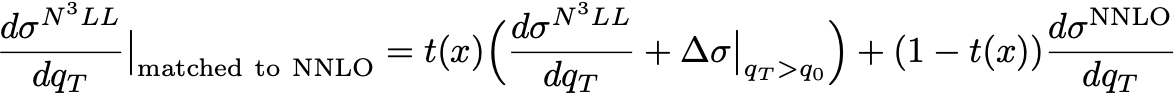
\includegraphics[width=0.9\textwidth]{./sections/Matching.png}
%\begin{equation}\label{eq:matchingmod}
%        \;
%	\left.\frac{\mathrm{d}\sigma^{\text{N$^3$LL}}}{\mathrm{d}q_T}\right|_{\text{matched to \NNLO{}}} 
%	=  t(x) \left( \frac{\mathrm{d}\sigma^{\text{N$^3$LL}}}{\mathrm{d}q_T} + 
%	\left.\Delta\sigma\right|_{q_T>q_0} \right)
%	+ (1-t(x)) \frac{\mathrm{d}\sigma^\NNLO{}}{\mathrm{d}q_T}\,
%\end{equation}

using a transition function $t(x)$. We have implemented a transition function $t$
with $x=q_T^2/Q^2$ that smoothly switches between 1 and 0 like a sigmoid function.

Following a choice in CuTe, we first define

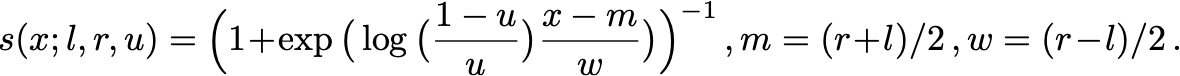
\includegraphics[width=0.9\textwidth]{./sections/sfunction.png}
%\begin{equation}
%s(x;l,r,u) = \left (1 + \exp\left(\log\left(\frac{1-u}{u}\right) \frac{x-m}{w}\right) \right )^{-1}\,,\quad
%m = (r+l)/2\,,\quad w = (r-l)/2\,.
%\end{equation}

The function $s(x)$, parametrized by $l,r,u$, is defined to be $s(l)=1-u$ and $s(r)=u$.
In terms of this sigmoid, our transition function $t(x; x^{\text{min}},x^{\text{max}},u)$, where 
$x=q_T^2/Q^2$, is then defined by
\begin{equation}\label{eq:transition}
	t(x; x^{\text{min}},x^{\text{max}},u) = \left\{\begin{array}{lr}
		1 , & \text{for } x < x^{\text{min}}\\
		\frac{s(x; x^{\text{min}}, x^{\text{max}},u)}
		     {s(x^{\text{min}}; x^{\text{min}}, x^{\text{max}},u)}, & 
		\text{otherwise}
	\end{array}\right\}\,.
\end{equation}
This ensures that below $x^{\text{min}}=(q_T^{\text{min}}/Q)^2$ only the naively matched result is 
used, and at
$x^{\text{max}}$
for small $u\ll1$ the transition function is approximately $u$. In practice it makes sense to set 
the transition
function to zero below a small threshold like $10^{-3}$ without a noticeable discontinuity.
This has the advantage that the deteriorating resummation and matching corrections do not impact 
the region of 
large $q_T$ at all.
Our example plotting routines use $x^{\text{min}}=0.001$, and $u=0.001$, and the parameter 
$x^{\text{max}}$ corresponds to the value of \texttt{transitionswitch} set in the input file. The 
transition function can be changed or completely replaced by just modifying the plotting routines. 
The following figure illustrates this transition function.

\begin{figure}[t!]
	\centering
	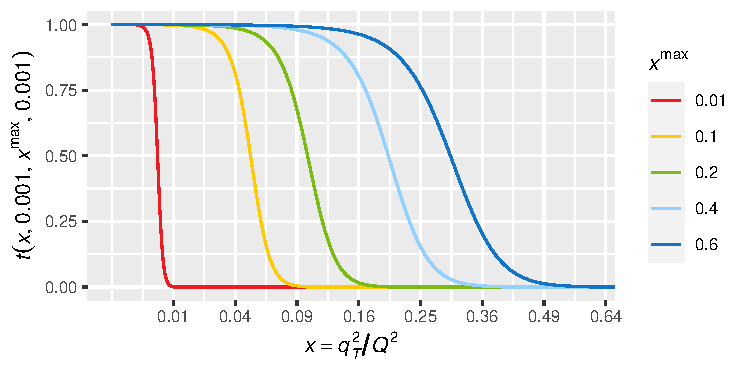
\includegraphics[width=0.8\textwidth]{transition.pdf}
	\caption{The transition function defined in eq.~\eqref{eq:transition} for different values of 
	the parameter $x^{\text{max}}$ which determines the position of the 
		transition. The $x$-axis is displayed on a square-root scale 
		to guide the eye on 
		the quadratic $q_T$-dependence.}
	\label{fig:transition}
\end{figure}

\midheading{Modifying the plotting routines and transition function.}
The plotting infrastructure has been completely rewritten for CuTe-MCFM, and we recommended to only 
use the new infrastructure
from this point on by setting \texttt{histogram\%newstyle = .true.} in
the input file. This is the default for the CuTe-MCFM example input files.

For the processes $W^\pm,Z,H$, $\gamma\gamma$, $Z\gamma$, $ZH$
and $W^\pm H$ we include predefined plotting routines that can be
adjusted. For example for $Z$ production the plotting routine is in the file
\texttt{src/User/nplotter\_Z\_new.f90}, and similarly for the other processes.
The routine \texttt{setup} defines all histograms with custom or uniform
binning and names. The
number of used histograms needs to be allocated in this routine. The
routine \texttt{book} is called for each phase space point. Through the
boolean variable \texttt{abovecut} it is known whether the routine is
called for ``boosted $q_T=0$'' (resummed part and fixed-order expansion of
resummed part) or for $q_T>0$ (fixed-order). All provided example input files
use the transition function as defined above, see also \href{https://arxiv.org/abs/2009.11437}{arXiv:2009.11437}.

The plotting routine returns the calculated observables in the
\texttt{vals} array, and Vegas weights in \texttt{wts}. The transition
function is implemented by reweighting the original Vegas weights with
the output of the transition function. To disable the transition
function, one sets \texttt{trans} to $1$ before filling the \texttt{wts}
array.

Apart from modifying a default set of kinematical cuts in the input
file, cuts can also be set in the file
\texttt{src/User/gencuts\_user.f90} in a fully flexible way based on the
event's four momenta. Some commented out examples are included there.




\newpage

\topheading{Jet-vetoed cross sections}
\label{jetvetosec}
The jet veto scale $p_T^{{\rm veto}}$ can induce large logarithms
if it is smaller than the hard process scale $Q$, which then mandates
resummation.
We consider processes where jets have been defined using
sequential recombination jet algorithms \cite{Salam:2010nqg} with distance measure
\begin{equation}\label{jetdef}
        d_{ij} = \mbox{min}(k_{Ti}^{2n},k_{Tj}^{2n})\,
        \frac{\Delta y_{ij}^2+\Delta\phi_{ij}^2}{R^2} \,, \qquad
        d_{iB} = k_{Ti}^{2n} \,,
\end{equation}
where the choice $n=-1$ is the anti-$k_T$ algorithm \cite{Cacciari:2008gp},
$n=0$ is the Cambridge-Aachen algorithm \cite{Dokshitzer:1997in,Wobisch:1998wt},
and $n=1$ is the $k_T$ algorithm \cite{Catani:1993hr,Ellis:1993tq}.
$k_{Ti}$ denotes the transverse momentum of (pseudo-)particle $i$ with respect to the beam
direction,
and $\Delta y_{ij}$ and $\Delta\phi_{ij}$ are the rapidity and azimuthal angle differences of
(pseudo-)particles $i$ and $j$.

\midheading{Benchmark results for jet-vetoed cross sections}
Results for benchmark cross sections for a variety of single-boson processes
taken from ref.~\cite{CENS} are shown in  Tables~\ref{table:jetveto_H}--\ref{table:jetveto_Z}
and for diboson processes in
Tables~\ref{table:jetveto_WW}--\ref{table:jetveto_ZZ}.
The input files are linked in the tables.
The uncertainties indicated in these tables
represent the numerical integration (Monte Carlo) uncertainty.

\renewcommand{\arraystretch}{1.05}
\begin{table}
\begin{tabular}{llll}
\hline
Final state & input file & contribution & cross section \\
\hline
$H$ & \href{\mcfmprocs/Files119/jetveto/veto30nlo.ini}{\texttt{H/veto30nlo.ini}}       & NLO                 &  $26.23 \pm 0.01$ pb   \\
    & \href{\mcfmprocs/Files119/jetveto/veto30nnlo.ini}{\texttt{H/veto30nnlo.ini}}     & NNLO                &  $28.97 \pm 0.09$ pb \\
    & \href{\mcfmprocs/Files119/jetveto/veto30nnll.ini}{\texttt{H/veto30nnll.ini}}     & NNLL                &  $24.89 \pm 0.01$ pb \\
    & \href{\mcfmprocs/Files119/jetveto/veto30n3ll.ini}{\texttt{H/veto30n3ll.ini}}     & N$^3$LL$_p$         &  $24.29 \pm 0.01$ pb \\
    & \href{\mcfmprocs/Files119/jetveto/veto30nlomc.ini}{\texttt{H/veto30nlomc.ini}}   & NLO+NNLL MC         &  $2.25 \pm 0.01$ pb \\
    & \href{\mcfmprocs/Files119/jetveto/veto30nnlomc.ini}{\texttt{H/veto30nnlomc.ini}} & NNLO+N$^3$LL$_p$ MC &  $3.89 \pm 0.19$ pb \\[2pt]
\hline
\end{tabular}
\caption{Benchmark results for jet-vetoed Higgs cross sections.}
\label{table:jetveto_H}
\end{table}
\renewcommand{\arraystretch}{1.0}

\renewcommand{\arraystretch}{1.05}
\begin{table}
\begin{tabular}{llll}
\hline
Final state & input file & contribution & cross section \\
\hline
$W^+$                                                                                
& \href{\mcfmprocs/Files1/jetveto/vetowp30nlo.ini}{\texttt{W/vetowp30nlo.ini}}        & NLO                 & $3.048 \pm 0.001$ nb \\
& \href{\mcfmprocs/Files1/jetveto/vetowp30nnlo.ini}{\texttt{W/vetowp30nnlo.ini}}      & NNLO                & $2.81 \pm 0.003$ nb \\
& \href{\mcfmprocs/Files1/jetveto/vetowp30nnll.ini}{\texttt{W/vetowp30nnll.ini}}      & NNLL                & $2.517 \pm 0.002$ nb \\
& \href{\mcfmprocs/Files1/jetveto/vetowp30n3ll.ini}{\texttt{W/vetowp30n3ll.ini}}      & N$^3$LL$_p$         & $2.250 \pm 0.002$ nb \\
& \href{\mcfmprocs/Files1/jetveto/vetowp30nlomc.ini}{\texttt{W/vetowp30nlomc.ini}}    & NLO+NNLL MC         & $0.561 \pm 0.006$ nb \\
& \href{\mcfmprocs/Files1/jetveto/vetowp30nnlomc.ini}{\texttt{W/vetowp30nnlomc.ini}}  & NNLO+N$^3$LL$_p$ MC & $0.57 \pm 0.02$ nb \\[2pt]
\hline                                                                               
$W^-$                                                                                
& \href{\mcfmprocs/Files6/jetveto/vetowm30nlo.ini}{\texttt{W/vetowm30nlo.ini}}        & NLO                 & $2.101 \pm 0.001$ nb \\
& \href{\mcfmprocs/Files6/jetveto/vetowm30nnlo.ini}{\texttt{W/vetowm30nnlo.ini}}      & NNLO                & $1.979 \pm 0.002$ nb \\
& \href{\mcfmprocs/Files6/jetveto/vetowm30nnll.ini}{\texttt{W/vetowm30nnll.ini}}      & NNLL                & $1.796 \pm 0.002$ nb \\
& \href{\mcfmprocs/Files6/jetveto/vetowm30n3ll.ini}{\texttt{W/vetowm30n3ll.ini}}      & N$^3$LL$_p$         & $1.600 \pm 0.001$ nb \\
& \href{\mcfmprocs/Files6/jetveto/vetowm30nlomc.ini}{\texttt{W/vetowm30nlomc.ini}}    & NLO+NNLL MC         & $0.327 \pm 0.003$ nb \\
& \href{\mcfmprocs/Files6/jetveto/vetowm30nnlomc.ini}{\texttt{W/vetowm30nnlomc.ini}}  & NNLO+N$^3$LL$_p$ MC & $0.33 \pm 0.01$ nb \\[2pt]
\hline
\end{tabular}
\caption{Benchmark results for jet-vetoed $W^\pm$ cross sections.}
\label{table:jetveto_W}
\end{table}
\renewcommand{\arraystretch}{1.0}

\renewcommand{\arraystretch}{1.05}
\begin{table}
\begin{tabular}{llll}
\hline
Final state & input file & contribution & cross section \\
\hline
$Z$ & \href{\mcfmprocs/Files31/jetveto/veto30nlo.ini}{\texttt{Z/veto30nlo.ini}}        & NLO                 & $668 \pm 1$ pb \\
    & \href{\mcfmprocs/Files31/jetveto/veto30nnlo.ini}{\texttt{Z/veto30nnlo.ini}}      & NNLO                & $628 \pm 2$ pb \\
    & \href{\mcfmprocs/Files31/jetveto/veto30nnll.ini}{\texttt{Z/veto30nnll.ini}}      & NNLL                & $676 \pm 2$ pb \\
    & \href{\mcfmprocs/Files31/jetveto/veto30n3ll.ini}{\texttt{Z/veto30n3ll.ini}}      & N$^3$LL$_p$         & $596 \pm 2$ pb \\
    & \href{\mcfmprocs/Files31/jetveto/veto30nlomc.ini}{\texttt{Z/veto30nlomc.ini}}    & NLO+NNLL MC         & $-11 \pm 1$ pb \\
    & \href{\mcfmprocs/Files31/jetveto/veto30nnlomc.ini}{\texttt{Z/veto30nnlomc.ini}}  & NNLO+N$^3$LL$_p$ MC & $-7.7 \pm 0.7$ pb \\[2pt]
\hline
\end{tabular}
\caption{Benchmark results for jet-vetoed $Z$ cross sections.}
\label{table:jetveto_Z}
\end{table}
\renewcommand{\arraystretch}{1.0}

\renewcommand{\arraystretch}{1.05}
\begin{table}
\begin{tabular}{llll}
\hline
Final state & input file & contribution & cross section \\
\hline
$WW$
     & \href{\mcfmprocs/Files61/jetveto/veto30nlo.ini}{\texttt{WW/veto30nlo.ini}}       & NLO                 & $234.0 \pm 0.2$ fb \\
     & \href{\mcfmprocs/Files61/jetveto/veto30nnlo.ini}{\texttt{WW/veto30nnlo.ini}}      & NNLO                & $242.7 \pm 0.4$ fb \\
     & \href{\mcfmprocs/Files61/jetveto/veto30nnll.ini}{\texttt{WW/veto30nnll.ini}}      & NNLL                & $204.7 \pm 0.2$ fb \\
     & \href{\mcfmprocs/Files61/jetveto/veto30n3ll.ini}{\texttt{WW/veto30n3ll.ini}}      & N$^3$LL$_p$         & $205.2 \pm 0.2$ fb \\
     & \href{\mcfmprocs/Files61/jetveto/veto30nlomc.ini}{\texttt{WW/veto30nlomc.ini}}    & NLO+NNLL MC         & $25.8 \pm 0.9$ fb \\
     & \href{\mcfmprocs/Files61/jetveto/veto30nnlomc.ini}{\texttt{WW/veto30nnlomc.ini}}  & NNLO+N$^3$LL$_p$ MC & $19.8 \pm 0.6$ fb \\[2pt]
\hline
\end{tabular}
\caption{Benchmark results for jet-vetoed $W^+W^-$ cross sections.}
\label{table:jetveto_WW}
\end{table}
\renewcommand{\arraystretch}{1.0}

\renewcommand{\arraystretch}{1.05}
\begin{table}
\begin{tabular}{llll}
\hline
Final state & input file & contribution & cross section \\
\hline
\hline
$W^+Z$
& \href{\mcfmprocs/Files71/jetveto/atlas/vetowp25nlo.ini}{\texttt{WZ-atlas/vetowp25nlo.ini}}        & NLO                 & $20.11 \pm 0.01$ fb \\
& \href{\mcfmprocs/Files71/jetveto/atlas/vetowp25nnlo.ini}{\texttt{WZ-atlas/vetowp25nnlo.ini}}      & NNLO                & $19.14 \pm 0.02$ fb \\
& \href{\mcfmprocs/Files71/jetveto/atlas/vetowp25nnll.ini}{\texttt{WZ-atlas/vetowp25nnll.ini}}      & NNLL                & $18.87 \pm 0.01$ fb \\
& \href{\mcfmprocs/Files71/jetveto/atlas/vetowp25n3ll.ini}{\texttt{WZ-atlas/vetowp25n3ll.ini}}      & N$^3$LL$_p$         & $17.72 \pm 0.01$ fb \\
& \href{\mcfmprocs/Files71/jetveto/atlas/vetowp25nlomc.ini}{\texttt{WZ-atlas/vetowp25nlomc.ini}}    & NLO+NNLL MC         & $0.17 \pm 0.06$ fb \\
& \href{\mcfmprocs/Files71/jetveto/atlas/vetowp25nnlomc.ini}{\texttt{WZ-atlas/vetowp25nnlomc.ini}}  & NNLO+N$^3$LL$_p$ MC & $0.07 \pm 0.01$ fb \\[2pt]
\hline
$W^-Z$
& \href{\mcfmprocs/Files76/jetveto/atlas/vetowm25nlo.ini}{\texttt{WZ-atlas/vetowm25nlo.ini}}        & NLO                 & $13.54 \pm 0.01$ fb \\
& \href{\mcfmprocs/Files76/jetveto/atlas/vetowm25nnlo.ini}{\texttt{WZ-atlas/vetowm25nnlo.ini}}      & NNLO                & $12.82 \pm 0.01$ fb \\
& \href{\mcfmprocs/Files76/jetveto/atlas/vetowm25nnll.ini}{\texttt{WZ-atlas/vetowm25nnll.ini}}      & NNLL                & $12.66 \pm 0.01$ fb \\
& \href{\mcfmprocs/Files76/jetveto/atlas/vetowm25n3ll.ini}{\texttt{WZ-atlas/vetowm25n3ll.ini}}      & N$^3$LL$_p$         & $11.77 \pm 0.01$ fb \\
& \href{\mcfmprocs/Files76/jetveto/atlas/vetowm25nlomc.ini}{\texttt{WZ-atlas/vetowm25nlomc.ini}}    & NLO+NNLL MC         & $0.21 \pm 0.04$ fb \\
& \href{\mcfmprocs/Files76/jetveto/atlas/vetowm25nnlomc.ini}{\texttt{WZ-atlas/vetowm25nnlomc.ini}}  & NNLO+N$^3$LL$_p$ MC & $0.12 \pm 0.01$ fb \\[2pt]
\end{tabular}
\caption{Benchmark results for jet-vetoed $WZ$ cross sections.}
\label{table:jetveto_WZ-atlas}
\end{table}
\renewcommand{\arraystretch}{1.0}

\renewcommand{\arraystretch}{1.05}
\begin{table}
\begin{tabular}{llll}
\hline
Final state & input file & contribution & cross section \\
\hline
$ZZ$
& \href{\mcfmprocs/Files81/jetveto/veto30nlo.ini}{\texttt{ZZ/veto30nlo.ini}}        & NLO                 & $12.17 \pm 0.01$ fb \\
& \href{\mcfmprocs/Files81/jetveto/veto30nnlo.ini}{\texttt{ZZ/veto30nnlo.ini}}      & NNLO                & $12.88 \pm 0.01$ fb \\
& \href{\mcfmprocs/Files81/jetveto/veto30nnll.ini}{\texttt{ZZ/veto30nnll.ini}}      & NNLL                & $11.90 \pm 0.01$ fb \\
& \href{\mcfmprocs/Files81/jetveto/veto30n3ll.ini}{\texttt{ZZ/veto30n3ll.ini}}      & N$^3$LL$_p$         & $11.85 \pm 0.01$ fb \\
& \href{\mcfmprocs/Files81/jetveto/veto30nlomc.ini}{\texttt{ZZ/veto30nlomc.ini}}    & NLO+NNLL MC         & $-0.22 \pm 0.01$ fb \\
& \href{\mcfmprocs/Files81/jetveto/veto30nnlomc.ini}{\texttt{ZZ/veto30nnlomc.ini}}  & NNLO+N$^3$LL$_p$ MC & $-0.17 \pm 0.01$ fb \\[2pt]
\hline
\end{tabular}
\caption{Benchmark results for jet-vetoed $ZZ$ cross sections.}
\label{table:jetveto_ZZ}
\end{table}
\renewcommand{\arraystretch}{1.0}


\newpage

\topheading{Z production at N$^3$LO and N$^4$LL}
\label{n3losec}

Based on \href{https://arxiv.org/abs/2207.07056}{arXiv:2207.07056} (Neumann, Campbell '22).

This page describes how to obtain Z-boson predictions at the level of up
to N$^4$LL+N$^3$LO and at a fixed order of up to N$^3$LO. The
highest order predictions are then are at the level of $\alpha_s^3$ up
to missing N$^3$LO PDFs, which both affect the logarithmic accuracy
and the fixed-order accuracy.

\textbf{Warning}: Please note that predictions at the level of
$\alpha_s^3$ are computationally very expensive due to the Z+jet NNLO
matching corrections calculated with a small (5 GeV) cutoff. Our
production plots typically run on 128 NERSC Perlmutter nodes for 12
hours, about 100k CPU hours. If you do not have these resources and are
mostly interested in the region of small $q_T$ (less than about 40 GeV), the
matching to fixed order can be performed at the level of $\alpha_s^2$.
This changes results by about 10\% above 40 GeV (missing
$\alpha_s^3$/Z+jet NNLO corrections at large $q_T$), but typically
just at the level of 2\% below 30 GeV, depending on cuts.

For $Z$ production one can start with the input file
\texttt{Bin/input\_Z.ini} that has a set of default cuts for $Z$
production, i.e.~a mass window of the lepton pair around $m_Z$
(\texttt{m34min} and \texttt{m34max} are set), and lepton minimum
transverse momenta (\texttt{ptleptmin} and \texttt{ptlept2min}, both the
same, i.e.~symmetric cuts).

After choosing a set of PDFs (\texttt{lhapdf\%lhapdfset}), beamfunctions
grids should be pre-generated by running MCFM with
\texttt{resummation\%makegrid=.true.}.


\midheading{N$^4$LL + matching at $\alpha_s^2$ fixed-order (NLO~$Z$+jet)}

The fully matched result consists of the purely resummed part, the
fixed-order Z+jet calculation and the fixed-order expansion of the
resummation to remove overlap. At N$^3$LL$^\prime$+NNLO these three
parts can be computed together automatically with
\texttt{general\%part=resNNLOp}, or with \texttt{general\%part=resNNLO}
at N$^3$LL+NNLO (\texttt{general\%part=resNLO} at NNLL+NLO). At the
level of N$^4$LL+N$^3$LO the matching is with NNLO Z+jet predictions
and, due to the computational requirements, these three parts are kept
separate and have to be assembled manually.


\bottomheading{Purely resummed N$^4$LL}

The purely resummed N$^4$LL part can be obtained by running with
\texttt{part\ =\ resonlyN3LO}. Similarly the N$^3$LL resummation is
obtained with \texttt{part\ =\ resonlyNNLO} and N$^3$LL$^\prime$
with \texttt{part\ =\ resonlyNNLOp} (see overview of configuration
options). Scale variation of hard, low and rapidity scale can be enabled
with \texttt{scales\%doscalevar\ =\ .true.}.

The resummation part will be cut off at large transverse momenta through
a transition function defined in the plotting routine. We recommend to
use the default transition function with a parameter $(q_T^2/Q^2)=0.4$
or $0.6$. The default plotting routine generates histograms with both
choices that allows for estimating a matching uncertainty.

Since the resummation becomes also invalid and numerically unstable for
$q_T>m_Z$, we select the resummation integration range between $0$
and $80$ GeV with \texttt{resummation\%res\_range=0\ 80}.



\bottomheading{Fixed-order expansion of the resummed result}

The fixed-order expansion of the resummed result (removing overlap with
fixed-order Z+jet at NLO) (in the following called resexp) can be
obtained by running \texttt{part\ =\ resexpNNLO}. We recommend a lower
cutoff of 1 GeV, setting \texttt{resexp\_range\ =\ 1.0\ 80.0} in the
\texttt{resummation} section.

This part makes use of the transition function to ensure that this part
is turned off at large $q_T$. Therefore the range is also limited to
80 GeV.



\bottomheading{Fixed-order Z+jet at NLO}

The fixed-order $\alpha_s^2$ corrections (in the following called
resabove) can be obtained by running \texttt{part\ =\ resaboveNNLO}. We
recommend a cutoff of 1 GeV, setting \texttt{fo\_cutoff\ =\ 1.0} in the
\texttt{resummation} section. This cutoff disables matching corrections
below 1 GeV and must agree with the lower value of
\texttt{resexp\_range}.


\bottomheading{Combination and scale uncertainties}

After running all three parts separately, the generated histograms can
be added manually in a plotting program. The matching corrections
consist of fixed-order result + fixed-order expansion of the resummed
result. At $\alpha_s^2$ a manual combination should agree with an
automatic combination through \texttt{part\ =\ resNNLO}, for example.

To obtain uncertainties from scale variation the following procedure
should be followed. The scales in the matching corrections must match,
i.e.~resexp\_scalevar\_01 should be added to resabove\_scalevar\_01, and
resexp\_scalevar\_02 should be added to resexp\_scalevar\_02. Note that
the scale variation histograms only give the difference to the central
value. So the minimum of the scale varied matching corrections consist
of:

\begin{verbatim}
	min(resabove + resabove_scalevar_01 + resexp + resexp_scalevar_01,
	resabove + resabove_scalevar_02 + resexp + resexp_scalevar_02)
\end{verbatim}

Similarly the maximum can be taken, both giving an envelope of
uncertainties. Note that in the resummation and its fixed-order
expansion we have not decoupled the scale in the PDFs from other scales.
Therefore when combining resexp with resabove, only the simultaneous
variation of factorization scale and renormalization scale upwards and
downwards can be used for the scale variation, corresponding to "\_01"
and "\_02".

Finally the scalevar\_maximum and scalevar\_minimum histograms of the
purely resummed result should be considered as an additional envelope.
For this part the envelope of all scale variations is taken. The
variation of the rapidity scale plays an important role and can be
enabled by setting \texttt{scalevar\_rapidity\ =\ .true.} in the
\texttt{{[}resummation{]}} section. It gives two important additional
variations to the 2, 6, or 8-point variation of hard and resummation
scale in the resummed part.

\midheading{Adding $\alpha_s^3$ matching corrections (Z+jet NNLO coefficient)}

To obtain the matching corrections at $\alpha_s^3$ we compute just the
$\alpha_s^3$ \emph{coefficient} and add it to the previously obtained
lower order results.


\bottomheading{Fixed-order Z+jet NNLO coefficient}

To obtain the fixed-order $\alpha_s^3$ corrections please run with
\texttt{part\ =\ resaboveN3LO}. We recommend a matching cutoff of 5 GeV,
setting \texttt{fo\_cutoff\ =\ 5.0} in the \texttt{resummation} section
and consequently a jettiness cutoff of \texttt{taucut=0.08} in the
\texttt{nnlo} section. It is possible to run with a larger
\texttt{fo\_cutoff} keeping the same \texttt{taucut} value, but either a
smaller \texttt{fo\_cutoff} or a larger \texttt{taucut} value will
require a new validation of results.



\bottomheading{Fixed-order Z+jet NNLO coefficient}

To obtain the fixed-order $\alpha_s^3$ corrections please run the
$Z$+jet process (\texttt{nproc=41}) with \texttt{part=nnlocoeff} in
the \texttt{{[}general{]}} section with a fixed $q_T$ cutoff, i.e.~by
setting \texttt{pt34min\ =\ 5.0} in the \texttt{{[}masscuts{]}} section.
The Z+jet calculation is based on jettiness slicing, which requires a
jettiness cutoff. For a $q_T$ cutoff of 5 GeV (for resummation this is
the matching-corrections cutoff) we recommend a jettiness cutoff of
\texttt{taucut=0.08} in the \texttt{{[}nnlo{]}} section. It is possible
to run with a larger $q_T$ cutoff, keeping the same \texttt{taucut}
value, but either a smaller $q_T$ cutoff or a larger \texttt{taucut}
value will require a new validation of results. See
\href{https://arxiv.org/abs/2207.07056}{arXiv:2207.07056} for technical
details.


\bottomheading{$\alpha_s^3$ fixed-order expansion coefficient of the resummed result}

The $\alpha_s^3$ fixed-order expansion coefficient of the resummed
result (removing overlap with fixed-order Z+jet at NNLO) can be obtained
by running \texttt{part\ =\ resexpN3LO}. \textbf{\emph{NOTE}} that this
only returns the N$^3$LO expansion \textbf{\emph{coefficient}}, to
match with the fixed-order \texttt{nnlocoeff} part. Similarly, to match
with the fixed-order part, we recommend a cutoff of 5 GeV, setting
\texttt{resexp\_range\ =\ 5.0\ 80.0} in the \texttt{resummation}
section.

\bottomheading{Combination}

Similary to the lower order, the matching corrections $\alpha_s^3$
coefficient can be added to lower order $\alpha_s^2$ results.

\midheading{Fixed order	N$^3$LO}

To compute fixed-order N$^3$LO cross-sections with $q_T$
subtractions one needs to calculate the fixed-order Z+jet NNLO
coefficient with a $q_T$ cutoff, as outlined above. The below-cut
contribution can be obtained via \texttt{part=n3locoeff} in the
\texttt{{[}general{]}} section for $Z$ production,
i.e.~\texttt{nproc=31}, where the \texttt{qtcut} value in the
\texttt{{[}nnlo{]}} section has to match the \texttt{pt34min} value
chosen for the Z+jet NNLO calculation.

We recommend to calculate the fixed-order NNLO coefficient first, as it
is instructional to understand the procedure at N$^3$LO. This proceeds
by combining NLO Z+jet result with a \texttt{pt34min} value with the
\texttt{part=nnloVVcoeff} part (below-cut at NNLO), where \texttt{qtcut}
has to be set to match the \texttt{pt34min} value. The result of this
manual procedure must agree with the automatic calculation,
i.e.~calculating Z with \texttt{part=nnlo} or \texttt{part=nnlocoeff}.
Please pay particular attention to the difference of calculating the
NNLO ($\alpha_s^2$) and N$^3$LO ($\alpha_s^3$) coefficients and
the full result.


\hypertarget{c-interface}{%
\section{C++ interface to One-Loop Matrix Elements}\label{c-interface}}

Since version 10.1, MCFM offers a dedicated C++ interface to access its
analytic one-loop amplitudes. Please cite ref.~\cite{Campbell:2021vlt} in
addition to the main MCFM references when using the C++ interface.

\hypertarget{available-processes}{%
\subsection{Available Processes}\label{available-processes}}

The following Standard-Model processes are available:

\begin{longtable}[]{@{}lll@{}}
\toprule
Process & Order EW & Order QCD \\
\midrule
\endhead
\(pp\to \ell^+\ell^-\) & 2 & 1 \\
\(pp\to \ell^+\ell^- j\) & 2 & 2 \\
\(pp\to \ell^+\ell^- j j\) & 2 & 3 \\
& & \\
\(pp\to \ell^\pm\nu_\ell\) & 2 & 1 \\
\(pp\to \ell^\pm\nu_\ell j\) & 2 & 2 \\
\(pp\to \ell^\pm\nu_\ell j j\) & 2 & 3 \\
& & \\
\(pp\to h\) & 1 & 2 \\
\(pp\to h j\) & 1 & 3 \\
\(pp\to h j j\) & 1 & 4 \\
& & \\
\(pp\to h h\) & 2 & 2 \\
& & \\
\(pp\to \ell^+\ell^- h\) & 3 & 1 \\
\(pp\to \ell^+\ell^- h j\) & 3 & 2 \\
& & \\
\(pp\to \ell^\pm\nu_\ell h\) & 3 & 1 \\
\(pp\to \ell^\pm\nu_\ell h j\) & 3 & 2 \\
& & \\
\(pp\to \gamma j\) & 1 & 2 \\
\(pp\to \gamma j j\) & 1 & 3 \\
& & \\
\(pp\to \gamma \gamma\) & 2 & 1 \\
\(gg\to \gamma \gamma\) & 2 & 1 \\
\(pp\to \gamma \gamma j\) & 2 & 2 \\
& & \\
\(pp\to \gamma \gamma \gamma\) & 3 & 1 \\
& & \\
\(pp\to \gamma \gamma \gamma \gamma\) & 4 & 1 \\
& & \\
\(pp\to \ell^+\ell^-\gamma\) & 3 & 1 \\
\(pp\to \ell^\pm\nu_\ell\gamma\) & 3 & 1 \\
\(pp\to \nu_\ell\bar\nu_\ell\gamma\) & 3 & 1 \\
& & \\
\(pp\to \ell^+\ell^{\prime-}\nu_\ell\bar\nu_{\ell'}\) & 4 & 1 \\
& & \\
\(pp\to \ell^+\ell^-\nu_{\ell'}\bar\nu_{\ell'}\) & 4 & 1 \\
\(pp\to \ell^+\ell^-\ell^{\prime+}\ell^{\prime-}\) & 4 & 1 \\
\(pp\to \ell^+\ell^-\ell^+\ell^-\) & 4 & 1 \\
& & \\
\(pp\to \ell^+\ell^-\ell^{\prime\pm}\nu_{\ell'}\) & 4 & 1 \\
\(pp\to \ell^\pm\nu_\ell\nu_{\ell'}\bar\nu_{\ell'}\) & 4 & 1 \\
& & \\
\(pp\to t \bar t\) & 0 & 3 \\
& & \\
\(pp\to j j\) & 0 & 3 \\
\bottomrule
\end{longtable}

In addition, the following HEFT processes are available (requires
model=heft):

\begin{longtable}[]{@{}lll@{}}
\toprule
Process & Order EW & Order QCD \\
\midrule
\endhead
\(pp\to h\) & 1 & 2 \\
\(pp\to h j\) & 1 & 3 \\
\(pp\to h j j\) & 1 & 4 \\
\bottomrule
\end{longtable}

All processes are crossing invariant.

Further processes as per the
{\lstinline!process list <processlist>!} may be
implemented in the future. Please contact the authors if interested in a
specific process.

\hypertarget{installation}{%
\subsection{Installation}\label{installation}}

To use the C++ interface, please enable compiling MCFM as a library by
adding the {\lstinline!-DWITH_LIBRARY!} flag

\begin{lstlisting}
cmake .. -DWITH_LIBRARY
\end{lstlisting}

This will create a shared library {\lstinline!libMCFM.so!}
in the {\lstinline!lib/!} directory.

\hypertarget{usage}{%
\subsection{Usage}\label{usage}}

Examples showing the basic usage of the interface and how to fill the
complete list of parameters with default values are given in
{\lstinline!src/BLHA/text.cxx!} and
{\lstinline!src/BLHA/params.cxx!}, respectively.

The MCFM C++ interface is constructed as a C++ class

\begin{lstlisting}[language={C++}]
CXX_Interface mcfm;
\end{lstlisting}

included in the header

\begin{lstlisting}[language={C++}]
#include "MCFM/CXX_Interface.h"
\end{lstlisting}

It must be initialized on a \(\texttt{std::map}\) of
\(\texttt{std::string}\), containing all (standard-model) parameters

\begin{lstlisting}[language={C++}]
bool CXX_Interface::Initialize(std::map<std::string,std::string>& parameters);
\end{lstlisting}

Prior to use, each process has to be initialized in the interface

\begin{lstlisting}[language={C++}]
int CXX_Interface::InitializeProcess(const Process_Info &pi);
\end{lstlisting}

which takes a {\lstinline!Process\_Info!} object as input,
which in turn contains the defining parameters of a given process,
i.e.~the PDG IDs, number of incoming particles, and QCD and EW coupling
orders

\begin{lstlisting}[language={C++}]
Process_Info(const std::vector<int> &ids, const int nin,const int oqcd, const int oew);
\end{lstlisting}

Phase space points are defined using the
{\lstinline!FourVec!} struct, which represents four-vectors
in the ordering \((E, p_x, p_y, p_z)\)

\begin{lstlisting}[language={C++}]
FourVec(double e, double px, double py, double pz);
\end{lstlisting}

Given a list of four-vectors in this format, one-loop matrix elements
can be calculated either using the process ID returned by the
{\lstinline!InitializeProcess!} method

\begin{lstlisting}[language={C++}]
void CXX_Interface::Calc(int procID,const std::vector<FourVec> &p, int oqcd);
\end{lstlisting}

or using a {\lstinline!Process\_Info!} struct:

\begin{lstlisting}[language={C++}]
void CXX_Interface::Calc(const Process_Info &pi,const std::vector<FourVec> &p,int oqcd);
\end{lstlisting}

In the same way, the result of this calculation can be accessed either
via the process ID

\begin{lstlisting}[language={C++}]
const std::vector<double>& CXX_Interface::GetResult(int procID);
\end{lstlisting}

or using the {\lstinline!Process\_Info!} struct:

\begin{lstlisting}[language={C++}]
const std::vector<double> &CXX_Interface::GetResult(const Process_Info &pi)
\end{lstlisting}

The result is returned as a list of Laurent series coefficients in the
format
\begin{equation*}
(\mathcal{O}(\varepsilon^0), \mathcal{O}(\varepsilon^{-1}), \mathcal{O}(\varepsilon^{-2}), \mathrm{Born})
\;.
\end{equation*}
However, by default only the \(\mathcal{O}(\varepsilon^0)\) coefficient,
i.e.~the finite part, is returned.

The calculation of the pole terms and the Born can be enabled by setting
the following switch to {\lstinline!1!}

\begin{lstlisting}[language={C++}]
void CXX_Interface::SetPoleCheck(int check);
\end{lstlisting}

\hypertarget{tests}{%
\subsection{Tests}\label{tests}}

A set of programs to test MCFM's amplitudes against
\href{https://openloops.hepforge.org}{OpenLoops},
\href{https://recola.gitlab.io/recola2/}{Recola}, and
\href{http://madgraph.phys.ucl.ac.be}{MadLoop} can be compiled. For
example to compile the OpenLoops test program an additional OpenLoops
directory {\lstinline!-DOLDIR=$HOME/OpenLoops!} must be
specified that contains the header files in the
{\lstinline!include!} subdirectory. For Recola and MadLoops
the variables {\lstinline!RCLDIR!} and
{\lstinline!MLDIR!} must be specified, respectively.



\topheading{Notes on specific processes}

\label{sec:specific}

The processes described in the file {\tt process.DAT} include
appropriate boson decays when the parameter {\tt removebr} is set to
{\tt .false.}. In many cases a more simple calculation can be
performed by setting this parameter to {\tt .true.}, in which case
these decays are not performed.  Technically the full calculation
including the decays is still performed but cuts are not performed on
the decay products and the branching ratio is divided out, thus
yielding the cross section before decay.  In the notes below we
indicate the simpler processes thus obtained. When running in this
mode, the parameter {\tt zerowidth} should be set to {\tt .true.} for
consistency. However in certain circumstances, for the sake of
comparison, it may be useful to run with it set to {\tt .false.}.

\midheading{$W$-boson production, processes 1,6}
\label{subsec:wboson}

These processes represent the production of a $W$ boson which subsequently
decays leptonically. 
This process can be calculated at LO, NLO, and NNLO.
NLO calculations can be performed by dipole subtraction, 
zero-jettiness slicing and $q_T$-slicing.
NNLO calculations can be performed by  zero-jettiness slicing and $q_T$-slicing.

When {\tt removebr} is true, the $W$ boson does not decay.

\midheading{EW corrections to $W$-boson production, processes 2,7}
\label{subsec:wbosonew}

These processes compute the electroweak corrections to the production of
a $W$ boson which subsequently decays leptonically.
The electron is taken to be massless.
The electroweak corrections involve both real and virtual corrections.
If particle 5 is present it is a photon.
The calculation must be performed at NLO, i.e.~{\tt part=nlo}.

\midheading{Photon-induced corrections to $W$-boson production, processes 3,8}
\label{subsec:wbosonphoton}

These processes compute the production of
a $W$ boson, (which subsequently decays leptonically),
through the reaction $q + \gamma \to e + \nu + q$.
The calculation must be performed at NLO.
Since the reaction has an initial
photon, it is important to have an accurate parton distribution function for
the photon in the proton, e.g. LUXqed17\_plus\_PDF4LHC15\_nnlo\_30.

\midheading{$W+$~jet production, processes 11,16}
\label{subsec:w1jet}
This process is calculable at leading LO and next-to-leading order NLO.
These processes represent the production of a $W$ boson which subsequently
decays leptonically, in association with a single jet.
When {\tt removebr} is true, the $W$ boson does not decay.

\midheading{$W+b$ production, processes 12,17}
\label{subsec:wb}

These processes represent the production of a $W$ boson which
subsequently decays leptonically, in association with a single bottom
quark, exploiting the weak transitions $c \to b$ and $u \to b$.
This is produced at leading order by an initial state which
contains a charm quark (or the CKM  suppressed $u$ quark) and a
gluon, e.g
$ c(-p_1)+g(p_2) \to W^+(\to \nu(p_3)+e^+(p_4))+b(p_5)$
and
$ u(-p_1)+g(p_2) \to W^+(\to \nu(p_3)+e^+(p_4))+b(p_5)$
or the charge conjugate processes for $W^{-}$.
This process is somewhat analogous to single top production.

The effect of the bottom quark mass is included throughout the calculation.  
For this case the CKM matrix elements $V_{cb}$ and $V_{ub}$,
(if they are equal to zero in the input data file, {\tt mdata.f})
are set equal to $0.041$ and $0.00347$ respectively. 
Otherwise the non-zero values specified in {\tt mdata.f} are used. 
The calculation of this process may
be performed at LO and NLO.

When {\tt removebr} is true, the $W$ boson does not decay.


\midheading{$W+c$ production, processes 13,18}
\label{subsec:wc}

These processes represent the production of a $W$ boson which
subsequently decays leptonically, in association with a charm
quark. 
This is produced at leading order by an initial state which
contains a strange anti-quark (or Cabibbo suppressed $d$ anti-quark) and a
gluon, e.g
$ \bar{d}(-p_1)+g(p_2) \to W^+(\to \nu(p_3)+e^+(p_4))+\bar{c}(p_5)$
and
$ \bar{u}(-p_1)+g(p_2) \to W^+(\to \nu(p_3)+e^+(p_4))+\bar{c}(p_5)$
or the charge conjugate process for $W^{-}$.
This process is somewhat analogous to single top production.

The effect of the charm quark mass is included throughout the
calculation.  The calculation of this process may
be performed both at LO and NLO.

When {\tt removebr} is true, the $W$ boson does not decay.

\midheading{$W+c$ production ($m_c=0$), processes 14,19}
\label{subsec:wcmassless}

These processes are identical to {\tt 13} and {\tt 18} except for the fact
that the charm quark mass is neglected. The calculation can currently be
performed at LO only.

\midheading{$W+b{\bar b}$ production, processes 20,25}
\label{subsec:wbb}

This process is calculable at leading LO and next-to-leading order NLO.
These processes represent the production of a $W$ boson which subsequently
decays leptonically, in association with a $b{\bar b}$ pair. The effect of
the bottom quark mass is included throughout the calculation.
This calculation may be performed at NLO, thanks to
the incorporation of the virtual corrections from ref.~\cite{Badger:2010mg}.
When {\tt removebr} is true, the $W$ boson does not decay.

To select final states in which one of the $b$-quarks may be unobserved the
user can employ processes \href{https://mcfm.fnal.gov/processes//process401.html}{401-408} instead.
These processes use the same matrix
elements but make specific requirements on the kinematics of the $b$-quarks
and QCD radiation.

\midheading{$W+b{\bar b}$ production ($m_b=0$), processes 21,26}
\label{subsec:wbbmassless}

This process is calculable at leading LO and next-to-leading order NLO. 
These processes are identical to {\tt 20} and {\tt 25} except for the fact
that the bottom quark mass is neglected. 
Processes {\tt nproc=20,25} with a massive $b$-quark should be used in preference.
However processes {\tt nproc=21,26} run
considerably faster than the corresponding processes with the mass
for the $b$ quark, ({\tt nproc=20,25}). 
In circumstances where both $b$ quarks are at large
transverse momentum, the inclusion of the mass for the $b$-quark is not mandatory
and a good estimate of the cross section may be obtained by using these processes.

When {\tt removebr} is true, the $W$ boson does not decay.

\midheading{$W+2$~jets production, processes 22,27}
\label{subsec:w2jets}

This process represents the production of a $W$ boson and $2$ jets,
where the $W$ boson decays leptonically. The calculation may be
performed up to NLO, as detailed below. Virtual amplitudes are
taken from ref.~\cite{Bern:1997sc}.
For more details on this calculation, please see
Refs.~\cite{Campbell:2002tg,Campbell:2003hd}.

For these processes (and also for $Z+2$~jet production, {\tt nproc=44,46})
the next-to-leading order matrix elements are
particularly complex and may be divided into two groups.
The division is according to the lowest order diagrams from which they
originate:
\begin{enumerate}
\item Diagrams involving two external quark lines and two external gluons,
the ``{\tt Gflag}'' contribution. The real diagrams in this case thus
involve three external gluons.

\item Diagrams where all four external lines are quarks,
the ``{\tt Qflag}'' contribution. The real diagrams in this case
involve only one gluon.
\end{enumerate}

By specifying {\tt Gflag} and {\tt Qflag} in the file {\tt input.ini} one may
select one of these options at a time. The full result may be obtained
by straightforward addition of the two individual pieces, with no
meaning attached to either piece separately.
The default is that both of these are set to {\tt .true.} simultaneously.

Virtual amplitudes are taken from ref.~\cite{Bern:1997sc}.

When {\tt removebr} is true, the $W$ boson does not decay.

\midheading{$W+3$~jets production, processes 23,28}
\label{subsec:w3jets}

This process represents the production of a $W$ boson and $3$ jets,
where the $W$ boson decays leptonically. The calculation may be
performed at LO only.

When {\tt removebr} is true, the $W$ boson does not decay.

\midheading{$W+b{\bar b}+$~jet production ($m_b=0$), processes 24,29}
\label{subsec:wbbjetmassless}

These processes represent the production of a $W$ boson which subsequently
decays leptonically, in association with a $b{\bar b}$ pair and an
additional jet. The effect of the bottom quark mass is neglected throughout
and the calculation may be performed at LO only. The corresponding LO processes
with a mass for the $b$-quark are given given in {\tt nproc=431,436} and should be used
in preference to these processes.

When {\tt removebr} is true, the $W$ boson does not decay.

\midheading{$Z$-boson production, processes 31--33}
\label{subsec:zboson}

These processes represent the production of a $Z$ boson which subsequently
decays either into electrons ({\tt nproc=31}), neutrinos ({\tt nproc=32})
or bottom quarks ({\tt nproc=33}). Where appropriate, the effect of a virtual
photon is also included. As noted above, for {\tt nproc=31} and {\tt nproc=33} the constraint
{\tt m34min > 0} is obligatory. The calculation may be performed at LO, NLO
and NNLO~\cite{Boughezal:2016wmq,Campbell:2022gdq}
although the NLO and NNLO calculation of process {\tt 33} does not include radiation
from the bottom quarks (i.e.\ radiation occurs in the initial state only).

This process can be calculated at LO, NLO, and NNLO. NLO calculations
can be performed by subtraction, zero-jettiness slicing and
$q_T$-slicing. NNLO calculations can be performed by zero-jettiness
slicing and $q_T$-slicing.

To calculate the total cross section to on-shell $Z$ bosons, we take 
process ({\tt nproc=32}), (no $\gamma^{*}$ contribution) and 
set (zerowidth=.true.) and (removebr =.true.).
When {\tt removebr} is true in process {\tt 31}, the $Z$ boson does not decay.

\midheading{$Z$-boson production decaying to jets, processes 34--35}
Thes processes are calculable at leading LO and next-to-leading order NLO,
{\tt nproc=34} gives $ Z(\to 3\times(d(p_5)+\bar{d}(p_6)))$
and {\tt nproc=35} gives$ Z(\to 2\times(u(p_5)+\bar{u}(p_6)))$.
Radiation from the final state quarks is not included in this process.

\midheading{$t \bar{t}$ production mediated by $Z/\gamma^*$-boson exchange, process 36}

These processes represent the production of a virtual $Z$ boson or photon
which subsequently decays into $t \bar{t}$.
The leptonic decays of the top quarks are included.
Switching {\tt zerowidth} from {\tt .true.} to {\tt .false.} only affects
the $W$ bosons from the top quark decay.
Note that {\tt m34min > 0} is obligatory due to the inclusion of the
virtual photon diagrams. The calculation may be only be performed at LO.
This is a small contribution, but in $p\bar{p}$-collisions gives a forward backward asymmetry.

\midheading{Lepton pair production through photonic initial states, process 310}
\label{subsec:gg2lep}

This process is calculable at leading order LO.
This process represents the production of a lepton pair through an electroweak
process involving two photons in the initial state, $\gamma\gamma \to e^- e^+$.
Since the reaction has initial
photons, it is important to have an accurate parton distribution function for
the photon in the proton, e.g. LUXqed17\_plus\_PDF4LHC15\_nnlo\_30.

\midheading{$Z+$~jet production, processes 41--43}
\label{subsec:zjet}

These processes represent the production of a $Z$ boson and a single jet,
where the $Z$ subsequently
decays either into electrons ({\tt nproc=41}), neutrinos ({\tt nproc=42})
or bottom quarks ({\tt nproc=43}). Where appropriate, the effect of a virtual
photon is also included. The calculation may be performed at LO and NLO and NNLO\cite{Neumann:2022lft}
although the NLO, (NNLO) calculation of process {\tt 43} does not include radiation
from the bottom quarks.
The one-loop virtual amplitudes are taken from the appendix IV of ref.~\cite{Bern:1997sc}.

When {\tt removebr} is true in process {\tt 41}, the $Z$ boson does not decay.

\midheading{$Z+2$~jets production, processes 44, 46}
\label{subsec:z2jets}

These processes represents the production of a $Z$ boson and $2$ jets,
including also the effect of a virtual photon ({\tt nproc=44} only). The $Z/\gamma^*$ decays
to an $e^+ e^-$ pair ({\tt nproc=44}) or into three species of neutrino ({\tt nproc=46}).
Virtual amplitudes are taken from ref.~\cite{Bern:1997sc}.
For more details on this calculation, please see
Refs.~\cite{Campbell:2002tg,Campbell:2003hd}.

The calculation may be performed up to NLO.
For $Z+2$~jet production
the next-to-leading order matrix elements are
particularly complex and so they have been divided into two groups.
The division is according to the lowest order diagrams from which they
originate:
\begin{enumerate}
\item Diagrams involving two external quark lines and two external gluons,
the ``{\tt Gflag}'' contribution. The real diagrams in this case thus
involve three external gluons.

\item Diagrams where all four external lines are quarks,
the ``{\tt Qflag}'' contribution. The real diagrams in this case
involve only one gluon.
\end{enumerate}

By specifying {\tt Gflag} and {\tt Qflag} in the file {\tt input.ini} one may
select one of these options at a time. The full result may be obtained
by straightforward addition of the two individual pieces, with no
meaning attached to either piece separately.
The default is that both of these are set to {\tt .true.} simultaneously.

When {\tt removebr} is true, the $Z$ boson does not decay.

\midheading{$Z+3$~jets production, processes 45, 47}
\label{subsec:z3jets}

These processes represent the production of a $Z$ boson and $3$ jets,
including also the effect of a virtual photon when the $Z$ decays to electrons ({\tt nproc=45}),
but not when it decays to neutrinos. 
The $Z/\gamma^*$ decays to an $e^+ e^-$ pair ({\tt nproc=45}) or into three species of neutrino ({\tt nproc=47}).
The calculation may be performed at LO only.

When {\tt removebr} is true, the $Z$ boson does not decay.

\midheading{$Z+b{\bar b}$ production, $m_b \neq 0$, process 50}
\label{subsec:zbb}

These processes represent the production of a $Z$ boson (or virtual photon)
which subsequently decays leptonically, in association
with a $b{\bar b}$ pair. The effect of
the bottom quark mass is included throughout the calculation.
The calculation may be performed at LO only, because the one-loop
calculation with massive quarks has not yet been performed.

When {\tt removebr} is true, the $Z$ boson does not decay.

\midheading{$Z+b{\bar b}$ production ($m_b=0$), processes 51--53}
\label{subsec:zbbmassless}

Process {\tt 51} is identical to {\tt 50} except for the fact
that the bottom quark mass is neglected. This allows the calculation to be
performed up to NLO. The other processes {\tt 52} and {\tt 53},also with massless $b$-quarks
account for the decays into
neutrinos ({\tt nproc=52}) and bottom quarks ({\tt nproc=53}). Note that
the NLO calculation of process {\tt 53} does not currently
include radiation from the
bottom quarks produced in the decay.

When {\tt removebr} is true in process {\tt 51}, the $Z$ boson does not decay.

\midheading{$Z+b{\bar b}+$~jet production ($m_b=0$), process 54}
\label{subsec:zbbjetmassless}

This process represents the production of a $Z$ boson (and virtual photon)
which subsequently decays leptonically, in association
with a $b{\bar b}$ pair and an additional jet.
The effect of the bottom quark mass is neglected throughout
and the calculation may be performed at LO only.

When {\tt removebr} is true, the $Z$ boson does not decay.

\midheading{$Z+c{\bar c}$ production ($m_c=0$), process 56}
\label{subsec:zccmassless}

Process {\tt 56} is the equivalent of {\tt 51}, with the bottom quarks
replaced by charm. Although the charm mass is neglected, the calculation
contains diagrams with two gluons in the initial state and a
$Z$ coupling to the heavy quark line -- hence the dependence upon the quark
flavour.

When {\tt removebr} is true in process {\tt 56}, the $Z$ boson does not decay.

\midheading{Di-boson production, processes 61--89}
\label{subsec:diboson}

These processes represent the production of a diboson pair $V_1 V_2$,
where $V_1$ and $V_2$ may be either a $W$ or $Z/\gamma^*$.
All the processes in this section may be calculated at NLO with the exception
of {\tt nproc=69}. There are various
possibilities for the subsequent decay of the bosons, as specified in the
sections below. Amplitudes for the $V_1 V_2$ process at $O(\alpha_s)$
are taken from ref.~\cite{Dixon:1998py}.
We also include singly resonant diagrams at NLO for all processes
in the case {\tt zerowidth = .false.}.
For more details on this calculation, please see
Refs.~\cite{Campbell:1999ah,Campbell:2011bn}.

For processes {\tt 62}, {\tt 63}, {\tt 64}, {\tt 65}, {\tt 74}
and {\tt 75} the default behaviour is that the hadronic decay products
of the bosons are clustered into jets using the supplied jet
algorithm parameters, but no cut is applied on the number of jets.
This behaviour can be altered by changing the value of the
variable {\tt notag} in the file \verb|src/User/setnotag.f|.

Calculations of processes {\tt 61}, {\tt 71}, {\tt 76}, {\tt 81} and {\tt 82}
can be performed at NLO by subtraction, zero-jettiness slicing and $q_T$-slicing.
They can be computed at NNLO using  zero-jettiness slicing and $q_T$-slicing,
as described in 'Non-local slicing approaches for NNLO QCD in MCFM',\cite{Campbell:2022gdq}.
For processes {\tt 61}, {\tt 81} and {\tt 86} the NNLO corrections
include glue-glue initiated box diagrams which first contribute at order $\alpha_s^2$.
Two loop results for virtual diagrams at $O(\alpha_s^2)$ are taken from \cite{Gehrmann:2015ora}.

  

\bottomheading{$WW$ production, processes 61-65, 69}

For $WW$ production, both $W$'s can decay leptonically ({\tt nproc=61}) or one
may decay hadronically ({\tt nproc=62} for $W^-$ and {\tt nproc=64} for $W^+$).
Corresponding to processes {\tt 62,64}, processes {\tt 63,65} implement radiation in 
decay from the hadronically decaying W's.
Process {\tt 69} implements the matrix elements for the leptonic decay of
both $W$'s but where no polarization information is retained. It is included
for the sake of comparison with other calculations.
Processes {\tt 62} and {\tt 64} may be run at NLO with the option {\tt todk},
including radiation in the decay of the hadronically decaying $W$.
Processes {\tt 63} and {\tt 65} give the effect of radiation in the decay alone
by taking the sum of the choices {\tt virt} and {\tt real}, or equivalently {\tt tota}.

Note that, in processes
{\tt 62} and {\tt 64}, the NLO corrections include radiation from the
hadronic decays of the $W$.

When {\tt removebr} is true in processes {\tt 61} and {\tt 69},
the $W$ bosons do not decay.

Process {\tt 61} can be calculated at NNLO.
The NNLO calculations include contributions from the process $gg \to WW$
that proceeds through quark loops. The calculation of loops containing the third quark generation
includes the effect of the top quark mass (but $m_b=0$), while the first two
generations are considered massless. For numerical stability, a small cut on the
transverse momentum of the $W$ bosons is applied: $p_T(W)>0.05$~GeV for loops
containing massless (first or second generation) quarks, $p_T(W)>2$~GeV for $(t,b)$
loops. This typically removes less than $0.1$\% of the total cross section. The
values of these cutoffs can be changed by editing \verb|src/WW/gg_ww.f| and recompiling.


\bottomheading{$WZ$ production, processes 71--80}

This process is calculable at LO,NLO and NNLO and has been treated in several papers, 
\cite{Campbell:1999ah,Campbell:2011bn,Boughezal:2016wmq,Campbell:2022gdq}.
For $WZ$ production, the $W$ is chosen to decay leptonically. The $Z$
(or virtual photon, when appropriate) may decay into electrons ({\tt
nproc=71},{\tt 76}), neutrinos ({\tt nproc=72},{\tt 77}), a pair of
bottom quarks ({\tt nproc=73},{\tt 78}), three generations of
down-type quarks ({\tt nproc=74},{\tt 79}) or two generations of
up-type quarks ({\tt nproc=75},{\tt 80}).  In process {\tt 78} the
mass of the $b$-quark is neglected.  These processes will be observed
in the final state as $W$-boson + two or three jets.  In processes
{\tt 72} and {\tt 77}, a sum is performed over all three species of
neutrinos.

When {\tt removebr} is true in processes {\tt 71} and {\tt 76},
neither the $W$ or the $Z$ boson decays.


\bottomheading{$WZ$ with interference, processes 711 and 761}
This process can be calculated at LO, NLO, and NNLO.
NLO calculations can be performed by subtraction, zero-jettiness slicing and $q_T$-slicing.
NNLO calculations can be performed by  zero-jettiness slicing and $q_T$-slicing.

Full account is taken in this process of the interference between diagrams
generated by the exchange of two positrons. This leads to a more complicated resonance
structure in the phase space.

\bottomheading{$ZZ$ production, processes 81--84, 90}

The $Z$'s can either both decay leptonically ({\tt nproc=81}), one can
decay leptonically while the other decays into neutrinos ({\tt
nproc=82}) or bottom quarks ({\tt nproc=83}), or one decays into
neutrinos and the other into a bottom quark pair ({\tt nproc=84}).  In
process {\tt 83} the mass of the $b$-quark is neglected. Note that, in
processes {\tt 83}--{\tt 84}, the NLO corrections do not include
radiation from the bottom quarks that are produced by the $Z$ decay.
In process {\tt 90} the two $Z$ bosons decay to identical charged
leptons, and interference effects between the decay products of the
two $Z$ bosons are included.  In all cases these processes also
include the contribution from a virtual photon.

When {\tt removebr} is true in process {\tt 81}, neither of the $Z$
bosons decays.

This process has been treated in several papers, 
\cite{Campbell:1999ah,Campbell:2011bn,Boughezal:2016wmq,Campbell:2022gdq}.
Processes {\tt 81} and {\tt 82} can be calculated at NNLO.
The NNLO calculation includes contributions from the process $gg \to ZZ$ 
that proceeds through quark loops. The calculation of loops
containing the third quark generation includes the effect of both the
top and the bottom quark mass ($m_t,m_b \neq 0$), while the first two
generations are considered massless. For numerical stability, a small
cut on the transverse momentum of the $Z$ bosons is applied:
$p_T(Z)>0.1$~GeV.  This typically removes less than $0.1$\% of the
total cross section. The values of these cutoffs can be changed by
editing {\tt src/ZZ/getggZZamps.f} and recompiling.

\bottomheading{Anomalous $WWZ$}

\label{sec:anomalous}
It is possible to specify anomalous trilinear
couplings for the $W^+W^-Z$ and $W^+W^-\gamma$ vertices that are
relevant for $WW$ and $WZ$ production. To run in this mode, one must
set {\tt zerowidth} equal to {\tt .true.}  and modify the appropriate
lines for the couplings in {\tt input.ini} (see below). Note that, at
present, the effect of anomalous couplings is not included in the
gluon-gluon initiated contributions to the $WW$ process.

The anomalous couplings appear in the Lagrangian,
${\cal L} = {\cal L}_{SM} + {\cal L}_{anom}$ as follows
(where ${\cal L}_{SM}$ represents the usual Standard Model Lagrangian and
${\cal L}_{anom}$ is taken from Ref.~\cite{Dixon:1999di}):
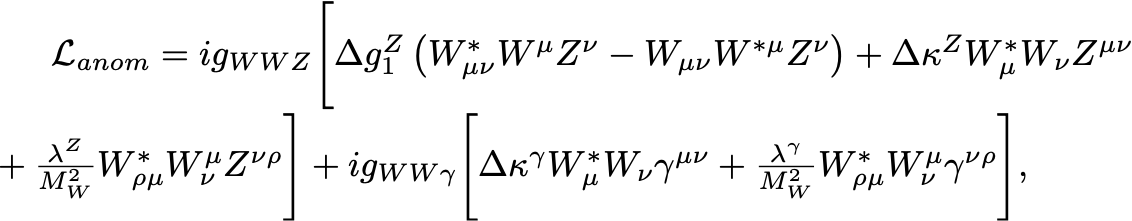
\includegraphics[width=\textwidth]{./sections/gobbets/Lagrangian.png}
%\begin{eqnarray}
%{\cal L}_{anom} & = & i g_{WWZ} \Biggl[
% \Delta g_1^Z \left( W^*_{\mu\nu}W^\mu Z^\nu - W_{\mu\nu}W^{*\mu} Z^\nu \right)
%+\Delta\kappa^Z W^*_\mu W_\nu Z^{\mu\nu} \nonumber \\
% & &+
% \frac{\lambda^Z}{M_W^2} W^*_{\rho\mu} W^\mu_\nu Z^{\nu\rho} \Biggr]
%+i g_{WW\gamma} \Biggl[ 
% \Delta\kappa^\gamma W^*_\mu W_\nu \gamma^{\mu\nu}
%+\frac{\lambda^\gamma}{M_W^2} W^*_{\rho\mu} W^\mu_\nu\gamma^{\nu\rho}
% \Biggr], \nonumber
%\end{eqnarray}

where $X_{\mu\nu} \equiv \partial_\mu X_{\nu} - \partial_\nu X_{\mu}$
and the overall coupling factors are $g_{WW\gamma}=-e$,
$g_{WWZ}=-e\cot\theta_w$.
This is the most general Lagrangian that conserves $C$ and $P$
separately and electromagnetic gauge invariance requires that there
is no equivalent of the $\Delta g_1^Z$ term for the photon coupling.

In order to avoid a violation of unitarity, these couplings are often
included only after suppression by dipole form factors,

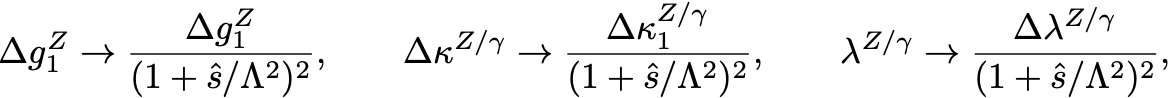
\includegraphics[width=0.9\textwidth]{./sections/gobbets/Dipole.png}

%\begin{equation}
%\Delta g_1^Z \rightarrow \frac{\Delta g_1^Z}{(1+\hat{s}/\Lambda^2)^2}, \qquad
%\Delta \kappa^{Z/\gamma} \rightarrow \frac{\Delta \kappa_1^{Z/\gamma}}{(1+\hat{s}/\Lambda^2)^2}, \qquad
%\lambda^{Z/\gamma} \rightarrow \frac{\Delta \lambda^{Z/\gamma}}{(1+\hat{s}/\Lambda^2)^2},
%\end{equation}
where $\hat{s}$ is the vector boson pair invariant mass and $\Lambda$
is an additional parameter giving the scale of new physics, which should
be in the TeV range.
These form factors should be produced by the new physics associated
with the anomalous couplings and this choice is somewhat
arbitrary. The use of the form factors can be disabled as described
below.  The file {\tt input.ini} contains the values of the $6$
parameters which specify the anomalous couplings.  If the input file
contains a negative value for the form-factor scale then the
suppression factors described above are not applied.


\bottomheading{$WW$+$ZZ$ interfering, process 8211}
This process calculable at leading LO and next-to-leading order NLO.
This process describes a specific final state which is accesible both
from the decay to two $W$'s and two $Z$'s.  The two processes can thus
interfere.

This process has been treated in several papers, \cite{Campbell:1999ah,Campbell:2011bn,Boughezal:2016wmq,Campbell:2022gdq}.

\midheading{$WH$ production, processes 91-100, 900}
\label{subsec:wh}

This process can be calculated at LO, NLO, and NNLO.
These processes represent the production of a $W$ boson which subsequently
decays leptonically, in association with a Standard Model Higgs boson that
decays into a tau pair ({\tt nproc=91, 96}),
decays into a $b$-quark pair ({\tt nproc=92, 97}),
a pair of photons ({\tt nproc=93, 98}),
or a pair of $W$-bosons ({\tt nproc=94, 99}),
a pair of $Z$ bosons ({\tt nproc=95, 100}).
Note that in the cases of Higgs decay to $W$,($Z$) pairs,
below the $W$,($Z$) pair threshold
one of the $W$,($Z$) bosons is virtual
and therefore one must set {\tt zerowidth=.false.}.
The calculation may be performed at NNLO for these processes.

Radiation from the bottom quarks in the decay, an NLO effect, is included in  ({\tt nproc=920, 970}).
\texttt{nproc=900} may be used to compute the sum over both W charges in
one run (with the decay products 3 and 4 representing lepton and antilepton
respectively). This sum is performed by adjustng the CKM matrix to allow both charges of the $W$ boson.

When {\tt removebr} is {\tt .true.}, neither the $W$ boson nor the Higgs decays.

For more information on this
process see refs.~\cite{Campbell:2016jau,Boughezal:2016wmq,Campbell:2022gdq}.
NLO calculations can be performed by subtraction, zero-jettiness
slicing and $q_T$-slicing.  NNLO calculations can be performed by
zero-jettiness slicing and $q_T$-slicing.  

\midheading{$ZH$ production, processes 101--110}
\label{subsec:zh}

These processes represent the production of a $Z$ boson (or virtual photon)
in association with a Standard Model Higgs boson that
decays into a bottom quark pair ({\tt nproc=101-103}),
or decays into a pair of photons ({\tt nproc=104-105})
or a pair of $W$ bosons ({\tt nproc=106-108}),
or a pair of $Z$ bosons ({\tt nproc=109}),
or a pair of $\tau$'s ({\tt nproc=110}).

The $Z$ subsequently decays into
either an $e^+ e^-$ pair ({\tt nproc=101, 106, 109}), neutrinos ({\tt nproc=102, 107})
or a bottom quark pair ({\tt nproc=103, 108}).
The calculation may be performed at NLO, although radiation from the
bottom quarks in the decay of the Higgs (or the $Z$, for processes
{\tt 103, 108}) is not included.
Radiation from the bottom quarks in the decay of the Higgs is included in ({\tt nproc=1010}).

When {\tt removebr} is true in processes {\tt 101, 106, 109}, neither the $Z$ boson
nor the Higgs decays.

For more information on this
process see refs.~\cite{Campbell:2016jau,Boughezal:2016wmq,Campbell:2022gdq}.
NLO calculations can be performed by subtraction, zero-jettiness
slicing and $q_T$-slicing.  NNLO calculations can be performed by
zero-jettiness slicing and $q_T$-slicing.  

\midheading{Higgs production, ($m_t=\infty$), processes 111--121}
\label{subsec:h}

This process is calculable at leading LO, 
at next-to-leading order NLO, and at next-to-next-to-leading order NNLO. 

These processes represent the production of a Standard Model Higgs
boson that decays either into a bottom quark
pair ({\tt nproc=111}), a pair of tau's ({\tt nproc=112}), 
a $W^+W^-$ 
pair that further decays leptonically ({\tt nproc=113}) 
a $W^+W^-$ pair where the $W^-$ decays hadronically ({\tt nproc=114,115}) 
or a $ZZ$ pair ({\tt nproc=116-118}) . In addition, the loop-level decays of the Higgs 
into a pair of photons ({\tt nproc=119}) and the $Z\gamma$ decay are included
({\tt nproc=120,121}).

For the case of $W^+W^-$ process {\tt nproc=115} gives the contribution 
of radiation from the hadronically decaying $W^-$.
Process {\tt 114} may be run at NLO with the option {\tt todk},
including radiation in the decay of the hadronically decaying $W^-$.~\footnote{
We have not included the case of a hadronically decaying $W^+$; it can
be obtained from processes {\tt nproc=114,115} by performing the
substitutions $\nu \to e^-$ and $e^+ \to \bar{\nu}$.}
For the case of a $ZZ$ decay,
the subsequent decays can either be into a pair of muons and a pair of electrons
({\tt nproc=116)}, a pair of muons and neutrinos ({\tt nproc=117}) or
a pair of muons and a pair of bottom quarks ({\tt nproc=118}).

At LO the relevant diagram
is the coupling of two gluons to the Higgs via a top quark loop.
This calculation is performed in the limit of infinite top quark mass, so that 
the top quark loop is replaced by an effective operator. This corresponds
to the effective Lagrangian,
\begin{equation}
\mathcal{L} = \frac{1}{12\pi v} \, G^a_{\mu\nu} G^{\mu\nu}_a H \;,
\label{eq:HeffL}
\end{equation}
where $v$ is the Higgs vacuum expectation value and $G^a_{\mu\nu}$ the
gluon field strength tensor.
The calculation may be performed at NLO, although radiation from the
bottom quarks in the decay of processes {\tt 111} and {\tt 118} is not yet included.

%At the end of the output the program will also display the cross section rescaled
%by the constant factor,
%\begin{equation}
%\frac{\sigma_{\rm LO}(gg \to H, \mbox{finite}~m_t)}{\sigma_{\rm LO}(gg \to H, m_t \to \infty)} \;.
%\label{eqn:hrescale}
%\end{equation}
%For the LO calculation this gives the exact result when retaining a finite value for $m_t$,
%but this is only an approximation at NLO. The output histograms are not rescaled in this way.

When {\tt removebr} is true in processes {\tt 111,112,113,118},
the Higgs boson does not decay.

Process {\tt 119} implements the decay of the Higgs boson into two photons
via loops of top quarks and $W$-bosons.
The decay is implemented using the formula Eq.(11.12) from ref.~\cite{Ellis:1991qj}.
When {\tt removebr} is true in process {\tt 119} the Higgs boson does not decay.

Processes {\tt 120} and {\tt 121} implement the decay of the Higgs boson into an lepton-antilepton
pair and a photon. As usual the production of a charged lepton-antilepton pair is mediated by a 
$Z/\gamma^*$ (process {\tt 120}) and the production of three types of neutrinos 
$\sum  \nu \bar{\nu}$ by a $Z$-boson (process {\tt 121}). These processes are implemented 
using a generalization of the formula of \cite{Djouadi:1996yq}. (Generalization to take into
account off-shell $Z$-boson and adjustment of the sign of $C_2$ in their Eq.(4)).

\midheading{$H \to W^+W^-$ production, ($m_t=$~finite), processes 123-127}
These processes represent the production of a Higgs boson that decays to $W^+ W^-$,
with subsequent decay into leptons. For process {\tt 123}, the exact form of the triangle
loop coupling a Higgs boson to two gluons is included, with both top and bottom quarks
circulating in the loop. This is to be contrasted with process {\tt 113} in which only the
top quark contribution is included in the effective coupling approach.

Process {\tt 124} includes only the effect of the interference of the
Higgs and $gg \to W^+W^-$ amplitudes, as described in ref.~\cite{Campbell:2011cu}.
The calculation is available at LO only. LO corresponds to $O(\alpha_s^2)$ in this case.
The calculation of loops containing the third quark generation
includes the effect of the top quark mass (but $m_b=0$), while the first two
generations are considered massless. For numerical stability, a small cut on the
transverse momentum of the $W$ bosons is applied: $p_T(W)>0.05$~GeV for loops
containing massless (first or second generation) quarks, $p_T(W)>2$~GeV for $(t,b)$
loops. This typically removes less than $0.1$\% of the cross section. The
values of these cutoffs can be changed by editing \verb|src/HWW/gg_WW_int.f| and recompiling.

Process {\tt 125} includes all $gg$-initiated diagrams that have a Higgs boson in the $s$-channel,
namely the square of the $s$-channel Higgs boson production and the interference with the diagrams
that do not contain a Higgs boson, (i.e. $gg \to W^+W^- \to \nu_e e^+ e^- \bar{\nu_e}$),
i.e.~$|M_H|^2+2 |M_H^* M_{WW}|$.

The result for the square of the box diagrams alone, i.e. the process
$gg \to W^+W^- \to \nu_e e^+ e^- \bar{\nu_e}$, may be obtained by running process
{\tt nproc=61} with {\tt part=virt} and {\tt ggonly=.true.}

Process {\tt 126} calculates the full result for this process from  $gg$-initiated diagrams.
This includes diagrams that have a Higgs boson in the $s$-channel, the continuum $W^+W^-$
diagrams described above and their interference, i.e.~$|M_{H}+M_{WW}|^2$.

Process {\tt 127} calculates the full result for this process for  $gg$-initiated box
diagrams alone, $gg \to W^+W^-$, i.e.~$|M_{WW}|^2$.

\midheading{$H \to ZZ \to e^- e^+ \mu^- \mu^+$ production, ($m_t=$~finite), processes 128-133}
These processes represent the production of a Higgs boson that decays to $Z Z$,
with subsequent decay into charged leptons. For process {\tt 128}, the exact form of the triangle
loop coupling a Higgs boson to two gluons is included, with both top and bottom quarks
circulating in the loop. This is to be contrasted with process {\tt 116} in which only the
top quark contribution is included in the effective coupling approach.

Process {\tt 129} includes only the effect of the interference of the
Higgs and $gg \to ZZ$ amplitudes.
The calculation is available at LO only. LO corresponds to $O(\alpha_s^2)$ in this case.
The calculation of loops containing the third quark generation
includes the effect of both the top quark mass and the bottom quark, while the first two
generations are considered massless. For numerical stability, a small cut on the
transverse momentum of the $Z$ bosons is applied: $p_T(Z)>0.05$~GeV.
This typically removes less than $0.1$\% of the cross section. The
values of these cutoffs can be changed by editing \verb|src/ZZ/getggZZamps.f| and recompiling.

Process {\tt 130} includes all $gg$-initiated diagrams that have a Higgs boson in the $s$-channel,
namely the square of the $s$-channel Higgs boson production and the interference with the diagrams
that do not contain a Higgs boson, (i.e. $gg \to Z/\gamma^*+Z/\gamma^* \to e^- e^+ \mu^- \mu^+$),
i.e.~$|M_H|^2+2 |M_H^* M_{ZZ}|$.

Process {\tt 131} calculates the full result for this process from  $gg$-intitiated diagrams.
This includes diagrams that have a Higgs boson in the $s$-channel, the continuum $ Z/\gamma^*+Z/\gamma^*$
diagrams described above and their interference, i.e.~$|M_H+M_{ZZ}|^2$.


Process {\tt 132}  gives the result for the square of the box diagrams alone, i.e. the process
$gg \to Z/\gamma^*+Z/\gamma^* \to e^- e^+ \mu^- \mu^+$, i.e.~$|M_{ZZ}|^2$.

Process {\tt 133} calculates the interference for the $qg$ initiated process.

For those processes that include contributions from the Higgs boson, the form
of the Higgs propagator may be changed by editing the file
{\tt src/Need/sethparams.f}.  If the logical variable {\tt CPscheme} is
changed from the default value {\tt .false.} to {\tt .true.} then the
Higgs propagator is computed using the ``bar-scheme'' that is
implemented in the HTO code of G. Passarino~\cite{Goria:2011wa,Passarino:2010qk}.
The value of the Higgs boson width has been computed with v1.1 of the
HTO code, for Higgs masses in the interval $50 < m_H< 1500$~GeV.  These
values are tabulated, in $0.5$~GeV increments, in the file
{\tt Bin/hto\_output.dat}.  The widths for other masses in this range
are obtained by linear interpolation.

% \bottomheading{Specifying other final states}
% \label{specifyingZdecays}
% As described above, these processes refer to a final state 
% $e^- e^+ \mu^- \mu^+$.  It is however possible to specify a final state
% that corresponds to a different set of $Z$ boson decays.  This is achieved
% by altering the value of {\tt NPROC} in the input file by appending a
% period, followed by two 2-character strings that identify each of the decays.
% Possible values for the strings, and the corresponding decays, are
% shown in the table below.
% \begin{center}
% \begin{tabular}{ll}
% string & $Z$ decay \\
% \hline
% {\tt el,EL} & $(e^-,e^+)$ \\
% {\tt mu,MU,ml,ML} & $(\mu^-,\mu^+)$ \\
% {\tt tl,TL} & $(\tau^-,\tau^+)$ \\
% {\tt nu,NU,nl,NL} & $(\nu,\bar\nu) \times 3$ \\
% {\tt bq,BQ} & $(b,\bar b)$ \\
% \end{tabular}
% \end{center}
% Note that, for the case of neutrino decays, the sum over three flavours of
% neutrino is performed.  The labelling of the particles in the output is best
% understood by example.  Setting {\tt nproc=132.ELNU} corresponds to the
% process $gg \to Z/\gamma^*+Z/\gamma^* \to e^-(p_3) e^+(p_4) \nu(p_5) \bar\nu(p_6)$.
% Note that the default process corresponds to the string {\tt ELMU} so that,
% for instance {\tt nproc=132.ELMU} is entirely equivalent to
% {\tt nproc=132}.
% The effect of changing the lepton flavour is only seen in the output
% of LHE events, where the correct mass is then used when producing the
% event record.


\midheading{$e^- e^+ \nu_e \bar \nu_e$ production, processes 1281, 1311, 1321}

These processes compute cross sections relevant for the final state
$e^- e^+ \nu_e \bar \nu_e$, i.e. with charged leptons and neutrinos
from the same (electron) doublet.  As a result they receive
contributions from diagrams with resonant $ZZ$ propagators and
resonant $WW$ propagators.  Process {\tt 1281} only includes
amplitudes containing a Higgs boson (c.f. processes {\tt 123} and {\tt 128}).
Process {\tt 1321} only includes continuum (box-diagram)
amplitudes (c.f. processes {\tt 127} and {\tt 132}).  Process {\tt 1311}
includes both amplitudes and the effects of the interference
between them (c.f. processes {\tt 126} and {\tt 131}).

%   The effect of
% the interference between the $WW$ and $ZZ$ diagrams can be assessed
% by, for instance, comparing process {\tt 1281} with the sum of
% processes {\tt 123} and one-third of {\tt 128.ELNU}, where the
% weighting is to divide out the natural sum over three neutrin\ o
% flavours in process {\tt 128.ELNU}.
%
% Event generation is not available for these processes at present.

\midheading{$e^- e^+ \nu \bar \nu$ production, processes 1282, 1312, 1322}

These processes compute cross sections relevant for the final state
$e^- e^+ \nu \bar \nu$, i.e. an electron pair and a sum over all three
flavours of neutrino.  For muon and tau neutrinos, only $ZZ$ diagrams
contribute.  For electron neutrinos there are contributions from
diagrams with resonant $ZZ$ propagators and resonant $WW$ propagators.
Process {\tt 1282} only includes amplitudes containing a Higgs boson
(c.f. processes {\tt 123} and {\tt 128}). Process {\tt 1322} only
includes continuum (box-diagram) amplitudes (c.f. processes {\tt 127}
and {\tt 132}).  Process {\tt 1312} includes both amplitudes and the
effects of the interference between them (c.f. processes {\tt 126} and
{\tt 131}).

% The effect of the interference between the $WW$ and $ZZ$
% diagrams can be assessed by, for instance, comparing process {\tt 1282}
% with the sum of processes {\tt 123} and {\tt 128.ELNU}.
% 
% Event generation is not available for these processes at present.

\midheading{$H+b$ production, processes 136--138}
\label{subsec:Hb}

These processes represent the production of a Standard Model Higgs
boson that decays into a pair of bottom quarks,
in association with a further bottom quark. The initial state at lowest order
is a bottom quark and a gluon.
The calculation may be performed at NLO, although radiation from the
bottom quarks in the Higgs decay is not included.
For more details on this calculation, please see Ref.~\cite{Campbell:2002zm}.

For this process, the matrix elements are divided up into a number of
different sub-processes, so the user must sum over these after performing
more runs than usual. At lowest order one can proceed as normal, using
{\tt nproc=136}. For a NLO calculation, the sequence of runs is as follows:
\begin{itemize}
\item Run {\tt nproc=136} with {\tt part=virt} and {\tt part=real} (or, both
at the same time using {\tt part=tota});
\item Run {\tt nproc=137} with {\tt part=real}.
\end{itemize}
The sum of these yields the cross-section with one identified $b$-quark in
the final state. To calculate the contribution with two $b$-quarks in the
final state, one should use {\tt nproc=138} with {\tt part=real}.

When {\tt removebr} is {\tt .true.}, the Higgs boson does not decay.

\midheading{$t\bar{t}$ production with 2 semi-leptonic decays, processes 141--145}
\label{subsec:ttbar}

These processes describe $t \bar{t}$ production including semi-leptonic
decays for both the top and the anti-top.
Since version 6.2 we have updated this to use the one-loop amplitudes of
ref.~\cite{Badger:2011yu}. The code for the virtual amplitudes now runs
about three times faster than earlier versions where the virtual
amplitudes of ref.~\cite{Korner:2002hy} were used.
Switching {\tt zerowidth} from {\tt .true.} to {\tt .false.} only affects
the $W$ bosons from the top quark decay, because our method of including spin
correlations requires the top quark to be on shell.

Process {\tt 141} includes all corrections, i.e.\ both radiative corrections
to the decay and to the production. This process is therefore the
basic process for the description of top production where both quarks
decay semi-leptonically.  When {\tt removebr} is true in process {\tt 141},
the top quarks do not decay.
When one wishes to calculate observables related to the decay of the top
quark, {\tt removebr} should be false in process {\tt 141}.
The LO calculation proceeds as normal.
At NLO, there are two options:
\begin{itemize}
\item {\tt part=virt, real} or {\tt tota} : final state radiation is included
in the production stage only
\item {\tt part = todk} : radiation is included in the decay of the top
quark also and the final result corresponds to the sum of real and virtual
diagrams.
Note that these runs automatically perform an extra integration, so
will take a little longer.
\end{itemize}

Process {\tt 142} includes only the corrections in
the semileptonic decay of the top quark. Thus it is of primary
interest for theoretical studies rather than for physics applications.
Because of the method that we have used to include the radiation in the decay,
the inclusion of the corrections in the decay does not change the
total cross section. This feature is explained in section 6 of ref.~\cite{Campbell:2012uf}.

In the case of process {\tt 145}, there are no spin correlations in
the decay of the top quarks. The calculation is performed by
multiplying the spin summed top production cross section, by the decay
matrix element for the decay of the $t$ and the $\bar{t}$. These
processes may be used as a diagnostic test for the importance of the
spin correlation.

\midheading{$t\bar{t}$ production with decay and a gluon, process 143}

This process is only calculable at leading order LO.
This process describes lowest order $t \bar{t}+g$ production
including two leptonic decays $t \to b l \nu$.
When {\tt removebr} is true, the top quarks do not decay.
This LO process only includes radiation in production.
                             
\midheading{$t\bar{t}$ production with one hadronic decay, processes 146--151}

This process is calculable at leading LO and next-to-leading order NLO.
These processes describe the hadronic production of a pair of top
quarks, with one quark decaying hadronically and one quark decaying
semi-leptonically.  For processes {\tt 146--148}, the top quark decays
semi-leptonically whereas the anti-top quark decays hadronically.  For
processes {\tt 149--151}, the top quark decays hadronically whereas the
anti-top quark decays semi-leptonically.  The base processes for
physics are process {\tt 146} and {\tt 149} which include
radiative corrections in both production and decay.  Switching {\tt zerowidth} from
{\tt .true.} to {\tt .false.} only affects the $W$ bosons from the top
quark decay, because our method of including spin correlations
requires the top quark to be on shell.
When one wishes to calculate observables related to the decay of the top
quark, {\tt removebr} should be false in processes {\tt 146} and {\tt 149}.
The LO calculation proceeds as normal. At NLO, there are two options:
\begin{itemize}
\item {\tt part=virt, real} or {\tt tota} : final state radiation is included
in the production stage only
\item {\tt part = todk} : radiation is included in the decay of the top
quark also and the final result corresponds to the sum of real and virtual
diagrams.
Note that these runs automatically perform an extra integration, so
will take a little longer.
\end{itemize}


Processes {\tt 147} and {\tt 150} include only the radiative
corrections in the decay of the top quark without including
the radiative corrections in the hadronic decay of the $W$-boson.
Because of the method that we have used to include the radiation in the decays,
the inclusion of the corrections in this stage of the decay does not change the
total cross section.
Process {\tt 148} ({\tt 151}) includes only the radiative corrections
in the hadronic decay of the $W$-boson coming from the anti-top (top).
The inclusion of the corrections in this stage of the decay increases the
partial width by the normal $\alpha_s/\pi$ factor.
                        
\midheading{$Q\overline{Q}$ production, processes 157--159}
These processes are calculable at leading LO and next-to-leading order NLO.
These processes calculate the production of heavy quarks
({\tt 157} for top, {\tt 158} for bottom and {\tt 159} for charm) up to NLO
using the matrix elements of ref.~\cite{Nason:1987xz}. No decays
are included.
                        
\midheading{$t{\bar t}+$~jet production, process 160}
This process calculates the production of top quarks and a single jet
at LO, without any decay of the top quarks.
                                
\midheading{Single-top-quark production and decay at NNLO, process 1610}
\label{single-top-quark-production-and-decay-at-nnlo}

This calculation is based on ref.~\cite{Campbell:2020fhf}. See also
ref.~\cite{Campbell:2021qgd} for the role of double-DIS scales and the
relevancy for PDFs.

This process can be run by using process number 1610. The resulting
histograms and cross-sections are printed for a strict fixed-order
expansion as well as for a naive addition of all contributions. The
fixed-order expansion assembles pieces according to the following
formula. Please see ref.~\cite{Campbell:2020fhf} for more details.

\[\begin{aligned}
\mathrm{d}\sigma_{\text{LO}} & = \frac{1}{\Gamma_t^{(0)}}
\mathrm{d}\sigma^{(0)}\otimes\mathrm{d}\Gamma_t^{(0)} \,,\\
\mathrm{d}\sigma_{\delta \text{NLO}} & = \frac{1}{\Gamma_t^{(0)}} \Bigg[ 
\mathrm{d}\sigma^{(1)}\otimes\mathrm{d}\Gamma_t^{(0)} + 
\mathrm{d}\sigma^{(0)}\otimes\left(\mathrm{d}\Gamma_t^{(1)} 
- \frac{\Gamma_t^{(1)}}{\Gamma_t^{(0)}} \mathrm{d}\Gamma_t^{(0)}  \right)
\Bigg] \,,\\
\mathrm{d}\sigma_{\delta \text{NNLO}} & = \frac{1}{\Gamma_t^{(0)}} \Bigg[
\mathrm{d}\sigma^{(2)}\otimes\mathrm{d}\Gamma_t^{(0)} + 
\mathrm{d}\sigma^{(1)}\otimes\left(
\mathrm{d}\Gamma_t^{(1)} - 
\right) \\
& \qquad\qquad  + \mathrm{d}\sigma^{(0)}\otimes \left(
\mathrm{d}\Gamma_t^{(2)} - 
\frac{\Gamma_t^{(2)}}{\Gamma_t^{(0)}}\mathrm{d}\Gamma_t^{(0)}
-\frac{\Gamma_t^{(1)}}{\Gamma_t^{(0)}} \left(
\mathrm{d}\Gamma_t^{(1)} - \frac{\Gamma_t^{(1)}}{\Gamma_t^{(0)}}
\mathrm{d}\Gamma_t^{(0)}
\right)
\right) \Bigg] \,.
\end{aligned}\]

At each order a corresponding top-decay width is used throughout all
parts. The NNLO width is obtained from ref.~\cite{Blokland:2005vq} and at
LO and NLO from ref.~\cite{Czarnecki:1990kv}. These widths agree with
numerical results obtained from our calculation of course.

This process can be run with a fixed scale or with dynamic DIS (DDIS)
scales by setting \texttt{dynamicscale\ =\ DDIS},
\texttt{renscale\ =\ 1.0} and \texttt{facscale\ =\ 1.0}.

At NNLO there are several different contributions from vertex
corrections on the light-quark line, heavy-quark line in production, and
heavy-quark line in the top-quark decay. Additionally there are one-loop
times one-loop interference contributions between all three
contributions. These contributions can be separately enabled in the
\texttt{singletop} block:

\begin{verbatim}
[singletop]
    nnlo_enable_light = .true.
    nnlo_enable_heavy_prod = .true.
    nnlo_enable_heavy_decay = .true.
    nnlo_enable_interf_lxh = .true.
    nnlo_enable_interf_lxd = .true.
    nnlo_enable_interf_hxd = .true.
    nnlo_fully_inclusive = .false.
\end{verbatim}

For a fully inclusive calculation without decay the last setting has to
be set to \texttt{.true.} and the decay and decay interference parts
have to be removed. Additionally jet requirements must be lifted, see
below.

When scale variation is enabled with DDIS scales then automatically also
a variation around the fixed scale \(\mu=m_t\) is calculated for
comparison.

This process uses a fixed diagonal CKM matrix with
\(V_{ud}=V_{cs}=V_{tb}=1\). The setting \texttt{removebr=.true.} removes
the \(W\to \nu e\) branching ratio.

This process involves complicated phase-space integrals and we have
pre-set the initial integration calls for precise differential
cross-sections with fiducial cuts. The number of calls can be tuned
overall with the multiplier setting
\texttt{integration\%globalcallmult}. For total fully inclusive
cross-sections the number of calls can be reduced by a factor of ten by
setting \texttt{integration\%globalcallmult\ =\ 0.1}, for example.

For scale variation uncertainties and PDF uncertainties we recommend to
start with the default number of calls and a larger number of warmup
iterations \texttt{integration\%iterbatchwarmup=10}, for example. For
the warmup grid no scale variation or PDF uncertainties are calculated
and this ensures a good Vegas integration grid that can be calculated
fast. The setting \texttt{integration\%callboost} modifies the number of
calls for subsequent integration iterations after the warmup. For
example setting it to \texttt{0.1} reduces the calls by a factor of ten.
This is typically enough to compute the correlated uncertainties for a
previously precisely determined central value.

At NNLO the default value for \(\tau_{\text{cut}}\) is \(10^{-3}\), which
is the value used for all the plots in our publication. We find that
cutoff effects are negligible at the sub-permille level for this choice.
We strongly recommend to not change this value.

\paragraph{Using the plotting routine with b-quark
tagging}\label{using-the-plotting-routine-with-b-quark-tagging}

The calculation has been set up with b-quark tagging capabilities that
can be accessed in both the \texttt{gencuts\_user.f90} routine and the
plotting routine \texttt{nplotter\_singletop\_new.f90}. The plotting
routine is prepared to generate all histograms shown in our publication
in ref.~\cite{Campbell:2020fhf}. By default the top-quark is
reconstructed using the leading b-quark jet and the exact W-boson
momentum, but any reconstruction algorithm can easily be implemented.

The version of the \texttt{gencuts\_user.f90} file
used for the plots in our paper~\cite{Campbell:2020fhf} is available as
\href{\mcfmprocs/Files1610/gencuts_user_singletop_nnlo.f90}{{\tt gencuts\_user\_singletop\_nnlo.f90}}.
It can be used as a guide on how to access the b-quark tagging in the \texttt{gencuts\_user} routine.

See also \texttt{nplotter\_ktopanom.f} (used for the NLO off-shell
calculation in ref.~\cite{Neumann:2019kvk} for a reconstruction of the
W-boson. It is based on requiring an on-shell W-boson and selecting the
solution for the neutrino $z$-component that gives the closest on-shell
top-quark mass by adding the leading b-quark jet.

\paragraph{Calculating fully inclusive
cross-sections}\label{calculating-fully-inclusive-cross-sections}

When calculating a fully inclusive cross-section without top-quark decay
please set \texttt{zerowidth\ =\ .true.},
\texttt{removebr\ =\ .true.} in the general section of the input file;
\texttt{inclusive\ =\ .true}, \texttt{ptjetmin\ =\ 0.0},
\texttt{etajetmax\ =\ 99.0} in the basicjets section;
\texttt{makecuts\ =\ .false.} in the cuts section; also set
\texttt{nnlo\_enable\_heavy\_decay\ =\ .false.} and
\texttt{nnlo\_enable\_interf\_lxd\ =\ .false.},
\texttt{nnlo\_enable\_interf\_hxd\ =\ .false.} and
\texttt{nnlo\_fully\_inclusive\ =\ .true.} in the singletop section.

These settings ensure that neither the decay nor any production times
decay interference contributions are included. The last setting makes
sure that only the right pieces in the fixed-order expansion of the
cross-section are included. It also ensures that the b-quark from the
top-quark decay is not jet-tagged and just integrated over.

\paragraph{Notes on runtimes and demo files}\label{notes-on-runtimes-and-demo-files}

Running the provided input file \\
\texttt{input\_singletop\_nnlo\_Tevatron\_total.ini} with
-integration\%globalcallmult=0.1 and without histograms takes about 4-5
CPU days. So depending on the number of cores, this can be run on a
single desktop within a few hours.

Running the input file \\
\texttt{input\_singletop\_nnlo\_LHC\_fiducial.ini} with the default set
of calls and histograms takes about 3 CPU months (about 3 wall-time
hours on our cluster with 45 nodes). For the fiducial cross-section
(without precise histograms) a setting of
\texttt{-integration\%globallcallmult=0.2} can also be used.

Note that \texttt{-extra\%nohistograms\ =\ .true.} has been set in these
demonstration files, so no further histograms from
\texttt{nplotter\_singletop\_new.f90} are generated.

The input file \href{\mcfmprocs/Files1610/input_singletop_nnlo_LHC_fiducial.ini}{{\tt input\_singletop\_nnlo\_LHC\_fiducial.ini}} 
together with the file \\
\href{\mcfmprocs/Files1610/gencuts_user_singletop_nnlo.f90}{{\tt gencuts\_user\_singletop\_nnlo.f90}}.
replacing \texttt{src/User/gencuts\_user.f90} reproduces the fiducial
cross-sections in ref.~\cite{Campbell:2020fhf} table 6.


                               
%\input{sections/gobbets/gobbet1650.tex}                               
\midheading{Single-top-quark production and decay at NNLO, process 1650}
\label{subsec:stop}
\label{single-top-quark-production-and-decay-at-nnlo}

This calculation is based on ref.~\cite{Campbell:2020fhf}.
This process constitutes the real correction 
needed for the complete NNLO order calculation. In other words
it is the plus-one-jet process evaluated at NLO.
                           
\midheading{Off-shell single top production in SM and SMEFT, processes 164,169}
\label{subsec:offstop}

The processes 164 and 169 represent off-shell single-top-quark and anti-top-quark production, respectively.
The calculations are performed in the complex-mass scheme.
Both the SM and contributions from the SMEFT can be calculated.
For more details on this calculation, please refer to ref.~\cite{Neumann:2019kvk}.

Dynamical double deep inelastic scattering scales can be
consistently used at NLO by setting \texttt{dynamicscale} to `DDIS'
and \texttt{scale}$=$\texttt{facscale} to 1d0. In this way the
momentum transfer along the $W$-boson $Q^2$ is used as the scale for
the light-quark-line corrections $\mu^2=Q^2$, and $\mu^2=Q^2+m_t^2$ for
the heavy-quark-line corrections. These scales are also consistently
used for the non-resonant contributions, with QCD corrections on the
$ud$-quark line, and separate QCD corrections on the bottom-quark
line.

The new block `Single top SMEFT, nproc=164,169' in the input
file governs the inclusion of SMEFT operators and corresponding
orders.  The scale of new physics $\Lambda$ can be separately set, and
has a default value of $1000$~GeV.  The flag \texttt{enable
	1/lambda4} enables the $1/\Lambda^4$ contributions, where operators
$\Qtwo, \Qfour, \Qseven$ and $\Qnine$ can contribute for the first
time.  For the non-Hermitian operators we allow complex Wilson
coefficients.  We also have a flag to disable the pure SM
contribution, leaving only contributions from SMEFT operators
either interfered with the SM amplitudes or as squared
contributions at $1/\Lambda^4$.  This can be used to directly and
quickly extract kinematical distributions and the magnitudes of
pure SMEFT contributions.

To allow for easier comparisons with previous anomalous couplings
results, and possibly estimate further higher order effects, we allow
for an anomalous couplings mode at LO by enabling the corresponding
flag.  The relations between our operators and the anomalous couplings
are

\begin{align*}
	 \delta V_L &= \Cone \frac{m_t^2}{\Lambda^2} ,\,\text{where } V_L = 1 + \delta V_L\,,\\
	 V_R &= \Ctwo{}^* \frac{m_t^2}{\Lambda^2}\,, \\
	 g_L &= -4\frac{m_W m_t}{\Lambda^2} \cdot \Cfour\,, \\
	 g_R &= -4 \frac{m_W m_t}{\Lambda^2} \cdot \Cthree{}^*\,,
\end{align*}

where $m_W$ is the $W$-boson mass, and $m_W = \frac{1}{2} g_W v$ has
been used to derive this equivalence.  Note that the minus sign for
$g_L$ and $g_R$ is different from the literature. See also the publication~~\cite{Neumann:2019kvk} for more information.

For comparisons with on-shell results one needs to add up the contributions
from processes 161 at NLO and from the virt and real contributions from 162, see above.

The analysis/plotting routine is contained in the file
`\texttt{src/User/nplotter\_ktopanom.f}', where all observables
presented in this study are implemented, and the $W$-boson/neutrino
reconstruction is implemented and can be switched on or off.

                          
\midheading{$Wt$ production, processes 180--187}
\label{subsec:wt}

These processes represent the production of a $W$ boson that decays leptonically
in association with a top quark. The lowest order diagram involves a gluon and
a bottom quark from the PDF, with the $b$-quark radiating a $W$ boson and
becoming a top quark. The calculation can be performed up to NLO.
For more details on this calculation, please see Ref.~\cite{Campbell:2005bb}.

Processes {\tt 180} and {\tt 185} produce a top quark that does not decay,
whilst in processes {\tt 181} and {\tt 186} the top quark decays leptonically.
Consistency with
the simpler processes ({\tt 180,185}) can be demonstrated by running process
{\tt 181,186} with {\tt removebr} set to true.

At next-to-leading order, the calculation includes contributions from diagrams
with two gluons in the initial state, $gg \rightarrow Wtb$. The $p_T$ of the
additional $b$ quark is vetoed according to the value of the parameter
{\tt ptmin\_bjet} which is specified in the input file. The contribution from
these diagrams when the $p_T$ of the $b$ quark is above {\tt ptmin\_bjet}
is zero. The values of this parameter and the factorization scale ({\tt facscale})
set in the input file should be chosen carefully. Appropriate values for both
(in the range $30$-$100$~GeV) are discussed in the associated paper~\cite{Campbell:2005bb}.

When one wishes to calculate observables related to the decay of the top
quark, {\tt removebr} should be false.
The LO calculation proceeds as normal. At NLO, there are two options:
\begin{itemize}
\item {\tt part=virt, real} or {\tt tota} : final state radiation is included
in the production stage only
\item {\tt part = todk} : radiation is included in the decay of the top
quark also and the final result corresponds to the sum of real and virtual
diagrams. This process can only be performed at NLO with
{\tt zerowidth = .true}. This should be set automatically.
Note that these runs automatically perform an extra integration, so
will take a little longer.
\end{itemize}

The contribution from radiation in the decay may be calculated separately using
processes {\tt 182,187}. These process numbers can be used with {\tt part=virt,real}
only. To ensure consistency, it is far simpler to use {\tt 181,186}
and this is the recommended approach.
                           
\midheading{Di-jet production, processes 190--191}
\label{subsec:dijet}

Process {\tt 190} represents di-jet production through strong interactions.
It may be calculated to LO only.

Process {\tt 191} is an ancillary process that is used in the calculation of
weak one-loop corrections to di-jet production.  
This process is calculable at leading LO and next-to-leading order NLO.
When computed at LO it gives the
contribution of weak ($O(\alpha^2)$) and mixed weak-strong ($O(\alpha\alpha_s)$)
mediated processes to di-jet production.  Please refer to Ref.~\cite{Campbell:2016dks} for details.
                          
\midheading{$H+$~jet production, $m_t=$~finite, process 200}
\label{subsec:hjetma}
This process represents the production of a Higgs boson in association
with a single jet based on
refs.~\cite{Neumann:2016dny,Neumann:2018bsx,Ellis:1987xu,Baur:1989cm,Ellis:2018hst,Budge:2020oyl}.
Decay modes are currently unsupported/untested. The top-quark mass is taken
into account exactly for the Born and real-emission parts, as well as for the singular part of the virtual corrections.
The real emission calculation is based on the one-loop, Higgs boson + 4 parton calculations
with full quark masss effects of ref.\cite{Ellis:2018hst,Budge:2020oyl}.

The finite part of the two-loop virtual corrections can be computed in
different ways by setting the input file parameter {\tt mtex}.
\begin{itemize}
    \item In a low energy asymptotic expansion in $1/m_t^k$ up to
    order $k=2,4$ by setting {\tt mtex} to $2$ or $4$ in the input
    file. This is recommended for transverse momenta up to $\simeq
    225$~GeV.

\item In a high energy expansion by setting {\tt mtex}=100 in the input
    file. This is recommended for transverse momenta beyond $450$~GeV.

\item In a rescaling approach where the finite part of the two-loop virtual
     amplitude in the effective field theory
    ($m_t=\infty$) is rescaled pointwise by the ratio of the one-loop
    amplitude computed with full $m_t$ dependence to the one-loop
    amplitude for $m_t=\infty$. This mode is the default mode and
    enabled with {\tt mtex}=0 in the input file.  This is the
    recommended approach for the intermediate energy region and for
    estimating top-mass uncertainties in the transition regions
    between these approaches.

\end{itemize}

This process is therefore calculable at leading LO and at
next-to-leading order NLO (using an approximation for the two loop
matrix element). Full NLO calculations (with the exact two-loop matrix
element) have been performed in refs.~\cite{Jones:2018hbb,Chen:2021azt,Bonciani:2022jmb}.

                                
\midheading{$H+$~jet production, processes 201--210}
\label{subsec:hjet}

These processes represent the production of a Higgs boson in association
with a single jet, with the subsequent decay of the Higgs to either
a pair of bottom quarks (processes {\tt 201,203,206})
or to a pair of tau's ({\tt 202,204,207}),
or to a pair of $W$'s which decay leptonically ({\tt 208}),
or to a pair of $Z$'s which decay leptonically ({\tt 209}),
or to a pair of photons ({\tt 210}).

\bottomheading{$m_t=$~finite, 201,202,206,207}
The Higgs boson couples to a pair of gluons via a loop of heavy fermions
which, in the Standard Model, is accounted for almost entirely by including
the effect of the top quark alone. For processes {\tt 201,202,206,207}, the
matrix elements include the full dependence on the top quark mass.
The calculation can only be performed at LO.
The LO full $m_t$ dependence calculation implements results of refs.\cite{Ellis:1987xu,Baur:1989cm}.
However, the Higgs boson can either be the Standard Model one
(processes {\tt 201,202}) or a pseudoscalar ({\tt 206,207}).
Note that the pseudoscalar case corresponds, in the heavy top limit, to the effective Lagrangian,
\begin{equation}
\mathcal{L} = \frac{1}{8\pi v} \, G^a_{\mu\nu} \widetilde G^{\mu\nu}_a A \;,
\end{equation}
where $\widetilde G^{\mu\nu}_a = i\epsilon^{\mu\nu\alpha\beta}
 G_{\alpha\beta}^a$.
The interaction differs from the scalar case in by a factor of $3/2$
and hence the rate is increased by a factor of $(3/2)^2$.


\bottomheading{$m_t=\infty$, 203,204,208,209,210}
For processes {\tt 203,204,208,209,210}, the calculation is performed in the
limit of infinite top quark mass, so that NLO and NNLO results can be obtained.
The virtual one-loop matrix elements have been implemented from
refs~\cite{Ravindran:2002dc} and~\cite{Schmidt:1997wr}.
Phenomenological results have previously been
given in refs.~\cite{deFlorian:1999zd},\cite{Ravindran:2002dc}
and \cite{Glosser:2002gm}.
Note that the effect of radiation from the bottom quarks in process {\tt 203}
is not included.
NNLO corrections have only been implemented for processes {\tt 204} and {\tt 210},
using the 1-jettiness slicing approach described in  ref.~\cite{Campbell:2019gmd}.
When {\tt removebr} is true in processes {\tt 201}, {\tt 203}, {\tt 206}, {\tt 208}, {\tt 209}
and {\tt 210}, the Higgs boson does not decay.

                           
\midheading{Higgs production via WBF, processes 211--217}
\label{subsec:wbf}

These processes provide predictions for the production of a Higgs boson in
association with two jets via weak-boson fusion (WBF). The Higgs boson
subsequently decays to either a pair of bottom quarks
(processes {\tt 211, 216}), to a pair of tau's ({\tt 212, 217}),
to a pair of $W$ bosons ({\tt 213}),
to a pair of $Z$ bosons ({\tt 214}),
or to a pair of photons ({\tt 215}).
For more details on this calculation, please see Ref.~\cite{Berger:2004pca}.

Calculations can be performed up to NLO for processes {\tt 211}--{\tt 215}.
In addition to this, processes {\tt 216} and {\tt 217} provide the lowest
order calculation of the WBF reaction which radiates an additional jet.

When {\tt removebr} is true, the Higgs boson does not decay.
                           
\midheading{$e^-e^+ \nu_{\mu} \bar\nu_{\mu} $-pair production via WBF, processes 220,2201,222,2221}
The {\it weak} processes ({\tt nproc=220,222}) occur in $O(\alpha^6)$, 
whereas the {\it strong} processes ({\tt nproc=2201,2221}) occur in $O(\alpha^4 \alpha_S^2)$.
These processes can currently only be calculated at lowest order.
\begin{eqnarray}
&220 &  f(p_1)+f(p_2) \to  Z(e^-(p_3),e^+(p_4))Z(\mu-(p_5),\mu+(p_6)))+f(p_7)+f(p_8), [WBF]  \nonumber \\
&222 &  f(p_1)+f(p_2) \to Z(e^-(p_3),e^+(p_4))Z(\nu_\mu(p_5),\bar{\nu}_\mu(p_6)))+f(p_7)+f(p_8) [WBF]  \nonumber \\
&2201 & f(p_1)+f(p_2) \to Z(e^-(p_3),e^+(p_4))Z(\mu^-(p_5),\mu^+(p_6)))+f(p_7)+f(p_8) [strong] \nonumber \\
&2221 & f(p_1)+f(p_2) \to Z(e^-(p_3),e^+(p_4))Z(\nu_\mu(p_5),\bar{\nu}_\mu(p_6)))+f(p_7)+f(p_8) [strong]  \nonumber
\end{eqnarray}

\midheading{$\tau^+\tau^-$ production, process 221}
\label{subsec:tautau}

This process provides predictions for the production of a tau lepton
pair mediated by $\gamma^*/Z$, with subsequent leptonic decays. The
calculation is available at LO only. The relevant matrix elements are
adapted from the ones in ref.~\cite{Kleiss:1988xr}.

When {\tt removebr} is true, the tau leptons do not decay.
                                
\midheading{$\nu_e  e^+ \mu^- \mu^+$-pair production via WBF, processes 223,2231}
The {\it weak} process ({\tt nproc=223})  occurs in $O(\alpha^6)$, 
whereas the {\it strong} process occurs ({\tt nproc=2231}) in $O(\alpha^4 \alpha_S^2)$.  These processes
can currently only be calculated at lowest order.
\begin{eqnarray}
& 223  & f(p_1)+f(p_2) \to W^+(\nu_e(p_3),e^+(p_4))Z(\mu^-(p_5),\mu^+(p_6)))+f(p_7)+f(p_8) [weak]  \nonumber \\
& 2231 & f(p_1)+f(p_2) \to W^+(\nu_e(p_3),e^+(p_4))Z(\mu^-(p_5),\mu^+(p_6)))+f(p_7)+f(p_8) [strong]  \nonumber
\end{eqnarray}

\midheading{$e^- \bar\nu_{e} \nu_{\mu} \mu^+$-pair production via WBF, processes 224,2241}
The {\it weak} process ({\tt nproc=224}) occurs in $O(\alpha^6)$, 
whereas the {\it strong} process ({\tt nproc=2241}) occurs in $O(\alpha^4 \alpha_S^2)$.
These processes can currently only be calculated at lowest order.
\begin{eqnarray}
&224   & f(p_1)+f(p_2) \to W^-(e^-(p_3),\bar{\nu}_e(p_6)))W^+(\nu_\mu(p_5),\mu^+(p_4))+f(p_7)+f(p_8) [WBF]    \nonumber
\\
&2241  & f(p_1)+f(p_2) \to W^-(e^-(p_3),\bar{\nu}_e(p_6)))W^+(\nu_\mu(p_5),\mu^+(p_4))+f(p_7)+f(p_8) [strong]
\nonumber
\end{eqnarray}

\midheading{$e^- \bar\nu_{e} \mu^- \mu^+$-pair production via WBF, processes 225,2251}
The {\it weak} process occurs in $O(\alpha^6)$, 
whereas the {\it strong} process occurs in $O(\alpha^4 \alpha_S^2)$.
These processes can currently only be calculated at lowest order.
\begin{eqnarray}
&225   & f(p_1)+f(p_2) \to W^-(e^-(p_3),\bar{\nu}_e(p_4))Z(\mu^-(p_5),\mu^+(p_6)))+f(p_7)+f(p_8) [weak]    \nonumber \\
&2251  &  f(p_1)+f(p_2) \to W^-(e^-(p_3),\bar{\nu}_e(p_4))Z(\mu^-(p_5),\mu^+(p_6)))+f(p_7)+f(p_8) [strong]  \nonumber
\end{eqnarray}

%\input{sections/gobbets/gobbet222.tex}                                
\midheading{$e^- e^+ \bar\nu_{e} \nu_{e}$-pair production via WBF, processes 226}
This {\it weak} process occurs at $O(\alpha^6)$, and contains contributions, from  both $WW$ and $ZZ$ production.  
This process can currently only be calculated at lowest order.
\begin{eqnarray}
&226  &  f(p_1)+f(p_2) \to e-(p_3)+e^+(p_4)+\nu_e(p_5)+\bar{\nu}_e(p_6)+f(p_7)+f(p_8) [WBF]    \nonumber
\end{eqnarray}
                                
\midheading{$\nu_{e} e^+ \nu_{\mu} \mu^+ $-pair production via WBF, processes 228,2281}
The {\it weak} process ({\tt nproc=228})  occurs in $O(\alpha^6)$,
whereas the {\it strong} process occurs ({\tt nproc=2281}) in $O(\alpha^4 \alpha_S^2)$.
These processes can currently only be calculated at lowest order.
\begin{eqnarray}
&228  &  f(p_1)+f(p_2) \to W^+(\nu_e(p_3),e^+(p_4)))W^+(\nu_\mu(p_5),\mu^+(p_6))+f(p_7)+f(p_8) [WBF] \nonumber \\
&2281 &  f(p_1)+f(p_2) \to W^+(\nu_e(p_3),e^+(p_4)))W^+(\nu_\mu(p_5),\mu^+(p_6))+f(p_7)+f(p_8) [strong]     \nonumber
\end{eqnarray}
                         
\midheading{$e^- \bar{\nu}_{e} \mu^- \bar{\nu}_{\mu} $-pair production via WBF, processes 229,2291}
The {\it weak} process ({\tt nproc=229})  occurs in $O(\alpha^6)$,
whereas the {\it strong} process occurs ({\tt nproc=2291}) in $O(\alpha^4 \alpha_S^2)$.  
These processes can currently only be calculated at lowest order.
\begin{eqnarray}
& 229 &   f(p_1)+f(p_2) \to W^-(e^-(p_3),\bar{\nu}_e(p_4)))W^+(\mu^-(p_5),\bar{\nu}_\mu(p_6))+f(p_7)+f(p_8) [WBF]
\nonumber \\
&2291 &  f(p_1)+f(p_2) \to W^-(e^-(p_3),\bar{\nu}_e(p_4)))W^-(\mu^-(p_5),\bar{\nu}_\mu(p_6))+f(p_7)+f(p_8) [strong]
\nonumber
\end{eqnarray}
                         
\midheading{$t$-channel single top with an explicit $b$-quark, processes 231--240}
\label{subsec:stopb}

These represent calculations of the $t$-channel single top~({\tt 231}) and anti-top~({\tt 231})
processes in a scheme with four flavours of quark in the proton, so that $b$-quarks are not present in the proton.
The $b$-quark is instead explicitly included in the final state.
For more details on this calculation, please see Ref.~\cite{Campbell:2009ss}.

Processes {\tt 232} and {\tt 236} represent $t$-channel single top production in association
with a further jet and may be calculated at LO only.

Processes {\tt 233} and {\tt 238} are the complete four-flavour scheme $t$-channel single top production processes.
These are therefore the processes that should be used for most physics applications.
When one wishes to calculate observables related to the decay of the top
quark, {\tt removebr} should be false in processes {\tt 233} and {\tt 236}.
The LO calculation proceeds as normal. At NLO, there are two options:
\begin{itemize}
\item {\tt part=virt, real} or {\tt tota} : final state radiation is included
in the production stage only
\item {\tt part = todk} : radiation is included in the decay of the top
quark also and the final result corresponds to the sum of real and virtual
diagrams.
Note that these runs automatically perform an extra integration, so
will take a little longer.
\end{itemize}


Processes {\tt 234} and {\tt 239} give the extra contribution due to radiation
in top decay. These processes are mainly of theoretical interest.

Processes {\tt 235} and {\tt 240} are the leading order single top processes with an
extra radiated parton. These processes do not includes jets produced in the decay process.
                           
\midheading{$W^+W^++$jets production, processes 251,252}
These processes represent the production of two $W^+$
bosons in association with two (process {\tt 251}) or three (process {\tt 252})
jets.  The lowest order at which two positively charged $W$ bosons
can be produced is with two jets.
This process is only implemented for leptonic decays of the
$W$ particles. The calculation is available at LO only.
The calculation and code are from ref.~\cite{Melia:2010bm}.
{\tt removebr} is not implemented and has no effect.

\midheading{$WZ$~+ 2 jet production, process 253-254 }
These processes represent the production of $W$ and $Z$
bosons in association with two jets.
This process is only implemented for leptonic decays of the
$W$ and $Z$ particles. The calculation is available at LO only.



\midheading{$WZ$~+ $b$~+ jet production, process 255-256 }
These processes represent the production of $W$ and $Z$
bosons in association with two jets, one of which contains a $b$-quark.
This process is only implemented for leptonic decays of the
$W$ and $Z$ particles. The calculation is available at LO only.



\midheading{$WZ$~+ 2$b$ production, process 259-260 }
These processes represent the production of $W$ and $Z$
bosons in association with two $b$-quark jets.
This process is only implemented for leptonic decays of the
$W$ and $Z$ particles. The calculation is available at LO only.



\midheading{$Z+Q$ production, processes 261--267}
\label{subsec:ZQ}

These processes represent the production of a $Z$
boson that decays into a pair of electrons,
in association with a heavy quark, $Q$.
For more details on this calculation, please see Ref.~\cite{Campbell:2003dd}.

For processes {\tt 261}, {\tt 262}, {\tt 266} and {\tt 267} the initial
state at lowest order is the heavy quark and a gluon and
the calculation may be performed at NLO.
As for $H+b$ production, the matrix elements are divided into two
sub-processes at NLO. Thus the user must sum over these after performing
more runs than usual. At lowest order one can proceed as normal, using
{\tt nproc=261} (for $Z+b$) or {\tt nproc=262} (for $Z+c$).
For a NLO calculation, the sequence of runs is as follows:
\begin{itemize}
\item Run {\tt nproc=261} (or {\tt 262}) with {\tt part=virt} and
{\tt part=real} (or, both at the same time using {\tt part=tota});
\item Run {\tt nproc=266} (or {\tt 267}) with {\tt part=real}.
\end{itemize}
The sum of these yields the cross-section with one identified heavy quark in
the final state when {\tt inclusive} is set to {\tt .false.} . To calculate the
rate for at least one heavy quark, {\tt inclusive} should be {\tt .true.}.

For processes {\tt 263} and
{\tt 264}, the calculation uses the matrix elements for the production
of a $Z$ and a heavy quark pair and demands that one of the heavy quarks
is not observed. It may either lie outside the range of $p_T$ and $\eta$
required for a jet, or both quarks may be contained in the same jet.
Due to the extra complexity (the calculation must retain the full
dependence on the heavy quark mass), this can only be computed at LO.

When {\tt removebr} is true, the $Z$ boson does not decay.
                           
\midheading{Higgs+2 jet,processes 269}

\midheading{$H + 2$~jet production, $(m_t=\infty)$, processes 270--274}

These processes represent the production of a Standard Model Higgs boson
in association with two jets. The Higgs boson
subsequently decays to either a pair of photons ({\tt nproc=270}), a bottom quark pair ({\tt nproc=271}),
a pair of tau's ({\tt nproc=272}), a pair of leptonically decaying $W$'s ({\tt nproc=273})
or a pair of leptonically decaying $Z$'s ({\tt nproc=274}).

The matrix elements are included in the infinite top mass limit
using the effective Lagrangian approach.

When {\tt removebr} is true, the Higgs boson does not decay.
                           
\midheading{$H + 3$~jet production, ($m_t=\infty$), processes 275-279}

These processes represent the production of a Standard Model Higgs boson
in association with three jets. The Higgs boson
subsequently decays to either a bottom quark pair ({\tt nproc=275}),
or a pair of tau's ({\tt nproc=276})
or a pair of $W$'s that decay leptonically into a single generation of leptons ({\tt nproc=278})
or a pair of $Z$'s that decay leptonically into a single generation of leptons ({\tt nproc=279}).
The matrix elements are included in the infinite top mass limit
using an effective Lagrangian approach. These calculations can be
performed at LO only.

When {\tt removebr} is true, the Higgs boson does not decay.
                           
\midheading{Direct $\gamma$ production, processes 280--282}
\label{subsec:dirphot}

These processes represent the production a real photon.  Since this
process includes a real photon, the cross section diverges when the
photon is very soft or in the direction of the beam.  Thus in order to
produce sensible results, the input file must supply values for both
{\tt gammptmin} and {\tt gammrapmax}. This will ensure that
the cross section is well-defined.

Currently the code computes this process up to NLO accuracy.  The
extension to NNLO~\cite{Campbell:2016lzl,Campbell:2017dqk,Campbell:2018wfu}
has not yet been made public.
                           
\midheading{Direct $\gamma$ + heavy flavour production, processes 283--284}
\label{subsec:heavyfl}

These processes represent the production a real photon with a $b$
quark or a $c$ quark Since this process includes a real photon, the
cross section diverges when the photon is very soft or in the
direction of the beam.  Thus in order to produce sensible results, the
input file must supply values for both {\tt gammptmin} and {\tt
gammrapmax}. This will ensure that the cross section is
well-defined.

The calculation of process {\tt 283}--{\tt 284} is only available at leading order.
                           
\midheading{$g(-p_1)+g(-p_2) \to  \gamma(p_3)+\gamma(p_4)$}
This process computes the contribution of light-quark loops
to the process $gg \to \gamma\gamma$.  It is calculable at leading LO
and next-to-leading order NLO.
The calculation and a phenomenological analysis are described
in Ref.~\cite{Campbell:2016yrh}.
This process includes the one-loop gluon-gluon contribution as
given in ref.~\cite{Bern:2002jx}.

\midheading{$g(-p_1)+g(-p_2) \to  \gamma(p_3)+\gamma(p_4)$, (top loops at LO)}
This process calculable at leading LO and next-to-leading order NLO.

This process computes the contribution of quark loops ($n_f = 5$ light
quarks and top quarks) to the process $gg \to \gamma\gamma$.  It is
calculable at leading LO and next-to-leading order NLO, although the
effect of top-quark loops are only included at LO.  The calculation
and a phenomenological analysis are described in
Ref.~\cite{Campbell:2016yrh}.

\midheading{Diphoton production}

\label{subsec:gamgam}
Process 285 represents the production of a pair of real photons. Since     
this process includes two real photons, the cross section diverges when    
one of the photons is very soft or in the direction of the beam. Thus in   
order to produce sensible results, the input file must supply values for  
both ptmin$_{photon}$ and etamax$_{photon}$. This will ensure that the cross   
section is well-defined.

The calculation of process 285 may be performed using either the           
Frixione algorithm or standard cone isolation. Since version 10.1 also a   
fixed cone size can be specificed as well as a simple hybrid cone          
isolation, see ref.~\cite{Neumann:2021zkb}.           

This process also includes the one-loop gluon-gluon contribution as        
given in ref.~\cite{Bern:2002jx}. The 
production of a photon via parton fragmentation is included at NLO and     
can be run separately by using the frag option in part. This option        
includes the contributions from the integrated photon dipole subtraction   
terms and the LO QCD matrix element multiplied by the fragmentation        
function.

The phase space cuts for the final state photons are defined in
{\tt{input.ini}}, for multiple photon processes such as {\tt 285 -
287} the $p_T$'s of the individual photons (hardest, second hardest
and third hardest or softer) can be controlled independently.The
remaining cuts on $R_{\gamma j}$, $\eta_{\gamma}$ etc. are applied
universally to all photons. Users wishing to alter this feature should
edit the file {\tt{photon\_cuts.f}} in the directory {\tt{src/User}}.

This process can be calculated at LO, NLO, and NNLO.
NLO calculations can be performed by subtraction, zero-jettiness slicing and $q_T$-slicing. 
NNLO calculations can be performed by  zero-jettiness slicing and $q_T$-slicing. 
Input files for these 6 possibilities are given in the  link below.

The fixed-order NNLO calculation has been implemented in ref.
\cite{Campbell:2016yrh}. Transverse
momentum resummation at the level of $\text{N}^3\text{LL}+\text{NNLO}$
has been implemented in ref. \cite{Becher:2020ugp}. By including the three-loop hard
\cite{Caola:2020dfu} and beam functions
\cite{Luo:2020epw},\cite{Ebert:2020yqt},\cite{Luo:2019szz} it has been upgraded to $\text{N}^3\text{LL}'$ in ref. \cite{Neumann:2021zkb}.



\subsection{Transverse momentum resummation}

Transverse momentum resummation can be enabled for process {\tt 285} at
highest order $\text{N}^3\text{LL}'+\text{NNLO}$ with `part=resNNLOp`.
The setting `part=resNNLO` resums to order
$\text{N}^3\text{LL}+\text{NNLO}$ ($\alpha_s^2$ accuracy in improved
perturbation theory power counting) and `part=resNLO` to order
$\text{N}^3\text{LL}+\text{NLO}$. Note that process 285 with resummation
only includes the $q\bar{q}$ channel. The $gg$ channel enters at an
increased relative level of $\alpha_s$, so has to be added with process
number 2851 at order `part=resNLO` for overall
$\text{N}^3\text{LL}'+\text{NNLO}$ precision. For an overall consistent
precision of $\text{N}^3\text{LL}+\text{NNLO}$ the $gg$ channel can be
added with `part=resLO`.

Note that at fixed-order the $gg$ channel is included at NNLO
automatically at the level of $\alpha_s^2$.

The fixed-order NNLO calculation has been implemented in ref.
\cite{Campbell:2016yrh}. Transverse
momentum resummation at the level of N$^3$LL+NNLO
has been implemented in ref. \cite{Becher:2020ugp}. By including the three-loop hard
\cite{Caola:2020dfu} and beam functions
\cite{Luo:2020epw},\cite{Ebert:2020yqt},\cite{Luo:2019szz} it has been upgraded to N$^3$LL' in ref. \cite{Neumann:2021zkb}.


\midheading{$g(-p_1)+g(-p_2) \to  \gamma(p_3)+\gamma(p_4)+f(p_5)$}
Process {\tt 2861} represents the process
$gg \to \gamma\gamma g$ mediated by a loop of light quarks.
This process is calculable at leading order LO, O($\alpha_s^3$).

The calculation is described in Ref.~\cite{Campbell:2014yka}.

\midheading{$\gamma\gamma+$jet production, process 286}

Process {\tt 286}, corresponding to the production of a pair of real photons in association with a jet, can be computed at NLO.   
Since this process includes two real photons, the cross section diverges
when one of the photons is very soft or in the direction of the beam.
Thus in order to produce sensible results, the input file must supply values for both
{\tt gammptmin} and {\tt gammrapmax}. This will ensure that
the cross section is well-defined.

The calculation of process {\tt 286} may be performed at NLO using either the
Frixione algorithm~\cite{Frixione:1998jh} or standard cone isolation.  This process also includes
the one-loop gluon-gluon contribution as given in
ref.~\cite{Bern:2002jx}.  The production of a photon via parton fragmentation is included at NLO and
can be run separately by using the {\tt frag} option in {\tt part}. This option includes the contributions from the
integrated
photon dipole subtraction terms and the LO QCD matrix element multiplied by the fragmentation function.

The phase space cuts for the final state photons are defined in {\tt{input.ini}}, for multiple photon processes such
as {\tt 285 - 287} the $p_T$'s of the individual photons (hardest, second hardest and third hardest or softer) can be
controlled independently.
The remaining cuts on $R_{\gamma j}$, $\eta_{\gamma}$ etc. are applied universally to all photons. Users wishing to
alter
this feature should edit the file {\tt{photon\_cuts.f}} in the directory {\tt{src/User}}.


The calculation is described in Ref.~\cite{Campbell:2014yka}.

\midheading{$\gamma\gamma\gamma$ production, process 287}
\label{subsec:trigam}

Process {\tt 287} represents the production of three real photons.
The cross section diverges
when one of the photons is very soft or in the direction of the beam.
Thus in order to produce sensible results, the input file must supply values for both
{\tt gammptmin} and {\tt gammrapmax}. This will ensure that
the cross section is well-defined.

The calculation of process {\tt 285} may be performed at NLO using either the
Frixione algorithm~\cite{Frixione:1998jh} or standard cone isolation.  The production of a photon via parton
fragmentation is included at NLO and
can be run separately by using the {\tt frag} option in {\tt part}. This option includes the contributions from the
integrated
photon dipole subtraction terms and the LO QCD matrix element multiplied by the fragmentation function.
The phase space cuts for the final state photons are defined in {\tt{input.ini}}, for multiple photon processes such
as {\tt 285 - 287} the $p_T$'s of the individual photons (hardest, next-to hardest and softest) can be controlled
independently.
The remaining cut on $R_{\gamma j}$, $\eta_{\gamma}$ etc. are applied universally to all photons. Users wishing to alter
this feature should edit the file {\tt{photon\_cuts.f}} in the directory {\tt{src/User}}.
                                
\midheading{$\gamma\gamma\gamma\gamma$ production, process 289}
\label{subsec:fourgam}

Process {\tt 289} represents the production of four real photons.
The cross section diverges
when one of the photons is very soft or in the direction of the beam.
Thus in order to produce sensible results, the input file must supply values for both
{\tt gammptmin} and {\tt gammrapmax}. This will ensure that
the cross section is well-defined.

The calculation of process {\tt 289} may be performed at NLO using either the
Frixione algorithm~\cite{Frixione:1998jh} or standard cone isolation.  The production of a photon via parton
fragmentation is included at NLO and
can be run separately by using the {\tt frag} option in {\tt part}. This option includes the contributions from the
integrated
photon dipole subtraction terms and the LO QCD matrix element multiplied by the fragmentation function.
The phase space cuts for the final state photons are defined in {\tt{input.ini}}, for multiple photon processes such
as {\tt 285 - 289} the $p_T$'s of the individual photons (hardest, next-to hardest and softest) can be controlled
independently.
The remaining cut on $R_{\gamma j}$, $\eta_{\gamma}$ etc. are applied universally to all photons. Users wishing to alter
this feature should edit the file {\tt{photon\_cuts.f}} in the directory {\tt{src/User}}.

Note that for this process the second softest and softest photons are forced to have equal minimum $p_T$, defined
by the {\tt{[gammptmin(3rd)]}} variable in the input file.
                                
\midheading{$W\gamma$ production, processes 290-299, 2941, 2991}
\label{subsec:wgamma}

These processes represent the production of a $W$ boson which subsequently
decays leptonically, in association with a real photon.
Since this process includes a real photon, the cross section diverges
when the photon is very soft or in the direction of the beam.
Thus in order to produce sensible results, the input file must supply values for both
{\tt gammptmin} and {\tt gammrapmax}. Moreover, when the parameters {\tt zerowidth}
and {\tt removebr} are set to {\tt .false.} the decay $W \to \ell \nu$ will include
photon radiation from the lepton, so that a non-zero $R(\gamma,\ell)_{min}$
({\tt Rgalmin}) should
also be supplied. This will ensure that the cross section is well-defined.
Virtual amplitudes are taken from ref.~\cite{Dixon:1998py}.

The calculation of processes {\tt 290} and {\tt 295} may be performed
at NLO and NNLO using the Frixione algorithm~\cite{Frixione:1998jh} or standard isolation. 
The phenomenology of these processes at NNLO has been treated in ref.~\cite{Campbell:2021mlr}.
The one-loop virtual diagrams are taken from \cite{Dixon:1998py} and the two-loop virtual diagrams
are taken from \cite{Gehrmann:2011ab}.
For processes {\tt 290} and {\tt 295} the role of {\tt mtrans34cut} changes to become a cut 
on the transverse mass on the $M_{345}$ system, i.e. the photon is included with the leptons in the cut. 

Processes {\tt 292} and {\tt 297} represent the $W\gamma$+jet production
processes.  They may be computed to NLO. 

Processes {\tt 294} and {\tt 299} represent the photon-induced reactions,
$p + \gamma \to e \nu \gamma j$ and should be computed at NLO. 
Processes {\tt 2941} and {\tt 2991} represent the photon-induced reactions,
$p + \gamma \to e \nu \gamma j j$ and should be computed at NLO. 

\bottomheading{Anomalous $WW\gamma$ couplings}
Processes {\tt 290}-{\tt 297} may also be computed including the effect of anomalous $WW\gamma$ couplings, making
use of the amplitudes calculated in Ref.~\cite{DeFlorian:2000sg}. Including only dimension 6 operators
or less and demanding gauge, $C$ and $CP$ invariance gives the general form of the anomalous 
vertex~\cite{DeFlorian:2000sg},
\begin{eqnarray}
 \Gamma^{\alpha \beta \mu}_{W W \gamma}(q, \bar q, p) &=& 
  {\bar q}^\alpha g^{\beta \mu} 
    \biggl( 2 + \Delta\kappa^\gamma + \lambda^\gamma {q^2\over M_W^2} \biggr) 
 - q^\beta g^{\alpha \mu}
    \biggl( 2 + \Delta\kappa^\gamma + \lambda^\gamma {{\bar q}^2\over M_W^2}
\biggr) \nonumber \\  
&& \hskip 1 cm
 + \bigl( {\bar q}^\mu - q^\mu \bigr) 
 \Biggl[ - g^{\alpha \beta} \biggl( 
   1 + {1\over2} p^2 \frac{\lambda^\gamma}{M_W^2} \biggr) 
 +\frac{\lambda^\gamma}{M_W^2} p^\alpha p^\beta \Biggr] \,,
\end{eqnarray}
where the overall coupling has been chosen to be $-|e|$. The parameters that
specify the anomalous couplings, $\Delta\kappa^\gamma$ and $\lambda^\gamma$, are
specified in the input file as already discussed in Section~\ref{subsec:diboson}.
If the input file contains a negative value for the form-factor scale $\Lambda$
then no suppression factors are applied to the anomalous couplings.
Otherwise, the couplings are included
in MCFM only after suppression by dipole form factors,
\begin{equation}
\Delta \kappa^{\gamma} \rightarrow
 \frac{\Delta \kappa_1^{\gamma}}{(1+\hat{s}/\Lambda^2)^2}, \qquad
\lambda^{\gamma} \rightarrow
 \frac{\Delta \lambda^{\gamma}}{(1+\hat{s}/\Lambda^2)^2} \;,
\end{equation}
where $\hat{s}$ is the $W\gamma$ pair invariant mass.

The Standard Model cross section is obtained by setting $\Delta\kappa^\gamma = \lambda^\gamma = 0$.

             
\midheading{$Z\gamma$, production, processes 300, 305}
\label{subsec:zgamma}


Processes {\tt 300} and {\tt 305} represent the production of a $Z$ boson (or virtual photon for process {\tt 300})
in association with a real photon based on ref.~\cite{Campbell:2017aul}. The $Z/\gamma^*$ subsequently decays into
either an $e^+ e^-$ pair ({\tt nproc=300}) or neutrinos ({\tt nproc=305}).
Since these processes include a real photon, the cross section diverges
when the photon is very soft or in the direction of the beam.
Thus in order to produce sensible results, the input file must supply values for both
{\tt gammptmin} and {\tt gammrapmax}. Moreover, when the parameters {\tt zerowidth}
and {\tt removebr} are set to {\tt .false.} the decay $Z \to e^- e^+$ ({\tt nproc=300})
will include photon radiation from both leptons, so that a non-zero $R(\gamma,\ell)_{min}$
({\tt Rgalmin})
should also be supplied. This will ensure that the cross section is well-defined.
The calculation of processes {\tt 300} may be performed
at NNLO using the Frixione algorithm~\cite{Frixione:1998jh} or standard isolation.
The one-loop virtual diagrams are taken from \cite{Dixon:1998py} and the two-loop virtual diagrams
are taken from \cite{Gehrmann:2011ab}.

%Processes {\tt 302} and {\tt 307}  represents the production of a $Z$ boson (or virtual photon)
%in association with a real photon and an additional jet. These processes are also available at NLO including
%the full fragmentation processes. Anomalous couplings are not available for these processes.
%Processes {\tt 304} and {\tt 309}  represents the production of a $Z$ boson (or virtual photon)
%in association with a real photon and and two additional jets. These processes are available at leading order only.
%When {\tt removebr} is true in process {\tt 300} or {\tt 302} the $Z$ boson does not decay.

For the process {\tt 300}  the role of {\tt mtrans34cut} changes to become a cut
on the invariant mass on the $M_{345}$ system, i.e. the photon is included with the leptons in the cut.

\bottomheading{Anomalous $ZZ\gamma$ and $Z\gamma\gamma$ couplings}
Processes {\tt 300}-{\tt 305} may also be computed including the effect of anomalous couplings between $Z$ bosons and 
photons.
Note that, at present, the effect of anomalous couplings is not included in the gluon-gluon
initiated contributions.

The anomalous $Z\gamma Z$ vertex (not present at all in the Standard Model),
considering operators up to dimension 8, is given by~\cite{DeFlorian:2000sg},

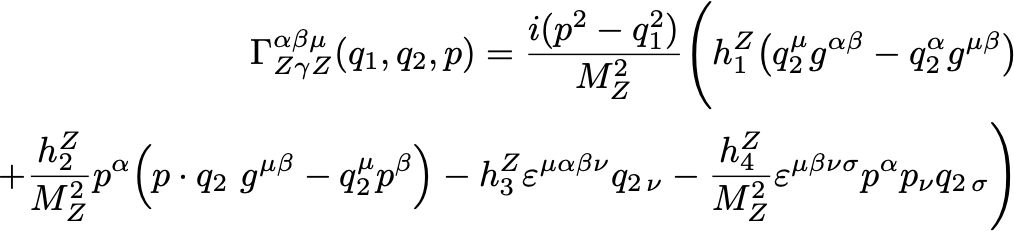
\includegraphics[width=0.9\textwidth]{./sections/gobbets/ZZgamma.png}
%\begin{eqnarray}
% && \Gamma^{\alpha \beta \mu}_{Z \gamma Z}(q_1, q_2, p) = 
%   \frac{i(p^2-q_1^2)}{M_Z^2} \Biggl( 
%   h_1^Z \bigl( q_2^\mu g^{\alpha\beta} - q_2^\alpha g^{\mu \beta}
%   \bigr) \nonumber \\
%&& + \frac{h_2^Z}{M_Z^2} p^\alpha \Bigl( p\cdot q_2\ g^{\mu\beta} -
%            q_2^\mu p^\beta \Bigr)
%   - h_3^Z \varepsilon^{\mu\alpha\beta\nu} q_{2\, \nu} 
%   - \frac{h_4^Z}{M_Z^2} \varepsilon^{\mu\beta\nu\sigma} p^\alpha
%p_\nu q_{2\, \sigma} \Biggl)
%\end{eqnarray}

where the overall coupling has been chosen to be $|e|$ (and
$\epsilon^{0123}=+1$). The non-standard $Z_\alpha(q_1) \gamma_\beta(q_2)
\gamma_\mu(p)$ momentum-space vertex can be obtained from
this equation by setting $q_1^2 \to 0$ and replacing $h_i^Z \to
h_i^\gamma$. 
The parameters that
specify the anomalous couplings, $h_i^Z$ and $h_i^\gamma$ (for $i=1\ldots 4$), are
specified in the input file as, e.g. {\tt h1(Z)} and {\tt h1(gamma)}.
If the input file contains a negative value for the form-factor scale $\Lambda$
then no suppression factors are applied to these anomalous couplings.
Otherwise, the couplings are included
in MCFM only after suppression by dipole form factors,
\begin{equation}
h_{1,3}^{Z/\gamma} \rightarrow
 \frac{h_{1,3}^{Z/\gamma}}{(1+\hat{s}/\Lambda^2)^3}, \qquad
h_{2,4}^{Z/\gamma} \rightarrow
 \frac{h_{2,4}^{Z/\gamma}}{(1+\hat{s}/\Lambda^2)^4}, \qquad
\end{equation}
where $\hat{s}$ is the $Z\gamma$ pair invariant mass. Note that these form factors are slightly
different from those discussed in Sections~\ref{subsec:diboson} and~\ref{subsec:wgamma}. The
form factors can be modified in {\ttfamily src/Need/set\_anomcoup.f}.

The Standard Model cross section is obtained by setting $h_i^Z = h_i^\gamma = 0$ for $i=1\ldots 4$.
                          
\midheading{$Z\gamma\gamma$ production processes, 301, 306}

Processes {\tt{301}} and {\tt{306}} represent the production of a $Z$ boson
(or virtual photon for process {\tt 301}) in association with two photons.   The $Z/\gamma^*$ subsequently decays into
either an $e^+ e^-$ pair ({\tt nproc=301}) or neutrinos ({\tt nproc=306}).
Since these processes include real photons, the cross section diverges
when either of the photons is very soft or in the direction of the beam.
Thus in order to produce sensible results, the input file must supply values for both
{\tt gammptmin} and {\tt gammrapmax}. Moreover, when the parameters {\tt zerowidth}
and {\tt removebr} are set to {\tt .false.} the decay $Z \to e^- e^+$ ({\tt nproc=301})
will include photon radiation from both leptons, so that a non-zero $R(\gamma,\ell)_{min}$
({\tt Rgalmin})
should also be supplied. This will ensure that the cross section is well-defined.
Anomalous couplings are not currently implemented for these processes.
                          
\midheading{$Z\gamma j$, production, processes 302, 307}
\label{subsec:zgammajet}
Processes {\tt 302} and {\tt 307} represent the production of a $Z$ boson (or virtual photon)
in association with a real photon and at least one jet.
The $Z/\gamma^*$ subsequently decays into
either an $e^+ e^-$ pair ({\tt nproc=302}) or neutrinos ({\tt nproc=307}).
Since these processes include a real photon and a jet, the cross section diverges
when the photon or jet is very soft or in the direction of the beam.
Thus in order to produce sensible results, the input file must supply values for both
{\tt gammptmin} and {\tt gammrapmax}, and {\tt ptjetmin} and {\tt etajetmax}.
 Moreover, when the parameters {\tt zerowidth}
and {\tt removebr} are set to {\tt .false.}, the decay $Z \to e^- e^+$ ({\tt nproc=302})
will include photon radiation from both leptons, so that a non-zero $R(\gamma,\ell)_{min}$
({\tt Rgalmin})
should also be supplied. This will ensure that the cross section is well-defined.
The calculation of processes {\tt 302} and {\tt 307} may be performed
at NLO using the Frixione algorithm~\cite{Frixione:1998jh} or standard isolation.
Anomalous couplings are not currently implemented for these processes.
                          
\midheading{$Z\gamma\gamma j$ and $Z\gamma j j $, 303, 304, 308 and 309}

These processes are available at LO only. The $Z/\gamma^*$ subsequently decays into
either an $e^+ e^-$ pair ({\tt nproc=303,304}) or neutrinos ({\tt nproc=308,309}).
Since these processes include a real photon and a jet, the cross section diverges
when a photon or a jet is very soft or in the direction of the beam.
Thus in order to produce sensible results, the input file must supply values for both
{\tt gammptmin} and {\tt gammrapmax}, and {\tt ptjetmin} and {\tt etajetmax}.
 Moreover, when the parameters {\tt zerowidth}
and {\tt removebr} are set to {\tt .false.} the decay $Z \to e^- e^+$ ({\tt nproc=303, 304})
will include photon radiation from both leptons, so that a non-zero $R(\gamma,\ell)_{min}$
({\tt Rgalmin})
should also be supplied. This will ensure that the cross section is well-defined.
Anomalous couplings are not currently implemented for these processes.

%Processes {\tt 303} and {\tt 308}  represents the production of a $Z$ boson (or virtual photon)
%in association with a two photons and and an additional jet. These processes are available at leading order only.
%These processes do not currently have anomalous couplings implemented.
              
\midheading{$W+Q+$~jet production processes 311--326}
\label{subsec:wQj}

These processes represent the production of a $W$
boson that decays leptonically,
in association with a heavy quark, $Q$ and an additional light jet. In
processes {\tt 311} and {\tt 316}, $Q$ is a bottom quark, whilst
processes {\tt 321} and {\tt 326} involve a charm quark.
In these processes the quark $Q$ occurs as parton PDF in the initial state.
The initial state in these processes consists of a light quark and a heavy
quark, with the light quark radiating the $W$ boson. These calculations may
be performed at LO only.

When {\tt removebr} is true, the $W$ boson does not decay.
                           
\midheading{$W+c+$~jet production, processes 331, 336}
\label{subsec:wcj}

These processes represent the production of a $W$
boson that decays leptonically,
in association with a charm quark and an additional light jet.

In contrast to processes {\tt 321} and {\tt 326} described above, the initial
state in this case consists of two light quarks, one of which is a
strange quark which radiates the $W$ boson. The calculation may
be performed at LO only.

When {\tt removebr} is true, the $W$ boson does not decay.
                           
\midheading{$Z+Q+$jet production, processes 341--357}
\label{subsec:ZQj}

These processes represent the production of a $Z$
boson that decays into a pair of electrons,
in association with a heavy quark, $Q$ and an untagged jet.
For more details on this calculation, please see Ref.~\cite{Campbell:2005zv}.

For processes {\tt 341} and {\tt 351} the initial state at lowest
order is the heavy quark and a gluon and the calculation may be
performed at NLO.  Thus in these processes the quark $Q$ occurs as
parton PDF in the initial state.  As for $H+b$ and $Z+Q$ production,
the matrix elements are divided into two sub-processes at NLO. Thus
the user must sum over these after performing more runs than usual. At
lowest order one can proceed as normal, using {\tt nproc=341} (for
$Zbj$) or {\tt nproc=351} (for $Zcj$).  For a NLO calculation, the
sequence of runs is as follows:
\begin{itemize}
\item Run {\tt nproc=341} (or {\tt 351}) with {\tt part=virt} and
{\tt part=real} (or, both at the same time using {\tt part=tota});
\item Run {\tt nproc=342} (or {\tt 352}) with {\tt part=real}.
\end{itemize}
The sum of these yields the cross-section with one identified heavy
quark and one untagged jet in the final state when {\tt inclusive} is
set to {\tt .false.} . To calculate the rate for at least one heavy
quark and one jet (the remaining jet may be a heavy quark, or
untagged), {\tt inclusive} should be {\tt .true.}.

Processes {\tt 346,347} and {\tt 356,357} are the lowest order processes that enter
the above calculation in the real contribution. They can be computed only at LO.

When {\tt removebr} is true, the $Z$ boson does not decay.
                           
\midheading{$c \overline s \to W^+$, processes 361--363}
\label{subsec:csbar}
These processes represent the production of a $W^+$ from a charm and anti-strange
quark at LO. The $W^+$ boson decays into a neutrino and a positron.

The NLO corrections to this LO process include a contribution of the form,
$g\overline s \to W^+ \overline c$. For process {\tt 361} this contribution is
calculated in the approximation $m_c=0$ at NLO. In order to perform the NLO calculation
for a non-zero value of $m_c$, one must instead sum the results of processes {\tt 362}
and {\tt 363} for {\tt part=tota}.

\midheading{$W\gamma\gamma$ production, processes 370-371}
\label{subsec:wgamgam}

These processes represent the production of a $W$ boson which subsequently
decays leptonically, in association with two real photons.
Since this process includes real photons, the cross section diverges
when the photon is very soft or in the direction of the beam.
Thus in order to produce sensible results, the input file must supply values for both
{\tt gammptmin} and {\tt gammrapmax}. Moreover, when the parameters {\tt zerowidth}
and {\tt removebr} are set to {\tt .false.} the decay $W \to \ell \nu$ will include
photon radiation from the lepton, so that a non-zero {\tt R(photon,lept)\_min} should
also be supplied. This will ensure that the cross section is well-defined.

These processes may be computed at leading order only.

\midheading{$W+Q$ production in the 4FNS, processes 401--408}
\label{subsec:wbbfilter}
These processes represent the production of a $W$ boson and one or more jets,
at least one of which is a $b$-quark, calculated in the 4-flavour number scheme (4FNS).
This implies that contributions that explicitly contain a $b$-quark in the initial state
are not included.
These processes all use the same matrix
elements as processes 20 and 25 (see section~\ref{subsec:wbb}), but make different
cuts on the final state. The final state is specified by the process number and
the value of the flag {\tt inclusive}, as shown in Table~\ref{table:wbbfilter}.
An additional flag is hard-coded into the file {\tt src/Cuts/filterWbbmas.f} to control
the inclusion of the 3-jet configuration, $(b,\overline b,j)$ when {\tt inclusive} is set to {\tt .true.}.
By default, the statement {\tt veto3jets = .false.} is included in this file. If this flag is set to {\tt .true.}
then the $(b,\overline b,j)$ contribution
is not included in processes 401, 402, 406, 407.

\begin{table}
\begin{center}
\begin{tabular}{|c|c|c|} \hline
 Process ($W^+$/$W^-$) & {\tt inclusive=.false.} & {\tt inclusive=.true.} \\
\hline
{\tt 401}/{\tt 406} & $(b)$ or $(\overline b)$ & + ($b,\overline b$) or ($b,j$) or ($\overline b,j$) \\
{\tt 402}/{\tt 407} & $(B)$ & + ($B,j$) \\
{\tt 403}/{\tt 408} & $(b,\overline b)$ & \mbox{(no extra configurations)} \\
\hline
\end{tabular}
\caption{The different final states allowed in the calculation of processes 401--408. A jet containing
both $b$ and $\overline b$ quarks is denoted by $B$ and a light (quark or gluon) jet by $j$. The inclusive
(right-hand) column also allows the final states in the exclusive (middle) column.}
\label{table:wbbfilter}
\end{center}
\end{table}

As usual, jets may be unobserved as a result of them falling outside the $p_T$
and rapidity ranges specified in the input file. In addition, the number of jets
may be different from the number of partons in the matrix element calculation as
a result of merging in the jet algorithm.

\midheading{$W+Q$ production in the 5FNS, processes 411, 416}
\label{subsec:wb5FNS}

These processes represent production of a $W$ boson in association with a
$b$-jet, computed in the 5-flavour number scheme, i.e. a $b$-quark is present in
the initial state. The lowest order processes are the same as in processes {\tt 311}, {\tt 316}.
The results at NLO are not physical cross sections since part of the corrections
are not included in order to avoid double-counting with the 4FNS process (processes
{\tt 401} and {\tt 406}). To obtain combined 4FNS+5FNS predictions, the user
should select process {\tt 421} ($W^+$) or {\tt 426} ($W^-$).
                          
\midheading{$W+Q$ production in combined 4FNS/5FNS, processes 421, 426}
\label{subsec:wbcombined}
These processes represent the production of a $W$ boson and one or more jets,
at least one of which is a $b$-quark, calculated by combining the 4- and 5-flavour results
of processes {\tt 401}, {\tt 411} (for {\tt 421}) and {\tt 406}, {\tt 416} (for {\tt 426}).
The selection of the final state is the same as for processes {\tt 401} and {\tt 406}, as
described in Section~\ref{subsec:wbbfilter}. The procedure for combining the two
calculations is described in refs.~\cite{Campbell:2008hh,Caola:2011pz}.
                          
\midheading{$W+b{\bar b}+$~jet production, processes 431,436}
\label{subsec:wbbjetmassive}

These processes represent the production of a $W$ boson which subsequently
decays leptonically, in association with a $b{\bar b}$ pair and an
additional jet. The effect of the bottom quark mass is included (in contrast to
the massless approximation used in processes {\tt 24}, {\tt 29})
and the calculation may be performed at LO only.

When {\tt removebr} is true, the $W$ boson does not decay.
                          
\midheading{Diboson+jet production, processes 461--487}
\label{subsec:dibosonjet}

These processes represent the production of a vector boson pair in association
with a jet.  They are the counterparts of the corresponding diboson process
(\texttt{nproc-400}) described above, but also including a jet in the final
state.  They may be computed to NLO.
Amplitudes are taken from refs.~\cite{Campbell:2015hya,Campbell:2016uvh,Campbell:2022qpq}.
                           
\midheading{$W+t{\bar t}$ processes 500--516}
\label{subsec:wttdecay}

These processes represent the production of a $W^\pm$ boson which subsequently
decays leptonically, in association with a $t{\bar t}$ pair. In all except processes
{\tt 500} and {\tt 510} the decays of the top and anti-top quark are included.
Processes {\tt 501,502} and {\tt 511,512} refer to the semileptonic decay of the top and antitop quarks,
with the latter process in each pair giving the radiation in the decay of the top and antitop.
Process {\tt 503} ({\tt 513}) refers to the semileptonic decay of the top (antitop)
and the hadronic decay of the antitop (top). Processes {\tt 506}({\tt 516}) gives the semileptonic
decay of the antitop(top) and the hadronic decay of the top(antitop).  Processes {\tt 506}({\tt 516})
do not give same sign lepton events, so they may be of less phenomenological importance. For this reason
we have not yet included radiation in the decay for these processes.

For processes {\tt 503}, {\tt 506}, {\tt 513}
and {\tt 516} the default behaviour is that the hadronic decay products
are clustered into jets using the supplied jet
algorithm parameters, but no cut is applied on the number of jets.
This behaviour can be altered by changing the value of the
variable {\tt notag} in the file {\tt src/User/setnotag.f}.

The top quarks are always
produced on-shell, which is a necessity for a gauge invariant result
from this limited set of diagrams, but all spin correlations are included.
Switching {\tt zerowidth} from {\tt .true.} to {\tt .false.} only affects
the $W$ bosons (both the directly produced one and from the top quark decay).
Processes {\tt 501} and {\tt 511} may be run at NLO with the option {\tt todk},
including radiation in the decay of the top quark, see section \ref{subsec:ttbar}.
                          
\midheading{$Zt{\bar t}$ production, processes 529-533}
\label{subsec:ztt}

These processes represent the production of a $Z$ boson in association
with a pair of top quarks. These processes are only available at LO.
For process {\tt 529}, neither the top quarks nor the $Z$-boson
decays.
In processes {\tt 530-533}, the top quarks are always
produced on-shell, which is a necessity for a gauge invariant result
from this limited set of diagrams.
Switching {\tt zerowidth} from {\tt .true.} to {\tt .false.} only affects
the $Z$ and the $W$ bosons from the top quark decay.
In process {\tt 530} the $Z$ boson decays into an electron pair, whilst
in {\tt 531} the decay is into a massless bottom quark pair.
In process {\tt 532--533} the $Z$ boson decays into an electron pair, whilst
one or other of the top quark or top anti-quark decays hadronically.

For processes {\tt 532} and {\tt 533} the default behaviour is that the hadronic decay products
are clustered into jets using the supplied jet
algorithm parameters, but no cut is applied on the number of jets.
This behaviour can be altered by changing the value of the
variable {\tt notag} in the file {\tt src/User/setnotag.f}.

When {\tt removebr} is true in process {\tt 530}, the top quarks and the $Z$ boson do not decay.
                          
\midheading{$Ht$ and $H\bar{t}$ production, processes 540--557}

\label{subsec:Ht}
These processes describe the production of a single top quark ({\tt 540}, {\tt 544}, {\tt 550},
{\tt 554}) or antiquark ({\tt 541}, {\tt 547}, {\tt 551}, {\tt 557}) by $W$ exchange in the
$t$-channel, in association with a Higgs boson. These processes can be performed at NLO.
For processes {\tt 540}, {\tt 541}, {\tt 550},
{\tt 551}, the top quark does not decay, but the
Higgs boson decays to $b\bar{b}$, ({\tt 540}, {\tt 541}), or to $\gamma \gamma$, ({\tt 550}, {\tt 551}).
Processes {\tt 544}, {\tt 547} and {\tt 554}, {\tt 557} include the decay of the top quark and antiquark
in the approximation in which the top quark is taken to be on shell allowing a clean separation
between production and decay.
For more details on this calculation, please see Ref.~\cite{Campbell:2013yla}.

It is possible to study the effects of anomalous couplings of the Higgs boson to the top quark and $W$ bosons. These
are parametrized by $c_{t\bar{t}H} = g_{t\bar{t}H}/g_{t\bar{t}H}^{SM}$ and $c_{WWH} = g_{WWH}/g_{WWH}^{SM}$
respectively, so that $c_{t\bar{t}H}=c_{WWH}=1$ in the SM. Different couplings may be chosen by modifying the variables
{\tt cttH} and {\tt cWWH} in the \verb|anom_higgs| section of the input file.
                          
\midheading{$Zt$ and $Z\bar{t}$ production, processes 560--569}\

\label{subsec:Zt}
These processes describe the production of a single top quark (or antiquark) by $W$ exchange in the
$t$-channel, in association with a $Z$ boson. Processes {\tt 560}, {\tt 561},
{\tt 564}, {\tt 567} can be performed at NLO.
Processes {\tt  560}-{\tt 563} are for stable top quarks, whereas processes {\tt 564}-{\tt 569}
include the decay of the top quark and antiquark
in the approximation inwhich the top quark is taken to
be on shell allowing a clean separation
between production and decay.
For more details on this calculation, please see Ref.~\cite{Campbell:2013yla}.

For processes {\tt 564} and {\tt 567} the default behaviour is that the hadronic decay products
are clustered into jets using the supplied jet
algorithm parameters, but no cut is applied on the number of jets.
This behaviour can be altered by changing the value of the
variable {\tt notag} in the file {\tt src/User/setnotag.f}.
                          
\midheading{$HH$ production, processes 601--602}
These processes represent the production of a pair of Higgs bosons.
The production proceeds through gluon-fusion one-loop diagrams involving loops
of top quarks. The formulae implemented in the code are taken from ref.~\cite{Glover:1987nx},
where the two Higgs bosons are treated as being on-shell. To enforce this
condition, the code sets zerowidth to true, overriding the value set in the input file.
The calculation can be performed at LO only, (i.e.\ one-loop order only).
Two decays of the Higgs bosons are currently foreseen, although other decays can easily be implemented.
In process {\tt 601}, one Higgs boson decays to
a pair of $b$-quarks, and the other decays to a pair of $\tau$'s.
In process {\tt 602}, one Higgs boson decays to
a pair of $b$-quarks, and the other decays to a pair of photons.

\midheading{$WH$ production, process 609}
This process represents the production of $W$ and $H$ bosons in
association with a jet, with the subsequent decay $H \to \tau^+ \tau^-$.
Both charges of the $W$ boson are summed over and, as a result, the
decay products of the $W$ boson, particles 3 and 4,
represent lepton and antilepton respectively (i.e. they do not correspond
to a neutrino and charged lepton).
It is primarily of interest as a component
part of the NNLO contributions to $WH$ production.
For further information see ref.~\cite{Campbell:2016jau}.
This process is calculable at leading LO and next-to-leading order NLO.
     
\midheading{Associated production of $WH$ and a jet, processes 610-618}
These processes represent the production of $W^\pm$ and $H$ bosons in
association with a jet, with various decays of the Higgs boson provided.
They are primarily of interest as a component
part of the NNLO contributions to $WH$ production.
For further information see ref.~\cite{Campbell:2016jau}.
This process is calculable at leading LO and next-to-leading order NLO.

\midheading{Associated production of $ZH$ and a jet, processes 620-623}
These processes represent the production of $Z$ and $H$ bosons in
association with a jet, with various decays of the Higgs boson provided.
They are primarily of interest as a component
part of the NNLO contributions to $ZH$ production.
For further information see ref.~\cite{Campbell:2016jau}.
This process is calculable at leading LO and next-to-leading order NLO.

\midheading{$Ht{\bar t}$ production, processes 640--667}
\label{subsec:htt}

These processes represent the production of a Higgs boson in association
with a pair of top quarks. The calculation can be performed at LO only.

For process {\tt 640}, neither the top quarks nor the Higgs boson
decays.
In processes {\tt 641-647}, the top quarks are always
produced on-shell, which is a necessity for a gauge invariant result
from this limited set of diagrams.
Switching {\tt zerowidth} from {\tt .true.} to {\tt .false.} only affects
the Higgs and the $W$ bosons from the top quark decay.
In process {\tt 641} both the top quarks decay leptonically
and the Higgs boson decays into a pair of bottom quarks.
Consistency with
the simpler process ({\tt 640}) can be demonstrated by running process
{\tt 641} with {\tt removebr} set to true.
In process {\tt 644} the top quark decays leptonically
and the anti-top quark decays hadronically and the Higgs boson decays into a pair of bottom quarks.
In process {\tt 647} the anti-top quark decays leptonically
and the top quark decays hadronically and the Higgs boson decays into a pair of bottom quarks.

Processes {\tt 651}--{\tt 657} correspond to processes {\tt 641}--{\tt 647} but with the Higgs decaying
to two photons.
Processes {\tt 661}--{\tt 667} correspond to processes {\tt 641}--{\tt 647} but with the Higgs decaying
to two $W$-bosons which subsequently decay leptonically.

%\midheading{Dark Matter Processes  Mono-jet and Mono-photon 800-848} 

\textbf{This process is currently only officially supported with version 8.0 and earlier, use at your own risk!}

This section provides an overview of the Dark Matter (DM) processes
available in MCFM. For more details on this calculation, please see Ref.~\cite{Fox:2012ru}.
Since these processes are quite different in the
range of possible input parameters (reflecting the range of potential
BSM operators) the majority of the new features are controlled by the
file {\tt dm\_parameters.DAT} located in the {\tt Bin} directory.  We
begin this section by describing the inputs in this file.  Note that
these processes are still controlled, as usual by {\tt input.ini}
which is responsible for selecting the process, order in perturbation
theory, PDFs and phase space cuts etc. The new file controls only the
new BSM parameters in the code.

\begin{itemize} 
\item 
{\tt [dm mass]} This parameter sets the mass of the dark matter particle $m_{\chi}$. 
\item 
{\tt [Lambda]} Controls the mass scale associated with the suppression of the higher dimensional operator in the 
effective theory approach. Note that each 
operator has a well defined scaling with respect to Lambda, so cross sections and distributions obtained with one 
particular value can be readily extended to 
determine those with different $\Lambda$. 
\item
{\tt [effective theory] } Is a logical variable which controls whether or not the effective field theory is used in the 
calculation of the DM process. If this value is set to 
{\tt .false.} then one must specify the mass of the light mediator and its width (see below for more details).
\item
{\tt [Yukawa Scalar couplings]} Is a logical variable which determines if the scalar and pseudo scalar operators scale 
with the factor $m_{q}/\Lambda$ ( {\tt. .true.}) 
or 1  ({\tt .false.}).  
\item
{ \tt [Left handed DM couplings] } and { \tt [Right handed DM couplings] } 
These variables determine the coupling of the
various flavours of quarks to the DM operators.  The default value is 1. 
Note that the code uses the fact that vector operators scale as
$(L+R)$ and axial operators scale as $(L-R)$ in constructing cross
sections. Therefore you should be careful if modifying these
parameters. For the axial and pseudo scalar operators the code will
set the right-handed couplings to be the negative of the left handed
input couplings (if this is not already the case from the setup) and
inform the user it has done so. The most likely reason to want to
change these values is to inspect individual flavour operators
separately, i.e.\ to investigate an operator which only couples to up
quarks one would set all couplings to 0d0 apart from {\tt [up type]}
which would be left as 1d0.
\item 
{\tt [mediator mass]} If {\tt [effective theory]} is set to {\tt .false.} this variable controls the mass of the 
mediating particle.
\item 
{\tt [mediator width]} If {\tt [effective theory]} is set to {\tt .false.} this variable controls the width of the 
mediating particle 
\item 
{\tt [g\_x]} If {\tt [effective theory]} is set to {\tt .false.} this variable controls the coupling of the mediating 
particle to the DM.
\item 
{\tt [g\_q]} If {\tt [effective theory]} is set to {\tt .false.} this variable controls the coupling of the mediating 
particle to the quarks.
\end{itemize}

                           
%\bottomheading{Vector mediator, processes 800 and 820}

800~$ V\to({\chi}(p_3)+\bar{\chi}(p_4)) +f(p_5) $ [Vector Mediator]  NLO \\
820~$V\to({\chi}(p_3)+\bar{\chi}(p_4)) +\gamma(p_5)$ [Vector Mediator]  NLO

Processes 800 and 820 produce the 
mono-jet or mono-photon signature through the following vector operator, 
\begin{eqnarray}
\mathcal{O}_V=\frac{(\overline{\chi}\gamma_{\mu}\chi)(\overline{q}\gamma^{\mu}q)}{\Lambda^2}~,\label{eq:OV}  
\end{eqnarray}
These processes are available at NLO and include the usual treatment of photons. See for instance the $V\gamma$ 
processes ($\sim$ 300) in this 
manual for more details on photon setup in MCFM. As discussed above the code will calculate left and right-handed 
helicity amplitudes and build the 
vector operators from $(L+R)$. Therefore you should ensure that the Left and right-handed couplings are equal in  {\tt 
dm\_parameters.DAT}. 
Processes 840 and 845 represent the production of DM plus two jets or DM plus one jet and one photon and are available 
at LO. 
                          
%\bottomheading{Axial vector mediator, processes 801 and 821}
801~$ A\to({\chi}(p_3)+\bar{\chi}(p_4)) +f(p_5)$ [Axial Vector Mediator]  NLO \\
821~$A\to({\chi}(p_3)+\bar{\chi}(p_4)) +\gamma(p_5) $[Axial Vector Mediator]  NLO + F 

Processes 801 and 821 produce the 
mono-jet or mono-photon signature through the following axial-vector operator, 
\begin{eqnarray}
\mathcal{O}_A=\frac{(\overline{\chi}\gamma_{\mu}\gamma_5\chi)(\overline{q}\gamma^{\mu}\gamma_5q)}{\Lambda^2}~,\label{eq:OA}
\end{eqnarray}
These processes are available at NLO and include the usual treatment
of photons. See for instance the $V\gamma$ processes ($\sim$ 300) in
this manual for more details on photon setup in MCFM. As discussed
above the code will calculate left and right-handed helicity
amplitudes and build the axial vector operators from $(L-R)$. By
default the code will enforce the right handed couplings to equal to
the negative of the left handed couplings, if this is not
already the case in {\tt dm\_parameters.DAT}. Therefore the user does
not have to change this file when switching between vector and axial
vector operators.  Processes 841 and 846 represent the production of
DM plus two jets or DM plus one jet and one photon and are available
at LO.
                          
%\bottomheading{Scalar mediator, processes 802 and 822}
802~$ S\to({\chi}(p_3)+\bar{\chi}(p_4)) +f(p_5)$ [Scalar Mediator]  NLO \\
822~$S\to({\chi}(p_3)+\bar{\chi}(p_4)) +\gamma(p_5) $[Scalar Mediator]  NLO + F 

Processes 802 and 822 produce the 
mono-jet or mono-photon signature through the following scalar operator, 
\begin{eqnarray}
\mathcal{O}_S=\frac{\Delta(\overline{\chi}\chi)(\overline{q}q)}{\Lambda^2}~,
\end{eqnarray}
These processes are available at NLO and include the usual treatment
of photons. See for instance the $V\gamma$ processes ($\sim$ 300) in
this manual for more details on photon setup in MCFM. As discussed
above the code will calculate left and right-handed helicity
amplitudes and build the vector operators from $(L+R)$. Therefore you
should ensure that the Left and right-handed couplings are equal in
{\tt dm\_parameters.DAT}. For these processes $\Delta$ is fixed from
the value of {\tt [Yukawa Scalar Couplings] } if this is {\tt .true.}
then $\Delta=m_q/\Lambda$ else $\Delta=1$.

                          
%\bottomheading{Pseudo scalar mediator, processes 803 and 823}
803~$ PS\to({\chi}(p_3)+\bar{\chi}(p_4)) +f(p_5)$ [Pseudo Scalar Mediator]  NLO  \\
823~$ PS\to({\chi}(p_3)+\bar{\chi}(p_4)) +\gamma(p_5) $[Pseudo Scalar Mediator]  NLO + F 

Processes 803 and 823 produce the 
mono-jet or mono-photon signature through the following pseudo-scalar operator, 
\begin{eqnarray}
\mathcal{O}_{PS}=\frac{m_q(\overline{\chi}\gamma_5\chi)(\overline{q}\gamma_5q)}{\Lambda^3}\label{eq:OPS}~.
\end{eqnarray}
These processes are available at NLO and include the usual treatment
of photons. See for instance the $V\gamma$ processes ($\sim$ 300) in
this manual for more details on photon setup in MCFM. As discussed
above the code will calculate left and right-handed helicity
amplitudes and build the pseudo scalar operators from $(L-R)$. By
default the code will enforce the right handed couplings to equal to
the negative of the left handed couplings, if this is not
already the case in {\tt dm\_parameters.DAT}. Therefore the user does
not have to change this file when switching between scalar and pseudo
scalar operators.  Processes 841 and 846 represent the production of
DM plus two jets or DM plus one jet and one photon and are available
at LO.  For these processes $\Delta$ is fixed from the value of {\tt
  [Yukawa Scalar Couplings] } if this is {\tt .true.} then
$\Delta=m_q/\Lambda$ else $\Delta=1$.

                          
%\bottomheading{Gluonic DM operator, process 804}
804~$GG\to({\chi}(p_3)+\bar{\chi}(p_4)) +f(p_5)$ [Gluonic DM operator] NLO

Process 804 produces the 
mono-jet signature through the following gluon induced operator, 
\begin{eqnarray}
\mathcal{O}_g&=&\alpha_s\frac{(\chi\overline{\chi})(G^{\mu\nu}_aG_{a,\mu\nu})}{\Lambda^3}~,
\end{eqnarray}
This process is available at NLO. Process 844 represents the
production of DM plus two jets and is available at LO. Since this
operator is higher dimensional, extensions to a theory in which there
is a light mediator requires the definition of two new scales (one for
the EFT in the loop defining the operator). In this version we
therefore do not consider in a theory with a light mediator.
                                
%\bottomheading{Scalar mediator, $m_t$ loops, process 805}

805~$ S--({\chi}(p_3)+\bar{\chi}(p_4)) +f(p_5)$ [Scalar Mediator, mt loops]  NLO\\
Process 805 is a separate case of the scalar operator for top quarks
\begin{eqnarray}
\mathcal{O}^{m_t}_S&=&\frac{m_t(\overline{\chi}\chi)(\overline{q}q)}{\Lambda^3}~,
\end{eqnarray}
This process is available at LO and proceeds through a gluon loop. 
                                
%\bottomheading{Two jets, vector mediator, processes 840 and 845}
840~$V\to({\chi}(p_3)+\bar{\chi}(p_4)) +f(p_5)+f(p_6)$ [Vector Mediator]  LO\\
845~$V\to({\chi}(p_3)+\bar{\chi}(p_4)) +\gamma(p_5)+f(p_6)$ [Vector Mediator]   LO

Processes 840 and 845 represent the production of DM plus two jets or DM plus one jet and one photon and are available
at LO.
                          
%\bottomheading{Two jets, axial vector mediator, processes 841 and 846}
841~$A\to({\chi}(p_3)+\bar{\chi}(p_4)) +f(p_5)+f(p_6)$ [Axial Vector Mediator]   LO \\
846~$A\to({\chi}(p_3)+\bar{\chi}(p_4)) +\gamma(p_5)+f(p_6)$ [Axial Vector Mediator]   LO

Processes 841 and 846 represent the production of
DM plus two jets or DM plus one jet and one photon and are available
at LO.
                          
%\bottomheading{Two jets, scalar mediator, processes 842 and 847}

842~$S\to({\chi}(p_3)+\bar{\chi}(p_4)) +f(p_5)+f(p_6)$ [Scalar Mediator]   LO\\
847~$S\to({\chi}(p_3)+\bar{\chi}(p_4)) +\gamma(p_5)+f(p_6)$ [Scalar Mediator]   LO

Processes 842 and 847 represent the production of DM plus two jets or
DM plus one jet and one photon and are available at LO.
                          
%\bottomheading{Two jets, pseudo scalar mediator, processes 843 and 848}
843~$PS\to({\chi}(p_3)+\bar{\chi}(p_4)) +f(p_5)+f(p_6)$ [Pseudo Scalar Mediator]   LO \\
848~$PS\to({\chi}(p_3)+\bar{\chi}(p_4)) +\gamma(p_5)+f(p_6)$ [Pseudo Scalar Mediator]   LO

Processes 843 and 848 represent the production of DM plus two jets or
DM plus one jet and one photon and are available at LO.

                          
%\bottomheading{Two jets, gluonic DM operator, process 844}
844~$GG\to({\chi}(p_3)+\bar{\chi}(p_4)) +f(p_5)+f(p_6)$ [Gluonic DM operator]   LO\\

Process 844 represents the
production of DM plus two jets and is available at LO. Since this
operator is higher dimensional, extensions to a theory in which there
is a light mediator requires the definition of two new scales (one for
the EFT in the loop defining the operator). In this version we
therefore do not consider in a theory with a light mediator.
                                

%\topheading{Native PDF sets}
\label{olderPDFs}

MCFM contains a native implementation of a number of PDF sets, such that
the use of LHAPDF is not required.  In this mode, one can choose from 
collection of parton distribution functions that are included with
MCFM.  The most recent distributions, together with their associated $\alpha_s(M_Z)$
values, are given in \ref{pdlabelrecent}.
Note that,  due to the memory requirements for
using the NNPDF sets, in OpenMP operation it is usually necessary to increase
the value of the environment variable {\tt OMP\_STACKSIZE} to avoid
segmentation faults.
%
\begin{table}[h]
\begin{center}
\begin{tabular}{|c|c|c|c|}
\hline
{\tt pdlabel}  & $\alpha_s(M_Z)$ & order & reference \\
\hline
{\tt mstw8lo}  & 0.1394 & 1     & \cite{Martin:2009iq} \\
{\tt mstw8nl}  & 0.1202 & 2     & \cite{Martin:2009iq} \\
{\tt mstw8nn}  & 0.1171 & 3     & \cite{Martin:2009iq} \\
{\tt MMHT\_lo}  & 0.135  & 1     & \cite{Harland-Lang:2014zoa} \\
{\tt MMHT\_nl}  & 0.120  & 2     & \cite{Harland-Lang:2014zoa} \\
{\tt MMHT\_nn}  & 0.118  & 3     & \cite{Harland-Lang:2014zoa} \\
\hline
{\tt CT10.00}  & 0.118  & 2     & \cite{Lai:2010vv} \\
{\tt CT14.LL}  & 0.130  & 1     & \cite{Dulat:2015mca} \\
{\tt CT14.NL}  & 0.118  & 2     & \cite{Dulat:2015mca} \\
{\tt CT14.NN}  & 0.118  & 3     & \cite{Dulat:2015mca} \\
{\tt CT14qed}  & 0.118  & 2     & \cite{Schmidt:2015zda} \\
\hline
{\tt NN2.3NL}  & 0.118  & 2     & \cite{Ball:2012cx} \\
{\tt NN2.3NN}  & 0.118  & 3     & \cite{Ball:2012cx} \\
{\tt NN3.0LO}  & 0.118  & 1     & \cite{Ball:2014uwa} \\
{\tt NN3.0NL}  & 0.118  & 2     & \cite{Ball:2014uwa} \\
{\tt NN3.0NN}  & 0.118  & 3     & \cite{Ball:2014uwa} \\
\hline
\end{tabular}
\end{center}
\caption{Modern PDF sets that are available in the code,
their corresponding values of $\alpha_s(M_Z)$ and order of running,
and a reference to the paper
that describes their origin.  Further sets, of a more historical nature, are listed in \ref{olderPDFs}.
\label{pdlabelrecent}}
\end{table}

The availability of a number of historical PDF sets is retained in the code.  These should
typically not be used in modern analyses, but they may be helpful for comparison with
older codes or in specialized cases.
These distributions, together with their associated $\alpha_S(M_Z)$
values, are given in Tables~\ref{pdlabelmrs} and~\ref{pdlabelcteq}. 
For the older distributions, where the
coupling was specified by $\Lambda$ this requires 
some calculation and/or guesswork.

\begin{table}[h]
\begin{center}
\begin{tabular}{|c|c|c||c|c|c|}
\hline
{\tt mrstqed}  & 0.1205       & hep-ph/0411040 &
{\tt mrs02nl}  & 0.1197       & \mrstohtwo \\
{\tt mrs02nn}  & 0.1154       & \mrstohtwo &
{\tt mrs4nf3}  & 0.1083       & \mrstff \\
{\tt mrs4lf3}  & 0.1186       & \mrstff &
{\tt mrs4nf4}  & 0.1153       & \mrstff \\
{\tt mrs4lf4}  & 0.1251       & \mrstff &
{\tt mrs0119}  & 0.119        & \mrstohone \\
{\tt mrs0117}  & 0.117        & \mrstohone &
{\tt mrs0121}  & 0.121        & \mrstohone \\
{\tt mrs01\_j} & 0.121        & \mrstohone &
{\tt mrs01lo}  & 0.130        & \mrstohtwofirst \\ 
{\tt mrs99\_1} & 0.1175       & \mrsninenine &
{\tt mrs99\_2} & 0.1175       & \mrsninenine \\
{\tt mrs99\_3} & 0.1175       & \mrsninenine &
{\tt mrs99\_4} & 0.1125       & \mrsninenine \\    
{\tt mrs99\_5} & 0.1225       & \mrsninenine &
{\tt mrs99\_6} & 0.1178       & \mrsninenine \\    
{\tt mrs99\_7} & 0.1171       & \mrsninenine &
{\tt mrs99\_8} & 0.1175       & \mrsninenine \\    
{\tt mrs99\_9} & 0.1175       & \mrsninenine &
{\tt mrs9910}  & 0.1175       & \mrsninenine \\    
{\tt mrs9911}  & 0.1175       & \mrsninenine &
{\tt mrs9912}  & 0.1175       & \mrsninenine \\    
{\tt mrs98z1}  &  0.1175      & \mrsnineeight &  
{\tt mrs98z2}  &  0.1175      & \mrsnineeight \\ 
{\tt mrs98z3}  &  0.1175      & \mrsnineeight &  
{\tt mrs98z4}  &  0.1125      & \mrsnineeight \\  
{\tt mtungb1}  &  0.109       & \mrsnineeight &
{\tt mrs98z5}  &  0.1225      & \mrsnineeight \\   
{\tt mrs96r1}  &  0.113       & \mrsninesix &    
{\tt mrs96r2}  &  0.120       & \mrsninesix \\  
{\tt mrs96r3}  &  0.113       & \mrsninesix &   
{\tt mrs96r4}  &  0.120       & \mrsninesix \\   
{\tt mrs95ap}  &  0.1127      & \mrsninefive &
{\tt mrs95\_g} &  0.1148      & \mrsninefive \\
{\tt hmrs90e}  &  0.09838     & \hmrs & 
{\tt hmrs90b}  &  0.10796     & \hmrs \\
\hline
\end{tabular}
\end{center}
\caption{Historical MRS-type pdf sets, their corresponding values of
$\alpha_S(M_Z)$ and a reference to the paper or preprint that
describes their origin.
\label{pdlabelmrs}}
\end{table}
\begin{table}[h]
\begin{center}
\begin{tabular}{|c|c|c||c|c|c|}
\hline
               &              & &
{\tt cteq66m}  &  0.118       & \cteqsixsixm \\
{\tt cteq61m}  &  0.118       & \cteqsixonem &
{\tt cteq6\_m} &  0.118       & \cteqsix \\
{\tt cteq6\_d} &  0.118       & \cteqsix &
{\tt cteq6\_l} &  0.118       & \cteqsix \\
{\tt cteq6l1}  &  0.130       & \cteqsix &
{\tt cteq5hq}  &  0.118       & \cteqfive \\
{\tt cteq5f3}  &  0.106       & \cteqfive &
{\tt cteq5f4}  &  0.112       & \cteqfive \\
{\tt cteq5\_m} &  0.118       & \cteqfive &
{\tt cteq5\_d} &  0.118       & \cteqfive \\
{\tt cteq5\_l} &  0.127       & \cteqfive & 
{\tt cteq5l1}  &  0.127       & \cteqfive \\
{\tt cteq5hj}  &  0.118       & \cteqfive &
{\tt cteq5m1}  &  0.118       & \cteqfive \\
{\tt ctq5hq1}  &  0.118       & \cteqfive &
{\tt cteq4a5}  &  0.122       & \cteqfour \\
{\tt cteq4hj}  &  0.116       & \cteqfour &
{\tt cteq4lq}  &  0.114       & \cteqfour \\
{\tt cteq4\_m} &  0.116       & \cteqfour &
{\tt cteq4\_d} &  0.116       & \cteqfour \\
{\tt cteq4\_l} &  0.132       & \cteqfour &
{\tt cteq4a1}  &  0.110       & \cteqfour \\
{\tt cteq4a2}  &  0.113       & \cteqfour &
{\tt cteq4a3}  &  0.116       & \cteqfour \\
{\tt cteq4a4}  &  0.119       & \cteqfour &
{\tt cteq3\_m} &  0.112       & \cteqthree \\
{\tt cteq3\_l} &  0.112       & \cteqthree &
{\tt cteq3\_d} &  0.112       & \cteqthree \\
\hline
\end{tabular}
\end{center}
\caption{Historical CTEQ-type pdf sets, their corresponding values of
$\alpha_S(M_Z)$ and a reference to the paper or preprint that
describes their origin.
\label{pdlabelcteq}}
\end{table}

\topheading{New features in MCFM-10}
\midheading{Downloads of earlier versions, MCFM-10}
\label{MCFM10download}
\begin{itemize}
\item \href{https://mcfm.fnal.gov/downloads/MCFM-10.2.2.tar.gz}{MCFM-10.2.2.tar.gz} (May 19th, 2022, updated November 4th, 2022)

\item \href{https://mcfm.fnal.gov/downloads/MCFM-10.1.tar.gz}{MCFM-10.1.tar.gz} (January 10th, 2022)

\begin{itemize}
\item C++ interface to tree and one-loop amplitudes as a replacement of OpenLoops and Recola \href{https://arxiv.org/abs/2107.04472}{[2107.04472]}
\item t-channel single-top-quark production at NNLO \href{https://arxiv.org/abs/2012.01574}{[2012.01574]},
see also \href{https://arxiv.org/abs/2109.10448}{[2109.10448]}
\item $q_T^2$ resummation for Diphoton production at N$^3$LL$^\prime$+NNLO \href{https://arxiv.org/abs/2107.12478}{[2107.12478]}
\end{itemize}

\item \href{https://mcfm.fnal.gov/downloads/MCFM-10.0.1.tar.gz}{MCFM-10.0.1.tar.gz} (March 29th, 2021, updated May 27th, 2021)

\begin{itemize}
\item N$^3$LL+NNLO $q_T^2$ resummation for the single boson processes $W^+,W^-,Z$ and $H$
and diboson processes $\gamma\gamma,Z\gamma,ZH\gamma\gamma,Z\gamma,ZH$ and $WH$.
See the \href{https://mcfm.fnal.gov/downloads/cute-mcfm.html}{CuTe-MCFM} site for further details.
\item Support for histograms with custom binning.
\item Streamlined compilation process into single CMake script.
\end{itemize}
\end{itemize}

\midheading{New features in MCFM-10.2}
\label{sec:10x2}

Version 10.2 of the code introduces the ability to compute diboson processes
to NNLO.  It also allows all NNLO calculations to be performed using two
variants of slicing: using 0-jettiness (as in previous versions) or $q_T$ (new).
Benchmark results are reported in Section~\ref{sec:scetqt}.

This version also extends the capabilities of the interface to allow a calculation
of one-loop amplitudes representing diboson+jet production with
a variety of $W$ and $Z$ boson decays, including all appropriate interferences.
The calculation of diboson amplitudes (without the presence of an additional
jet) has also been extended to include additional processes that include
interference contributions.
The new scattering amplitudes available are:
\begin{verbatim}
d u~ e- ve~ e+ e-
u d~ e+ ve e+ e-
u u~ e- e+ ve ve~
d u~ e- ve~ a g
u d~ e+ ve a g
u u~ e- e+ a g
u u~ e- ve~ mu+ vmu g
d u~ e- ve~ mu+ mu- g
u d~ e+ ve mu+ mu- g
u u~ e- e+ mu+ mu- g
u u~ e- e+ e- e+ g
u u~ e- e+ vmu vmu~ g
u u~ e- e+ ve ve~ g
\end{verbatim}
where, in addition, all relevant combinations of quark flavors are included.

A description of the new features added in recent releases (v9.0 onwards) is 
given in Section~\ref{mcfm9plus}.

\midheading{New features in MCFM-10.0}

For using the $q_T$ resummation of CuTe-MCFM please refer to \texttt{cute-mcfm.pdf}
and ref.~\cite{Becher:2020ugp}.

\paragraph{New plotting infrastructure.}
MCFM-10.0 implements a new plotting infrastructure that allows for much easier setup
and custom-binned histograms. The new style histograms can be enabled by setting \texttt{newstyle = 
.true.} in the \texttt{[histogram]} section of the input file. An example for $Z$ production with 
resummation and custom binning is given in \texttt{src/User/nplotter\_Z\_new.f90}. Each plotter
implements a new Fortran module with a function \texttt{setup()} that is called once at the 
beginning of MCFM to set up the histogram binnings. The function 
\texttt{book(p,wt,ids,vals,wts)} is called for each phase space point, calculates the observables 
based on the jet four-momenta in \texttt{p} and returns them in the \texttt{vals} array. The 
\texttt{wts} array is typically filled with \texttt{wt} for each observable, but can be modified to 
return a different weight to the histogramming routine. This is used in the example file to 
implement a transition function for the resummed and fixed-order components.

To adopt a new process to the new histograms, the file \texttt{src/Mods/mod\_SetupPlots.f90}
can be modified. More precisely, the function \texttt{setup\_plots} needs to import the plotting 
module of the process, call the setup routine for the process, and set the \texttt{pbook} pointer
to the actual \texttt{book} routine of the new plotting module.


\topheading{New features in MCFM-9}
\label{mcfm9plus}
\midheading{Download of MCFM-9}
\label{MCFM9download}
\begin{itemize}
\item \href{https://mcfm.fnal.gov/downloads/MCFM-9.1.tar.gz}{MCFM-9.1.tar.gz} (April 7th, 2020)

\begin{itemize}
\item New implementation of H+2j virtual matrix elements with mass effects.
\end{itemize}

\item \href{https://mcfm.fnal.gov/downloads/MCFM-9.0.tar.gz}{MCFM-9.0.tar.gz} (released September 25th, 2019)

\begin{itemize}
\item Overhaul of the code offering many new features such as an efficient calculation of scale and PDF uncertainties and a robust estimate of resi dual slicing-dependence (for NNLO calculations). For a detailed description of many of the improvements, please refer to the companion publication arXiv:1909.09117 [hep-ph]. 
\end{itemize}
\end{itemize}


\midheading{Description of MCFM-9}
In this section we present the new and modified features in MCFM-9.0 and describe how to use them on a technical 
level. This serves mostly as a quick-start for users already familiar with MCFM. With all re-implemented and newly 
implemented components we strive for Fortran 2008 compliance, making explicit 
use of its features. Following the Fortran standard furthermore allows us to achieve compatibility with not just the 
GNU compiler. In previous versions of MCFM the licensing was unclear, since none was specified. We now license all 
code under the GNU GPL 3 license\footnote{See \url{https://www.gnu.org/licenses/gpl-3.0.en.html}.}.
For supporting 
material we recommend studying the release paper of MCFM-9.0 in ref.~\cite{MCFM9}, from which this section is taken.

\paragraph{Improved input file mechanism.}

We have implemented a new input file mechanism based on the configuration file parser \texttt{config\_fortran} 
\cite{JTeunis}.
This INI-like file format no longer depends on a strict ordering of configuration elements, allows easy access to
configuration elements through a single global configuration object, and makes it easy to add new configuration
options of scalar and array numerical and string types. Using the parser package also allows one
to override or specify all configuration options as command line arguments to MCFM, for example running
MCFM like \texttt{./mcfm\_omp input.ini -general\%nproc=200 -general\%part=nlo}. This is useful for batch
parameter run scripts. Settings can also be overridden with additional input files that specify just a subset of 
options.

\paragraph{New histogramming.}

We replaced the previous Fortran77 implementation of histograms, that used routines from 1988 by M. Mangano,
with a new suite of routines.
The new histogram implementation allows for any number of histograms with any number of bins,
each of which is dynamically allocated. Furthermore, everything is also handled in a fully multi-threaded approach with 
the integration. For each OMP thread temporary 
histograms are allocated which are then reduced to a single one after each integration iteration, so that
no OMP locks (critical regions) are required. 

\paragraph{New Vegas integration, part-adaptive and resumable.}

The previous implementation of the Vegas routine was based on Numerical Recipes code. We have re-implemented
Vegas and the surrounding integration routines. All parts of a NLO or NNLO calculation are now
chosen adaptively based on the largest absolute numerical uncertainty. A precision goal can be set
in the input file as well as a $\chi^2/\text{it}$ goal and a precision goal for the warmup run. If
the goals for the warmup are not reached, the warmup repeats with twice the number of calls. With the
setting \texttt{writeintermediate} one can control whether histograms are written in intermediate
stages during the integration. Enabling the setting \texttt{readin} allows one to resume the integration
from any point from a previous run. Snapshots saving the whole integration state are saved automatically.
When resuming, the only parameter that the user can safely officially change is the \texttt{precisiongoal}. Further
tweak configuration options to control the stages of the integration have been introduced, which can provide
benefits over the default settings in certain situations.

The section \texttt{integration} in the configuration file allows for tweaks in the following way. The precision
goal can be adjusted by setting \texttt{precisiongoal} to a relative precision that should be reached. Similarly,
the settings \texttt{warmupprecisiongoal} and \texttt{warmupchisqgoal} control the minimum relative precision and
$\chi^2/\text{it}$ for the warmup phase of \texttt{iterbatchwarmup} (default 5) iterations. If the warmup criterion
fails, the number of calls is increased by a factor of two. The calls per iteration get increased by a factor of 
\texttt{callboost} (default 4) after the warmup. From then on the number of calls per iteration is 
increased by a factor of \texttt{itercallmult} (default 1.4) for a total of \texttt{iterbatch1} iterations. After these 
first \texttt{iterbatch1} iterations, the increase happens for every \texttt{iterbatch2} iterations. The setting 
\texttt{maxcallsperiter} controls the cap for the number of calls per iteration. The 
number of Vegas grid subdivisions can be controlled with \texttt{ndmx} (default 100).

The purpose of these settings is a fine control in certain situations. For example to compute expensive PDF 
uncertainties, one wants a relatively precise warmup run (where additional PDF sets are not sampled) and as few 
calls as necessary afterwards: For the plots in this paper we thus chose a relative warmup precision goal of $10\%$, 
and set \texttt{callboost} to $0.25$. This means that the first \texttt{iterbatch1} iterations after the warmup run 
only 
with a quarter of the calls than during the warmup. This precision is sufficient to compute precise PDF 
uncertainties, when making use of the strong correlations as in MCFM-9.0. Any further iterations come in batches of 
\texttt{iterbatch2}, which we set to $1$. It allows for a quick switching to parts of the NNLO cross section that 
have the largest uncertainty. For normal applications one wants to boost the number of calls after the warmup 
significantly, so a default value of \texttt{callboost=4} is chosen.

We provide default settings for the initial number of calls per iteration for all components of a NNLO calculation. 
They can be overridden with the following settings in the \texttt{integration} section: \texttt{initcallslord}, 
\texttt{initcallsnlovirt}, \texttt{initcallsnloreal}, \texttt{initcallsnlofrag} for parts of a NLO calculations,
\texttt{initcallssnlobelow}, \texttt{initcallssnloabove} for parts of a SCET based NLO calculation, and 
\texttt{initcallsnnlobelow}, \texttt{initcallsnnlovirtabove}, as well as \texttt{initcallsnnlorealabove} for the parts 
of the NNLO coefficient.

\paragraph{Low discrepancy sequence.}
MCFM-8.0 and prior relied on a linear congruential generator implementation from Numerical Recipes for the 
generation of a pseudo-random sequence. With newer versions the MT19937 implementation of the C++ standard library is 
used, and with this version of MCFM we include an implementation of the Sobol low discrepancy sequence based on the 
code sobseq \cite{Vugt2016} with initialization numbers from ref.~\cite{Joe2010}. The Sobol sequence is 
used by default and can be toggled using the flag \texttt{usesobol = .true.} in the \texttt{integration} 
section of 
the input file, see ref.~\cite{MCFM9}. When running in MPI mode, the number of nodes has to be a power 
of two for the Sobol sequence, because we use it in a strided manner. Otherwise the code will automatically fall back 
to 
using the MT19937 sequence with seed value \texttt{seed} in the integration section of the input file. A \texttt{seed} 
value of $0$ denotes a randomly initialized seed.


\paragraph{Fully parallelized OMP+MPI use of LHAPDF.}

In previous versions of MCFM calls to LHAPDF were forced to access from only a single OMP thread
through a lock. This is because the interface was based on the old LHAglue interface, part
of LHAPDF. We have written an interface to LHAPDF from scratch based on the new object oriented treatment
of PDFs in LHAPDF 6. For each OMP thread we initialize a copy of the used PDF members which
can be called fully concurrently. The amount of PDF sets with or without PDF uncertainties is only limited
by the available system memory. The memory usage of MCFM can then range from roughly 20MB when only one central 
PDF grid is being used, to $\sim 7.4$ GB when 32 OMP threads fully load
all members of the PDF sets \texttt{CT14nnlo}, \texttt{MMHT2014nnlo68cl}, \texttt{ABMP16als118\_5\_nnlo},
 \texttt{NNPDF30\_nnlo\_as\_0118}, \texttt{NNPDF31\_nnlo\_as\_0118} and \texttt{PDF4LHC15\_nnlo\_30} for
 PDF uncertainties. The total number of members for these grids is 371, each loaded for every of the
 32 OMP threads.
 
Since each OMP thread allocates its own copy of PDF members and histograms we have no need to introduce
any OMP locks. On the other hand the memory usage increases and one runs into being CPU cache or DRAM
bandwidth bound earlier. In practice, we find that this is still faster than having OMP locks, which directly
decrease the speedup in the spirit of Amdahl's law. Ideally the LHAPDF library should be improved to allow for 
thread-safe calls with just one memory allocation.

\paragraph{Histograms for additional values of $\taucut$, $\mu_R,\mu_F$ and multiple PDFs.}
When using the automatic scale variation, in addition to the normal histograms, additional
histograms with filenames \texttt{\_scale\_XY\_} are generated, where \texttt{X} is a placeholder for the 
renormalization scale variation and \texttt{Y} for the factorization scale variation. \texttt{X} and \texttt{Y} can 
either be \texttt{u} for an upwards variation by a factor of two, \texttt{d} for a downwards variation by a factor of 
two, or just \texttt{-} if no change of that scale was made. The envelope of maximum and minimum can then easily be 
obtained.

For the sampling of additional values of $\taucut$ for NLO and NNLO calculations using jettiness subtractions, 
additional histograms with filenames \texttt{\_taucut\_XXX\_} are written. Here \texttt{XXX} is a placeholder for the 
chosen $\taucut$ values in the optional array \texttt{taucutarray}, if specified, or one of the five automatically 
chosen values. These additional files 
only contain the \emph{differences} to the nominal choice of 
$\taucut$, so that $\Delta\sigma(\tau_{\text{cut,nominal}}) - \Delta\sigma(\tau_{\text{cut,i}})$ is stored. If 
\texttt{taucutarray} has not 
been specified, the automatic choice of additional
$\taucut$ values is enabled based on the default nominal $\taucut$ for the process or the users choice of the nominal 
$\taucut$ value as specified in \texttt{taucut}.
In addition a file with \texttt{\_taucutfit\_} is generated, which in addition to the fitted corrections and its 
uncertainty includes columns for the maximum relative integration uncertainty for the additionally sampled $\taucut$ 
values and the 
reduced $\chi^2$ of the fit. % With the procedure in \ref{sec:benchmark}
The fit, together with the individual $\taucut$ 
histograms, allows the user to assess the systematic $\taucut$ error and possibly improve results.

When multiple PDF sets are chosen, additional files with the names of the PDF sets are generated. In case
PDF uncertainties are enabled, the histograms also include the upper and lower bounds of the PDF uncertainties.

\paragraph{User cuts, histograms and re-weighting.}

Modifying the plotting routines in the files \texttt{src/User/nplotter*.f} allows for modification of the pre-defined 
histograms and addition of any number of arbitrary observables. The routine \texttt{gencuts\_user} can be adjusted  in 
the file
\texttt{src/User/gencuts\_user.f90} for additional cuts after the jet algorithm has performed the 
clustering. In the same file the routine \texttt{reweight\_user} can be modified to include a manual re-weighting
for all integral contributions. This can be used to obtain improved uncertainties in, for example, tails of 
distributions.
One example is included in the subdirectory \texttt{examples}, where the \texttt{reweight\_user} function approximately
flattens the Higgs transverse momentum distribution, leading to equal relative uncertainties even in the tail at 
{1}{TeV}.


\paragraph{Compatibility with the Intel compiler and benchmarks}

Previous versions of MCFM were developed using \texttt{gfortran} as a compiler. MCFM contained code that did not 
follow 
a specific Fortran standard, and was only compatible with using \texttt{gfortran}. We fixed code that did not compile 
or work with the recent Intel Fortran compiler \texttt{ifort} 19.0.1. This does not mean that we claim to be strictly 
standards 
compliant with a specific Fortran version, but we aim to be compliant with Fortran 2008. We now fully support GCC 
versions newer than $7$ and Intel compilers newer than $19$. There might still be compatibility issues with other 
Fortran compilers, but we are happy to receive bug reports for any issues regarding compilation, that are not due to a 
lack of modern Fortran 2008 features. To use the Intel compiler one has to change the USEINTEL flag in the files 
\texttt{Install} and \texttt{makefile}
to \texttt{YES}.

To see whether MCFM can make use of potential Intel compiler improvements over the GNU compiler 
collection (GCC) we benchmarked 
the double
real emission component of Higgs production at NNLO. We perform tests on our cluster with
Intel Xeon 64-bit X5650 2.67 GHz Westmere CPUs, where two six-core CPUs are run in a dual-socket mode with a total
of twelve cores. Similarly, we have an AMD 6128 HE Opteron 2GHz quad-socket eight-core setup, thus each having
32 cores per node.

We benchmark both the Intel and GCC compilers on both the Intel and AMD systems. On the Intel system we use 16 MPI 
processes each with 12 OMP threads, 
and on the AMD system we have 8 MPI processes using 32 OMP threads. With this we have the same total
clockrate of {512}{GHz} for each setup. For all benchmarks we find that the scaling is perfect up to this size, that 
is if we use half the number of MPI or OMP threads we double our run-time.

We first try both the Intel fortran compiler 19.0.1 and GCC 9.1.0 on the Intel system with the highest generic
optimization flags \texttt{-O3 -xsse4.2} and \texttt{-O3 -march=westmere}, respectively. Furthermore,
we lower the optimizations to \texttt{-O2} each and remove the processor specific optimization flags
\texttt{-xsse4.2} and \texttt{-march=westmere}, respectively. All our benchmark run-times in the following are 
consistent within $\pm 0.5$~seconds.

We do not support enabling unsafe math operations with \texttt{-ffast-math}, since the code 
relies on the knowledge of NaN values and checks on those. Such checks would be skipped with the meta 
flag\texttt{-ffast-math} which sets \texttt{-ffinite-math-only}.


\begin{table}[]
	\centering
	\caption{Benchmark results on the Intel system with $10\cdot25$M calls distributed over 16 MPI processes, each 
	using 12 
	OMP 
	threads. The GCC version is 9.1.0 and the Intel Fortran compiler 19.0.1}
	\vspace{1em}
	\begin{tabular}{@{}ll@{}}
		\hline
		\multicolumn{1}{c}{\textbf{Compiler/flags}} & \multicolumn{1}{c}{\textbf{wall time $\pm$ 0.5s}} \\ \hline
		ifort -O3 -xsse4.2                          & 90s                                           \\
		ifort -O2 -xsse4.2                          & 86s                                           \\
		ifort -O2									& 90s											\\
		ifort -O1									& 103s 											\\
		gfortran -O3 -march=westmere                & 101s                                          \\ 
		gfortran -O2 -march=westmere		        & 105s											\\
		gfortran -O2								& 105s											\\
		gfortran -O1								& 110s											\\
		\hline
	\end{tabular}
	\label{tab:benchintel}
\end{table}

The benchmark results in \ref{tab:benchintel} show that using the Intel compiler, performance benefits of $\simeq 
10-20\%$ can be achieved. Our goal here is not to go beyond this and check
whether exactly equivalent optimization flags have been used in both cases. Enabling optimizations beyond \texttt{-O2} 
have little impact, but come with a penalty for the Intel compiler and with a slight benefit for gfortran. We also
notice that processor specific optimizations play no significant role. This might also be in part due to the fact
that MCFM does not offer much space for (automatic) vectorization optimizations. To summarize, the default 
optimization flags of 
\texttt{-O2} should be sufficient in most cases. We do not expect that the conclusions from these benchmarks
change for different processes. On the other hand if computing PDF uncertainties, the majority of time
is used by LHAPDF and different optimization flags for LHAPDF might play a role then.
We performed the same benchmark with an older version of GCC, version 7.1.0 using \texttt{-O2} optimizations, and found 
that the run-times are the same as for the newer version.

Finally, we performed some benchmarks
on our AMD setup and found that it is $\simeq 2.5$ times slower for the same total clockrate. Using the Intel compiler
for the AMD setup decreased the performance by another $\simeq 30\%$. This is likely due to the fact that the Intel
compiler already optimizes for the general Intel architecture. 

These benchmarks try to give a general impression and might depend in detail on the process, the
number of histograms and whether to compute PDF uncertainties, for example. Especially when computing
PDF uncertainties the perfect scaling we tested here might break down since the computation can become
memory bound. We discuss this caveat in more detail in \ref{subsec:performance}.


\paragraph{Remarks on memory bound performance issues}
\label{subsec:performance}
To get numerically precise predictions at the per mille level for NNLO cross sections,
already hundreds of million of calls are necessary. Obtaining PDF uncertainties using
those NNLO matrix elements significantly increases the computational time. In a simplified view,
the total computational time composes as $N_{\text{calls}}*(T + N_{PDF}\cdot T_{PDF})$, where $T$ is the
computational effort for the matrix element piece, and the PDF part is proportional
to the time calling the PDF evolution $N_{PDF}$ times and code related to performing the convolutions.
For tree level matrix element evaluations, usually also $T \ll T_PDF$ holds, so the computational cost
grows linearly with the number of PDFs.

This naive picture breaks down in practice when a lot of PDFs
are sampled together with a lot of histograms or histogram bins. The total memory necessary
to store all the histogram information grows like $N_{PDF} \cdot N_{\text{bins}} \cdot N_{\text{thr.}}$,
where $N_{PDF}$ is the number of PDF members, $N_{\text{bins}}$ the number of histogram bins
summed over all histograms and $N_{\text{thr.}}$ is the number of OMP threads. The factor $N_{\text{thr.}}$
enters since we have thread-local storage to avoid OMP locks.
The values are stored in double precision, so the total memory used is
$N_{PDF} \cdot N_{\text{bins}} \cdot N_{\text{thr.}} \cdot 8 \text{ bytes}$.

 Assuming for example, 300 PDF members,
10 histograms with each 20 bins and 12 threads, this sums up to {720}{kb} of memory. For the
virtual corrections and LO pieces, one has to update this amount of memory once for each call. For the real
emission matrix elements one has to accumulate all dipole contributions, so this number additionally scales
with the number of dipole contributions. All the histogram updates are usually fully vectorized for modern 
superscalar processors with SSE and/or AVX extensions. But if this used memory is too large and does not easily fit 
into the 
CPU core caches anymore, a transfer to and from DRAM happens, which now is the limiting factor and significantly slows
down the computation. Because for that reason, one should work with a minimal number of necessary histograms when 
working
with a lot of PDF members. This is especially important for cluster setups that are not optimized towards
memory bound applications, non-NUMA systems. For example in our cluster we have relatively old AMD Opteron quad-socket 
eight-core nodes with little CPU cache, and with above numbers we are already limited in wall-time improvements with 
using $\sim16$ cores. Then reducing 
the number of histograms will \emph{significantly} improve the performance. In principle one can reduce the histogram 
precision to single precision and cut memory transfer and storage in half, while doubling the computational speed. This 
might lead to problems with accumulated rounding errors though, and we have not investigated this further, since in
practice one can sufficiently limit the number of histograms or PDF sets.

\topheading{Versions prior to MCFM-9}
\label{priorversions}
\midheading{MCFM-8}
\begin{itemize}
\item \href{https://mcfm.fnal.gov/downloads/MCFM-8.3.tar.gz}{MCFM-8.3.tar.gz} (released April 4th, 2019), v8.3 manual (PDF)

\begin{itemize}
\item    New processes for off-shell SM and SMEFT single-top-quark production
\end{itemize}

\item \href{https://mcfm.fnal.gov/downloads/MCFM-8.2.tar.gz}{MCFM-8.2.tar.gz} (released February 8th, 2018)

\begin{itemize}
\item    Implementation of high-pt treatment of mass effects in H+jet process.
\end{itemize}

\item \href{https://mcfm.fnal.gov/downloads/MCFM-8.1.tar.gz}{MCFM-8.1.tar.gz} (released December 19th, 2017)

\begin{itemize}
\item    Electroweak one-loop corrections for Z, top-pair and di-jet production.
\item    Z+photon process at NNLO including anomalous couplings.
\item    H+2 jet process with a finite top-quark mass (LO) and H+jet with finite top-quark mass effects (NLO)
\item    Support for boosted (as opposed to hadronic) definition of jettiness, which is now also used as default.
\item    Support for pt and rapidity ranges for most cuts in the input file.
\item    Native implementation of two PDF sets containing photons: mrstqed and CT14qed.
\end{itemize}

\item \href{https://mcfm.fnal.gov/downloads/MCFM-8.0.tar.gz}{MCFM-8.0.tar.gz} (released May 25th, 2016; updated June 2nd to fix MMHT implementation)

\begin{itemize}
\item    Introduced NNLO capability for color-singlet processes.
\item    Overall improvement in speed.
\end{itemize}
\end{itemize}

\midheading{MCFM-7}
\begin{itemize}
\item \href{https://mcfm.fnal.gov/downloads/MCFM-7.0.1.tar.gz}{MCFM-7.0.1.tar.gz} (released October 29th, 2015)

\begin{itemize}
\item    Fixed error in real calculation for some versions of gcc 4.x.
\item   Updated output to support ROOT6.
\end{itemize}

\item \href{https://mcfm.fnal.gov/downloads/MCFM-7.0.tar.gz}{MCFM-7.0.tar.gz} (released March 21st, 2015; updated June 11 for gfortran 4.9)

\begin{itemize}
\item    Code compiles with the OpenMP flag to automatically exploit all available threads.
\item    Added four-photon process at NLO.
\item    Inclusion of vector boson fusion/vector boson scattering processes at LO.
\item    After Higgs discovery, added s-channel Higgs diagrams to the gg->VV processes.
\end{itemize}
\end{itemize}
\midheading{MCFM-6}
\begin{itemize}
\item \href{https://mcfm.fnal.gov/downloads/MCFM-6.8.tar.gz}{MCFM-6.8.tar.gz}

\begin{itemize}
\item    Added process for diphoton+jet production at NLO.
\item    Added identical-particle interference effects for 4-lepton production and effect of WW/ZZ interference for 2-lepton, 2-neutrino production.
\item    Added additional decay modes for WW and ZZ processes.
\item    Fixed bug in triphoton process at NLO.
\end{itemize}

\item \href{https://mcfm.fnal.gov/downloads/MCFM-6.7.tar.gz}{MCFM-6.7.tar.gz} (December 6th, 2013)

\begin{itemize}
\item    New implementation of $gg \to ZZ$ box contribution including massive loops.
\item    Added processes for triphoton production at NLO, 1-loop Higgs pair production.
\item    Fixed errors reported in native histograms and improved PDF uncertainty output. 
\end{itemize}

\item \href{https://mcfm.fnal.gov/downloads/MCFM-6.6.tar.gz}{MCFM-6.6.tar.gz} (April 1st, 2013)

\begin{itemize}
\item    Implementation of single top tH and tZ processes.
\item    Implementation of dark matter mono-jet and mono-photon processes.
\item    Inclusion of TensorReduction library for one-loop integrals. 
\end{itemize}

\item \href{https://mcfm.fnal.gov/downloads/MCFM-6.5.tar.gz}{MCFM-6.5.tar.gz} (March 5th, 2013)

\item \href{https://mcfm.fnal.gov/downloads/mcfm-6.4.tar.gz}{mcfm-6.4.tar.gz} (December 22nd, 2012)

\begin{itemize}
\item    Corrected bug in implementation of one-loop amplitudes for H+2q+2g processes.
\item    Enabled effect of removebr for process 307.
\item    Fixed the implementation of a dynamic scale for single top + b processes.
\item   Added a new scale choice for top production ($m_{345}^{2}+p_{T}(345)^{2}$).
\item    Improved numerical stability in calculation of virtual contribution to process 201 and in calculation of real corrections to processes 180-187. 
\end{itemize}

\item \href{https://mcfm.fnal.gov/downloads/mcfm-6.3.tar.gz}{mcfm-6.3.tar.gz} (August 10th, 2012)

\begin{itemize}
\item    Added processes giving the radiation in the hadronic decay of the W+W- process.
\item    Added processes giving the gg to H to WW process with radiation in the hadronic decay of the W.
\item    Added processes giving the production and decay of t tbar W+/- including radiation in the semi-leptonic decay of the top and the anti-top.
\item    Added processes giving the $H \to Z\gamma$ in the gluon fusion production process.
\item    Added processes describing production of $Z+\gamma+\gamma$ and $Z+\gamma$+jet at NLO. 
\end{itemize}

\item \href{https://mcfm.fnal.gov/downloads/mcfm-6.2.tar.gz}{mcfm-6.2.tar.gz} (April 10th, 2012)

\begin{itemize}
\item    Added processes that give results for the t-channel single top process in the four-flavour scheme with top decay;
\item    Added process for Higgs + 2 jets, with Higgs decaying to $\gamma\gamma$;
\item    Added processes for Wb production from charm quarks;
\item    Added LO processes for Higgs + 3 jets with Higgs decaying to WW or ZZ;
\item    Added LO process for identical fermions in ZZ decay;
\item    corrected small bugs. 
\end{itemize}

\item \href{https://mcfm.fnal.gov/downloads/mcfm-6.1.tar.gz}{mcfm-6.1.tar.gz} (October 19th, 2011)

\begin{itemize}
\item    inclusion of massive (t,b) loops in $gg \to WW$ diagrams;
\item    new process for computing effect of interference with Higgs diagrams for $gg \to WW$;
\item    inclusion of direct photon production including fragmentation;
\item    anomalous couplings for $W\gamma$ and $Z\gamma$ production;
\item    improved interface and output, corrected small bugs. 
\end{itemize}

\item \href{https://mcfm.fnal.gov/downloads/mcfm-6.0.tar.gz}{mcfm-6.0.tar.gz} (May 2nd, 2011)

\begin{itemize}
\item    NLO results for Wbb production including heavy quark mass effects;
\item   inclusion of $W\gamma$, $Z\gamma$ and $\gamma\gamma$ processes with fragmentation;
\item    gluon-initiated contributions to diboson processes;
\item    small correction to Z+2 jet process and other bug fixes. 
\end{itemize}

\end{itemize}
\midheading{MCFM-5 and before}
\begin{itemize}
\item \href{https://mcfm.fnal.gov/downloads/mcfm-5.8.tar.gz}{mcfm-5.8.tar.gz} (April 9th, 2010)
\item \href{https://mcfm.fnal.gov/downloads/mcfm-5.7.tar.gz}{mcfm-5.7.tar.gz} (January 22nd, 2010)
\item \href{https://mcfm.fnal.gov/downloads/mcfm-5.6.tar.gz}{mcfm-5.6.tar.gz} (July 31st, 2009)
\item \href{https://mcfm.fnal.gov/downloads/mcfm-5.5.tar.gz}{mcfm-5.5.tar.gz} (June 5th, 2009)
\item \href{https://mcfm.fnal.gov/downloads/mcfm-5.4.tar.gz}{mcfm-5.4.tar.gz} (March 12th, 2009)
\item \href{https://mcfm.fnal.gov/downloads/mcfm-5.3.tar.gz}{mcfm-5.3.tar.gz} (October 21st, 2008)
\item \href{https://mcfm.fnal.gov/downloads/mcfm-5.2.tar.gz}{mcfm-5.2.tar.gz} (July 12th, 2007)
\item \href{https://mcfm.fnal.gov/downloads/mcfm-5.1.tar.gz}{mcfm-5.1.tar.gz} (June 1st, 2006)
\item \href{https://mcfm.fnal.gov/downloads/mcfm-5.0.tar.gz}{mcfm-5.0.tar.gz} (April 25th, 2006)
\item \href{https://mcfm.fnal.gov/downloads/mcfm-4.1.tar.gz}{mcfm-4.1.tar.gz} (January 17th, 2005)

\item \href{https://mcfm.fnal.gov/downloads/mcfm-4.0.tar.gz}{mcfm-4.0.tar.gz} (October 15th, 2004)
\begin{itemize}
\item Major revision of the code, which now includes single top processes.
\end{itemize}

\item \href{https://mcfm.fnal.gov/downloads/mcfm-3.4.5.tar.gz}{mcfm-3.4.5.tar.gz} (December 23rd, 2003)
\begin{itemize}
\item Minor update, addition of LO WW production with no polarization info, process 64.
\end{itemize}

\item \href{https://mcfm.fnal.gov/downloads/mcfm-3.4.4.tar.gz}{mcfm-3.4.4.tar.gz} (September 3rd, 2003)
\begin{itemize}
\item Minor update, mostly cosmetic changes.
\end{itemize}

\item \href{https://mcfm.fnal.gov/downloads/mcfm-3.4.3.tar.gz}{mcfm-3.4.3.tar.gz} (July 2nd, 2003)
\begin{itemize}
\item Bug fixes for input files using the 'tota' option at NLO.
\end{itemize}

\item \href{https://mcfm.fnal.gov/downloads/mcfm-3.4.2.tar.gz}{mcfm-3.4.2.tar.gz} (June 6th, 2003)
\begin{itemize}
\item Further minor improvements over version 3.4.1.
\end{itemize}

\item \href{https://mcfm.fnal.gov/downloads/mcfm-3.4.1.tar.gz}{mcfm-3.4.1.tar.gz} (May 29th, 2003)
\begin{itemize}
\item Minor improvements over version 3.4.
\end{itemize}

\item \href{https://mcfm.fnal.gov/downloads/mcfm-3.4.tar.gz}{mcfm-3.4.tar.gz} (April 24th, 2003)
\begin{itemize}
\item Version 3.4 contains a number of new Higgs production processes at next-to-leading order.
\end{itemize}

\item \href{https://mcfm.fnal.gov/downloads/mcfm-3.2.tar.gz}{mcfm-3.2.tar.gz} (October 1st, 2002)

\item \href{https://mcfm.fnal.gov/downloads/mcfm-2.1.tar.gz}{mcfm-2.1.tar.gz} (December 14th, 2001)
\begin{itemize}
\item An old version, preserved for historical value only.
\end{itemize}

\item \href{https://mcfm.fnal.gov/downloads/mcfm-1.0.tar.gz}{mcfm-1.0.tar.gz}
\begin{itemize}
\item An old version, preserved for historical value only.
\end{itemize}
\end{itemize}

%\topheading{MCFM references}
\label{MCFMrefs}

As general references for NLO computations with MCFM, please use:
\begin{itemize}
\item J.~M.~Campbell and R.~K.~Ellis, \\
%1\cite{Campbell:1999ah}
  {\it ``An update on vector boson pair production at hadron colliders,''}, \\
  Phys.\ Rev.\ D {\bf 60}, 113006 (1999)
  \href{https://arxiv.org/abs/hep-ph/9905386}{arXiv:hep-ph/9905386}.
%
\item J.~M.~Campbell, R.~K.~Ellis and C.~Williams, \\
%2\cite{Campbell:2011bn}
  {\it ``Vector boson pair production at the LHC,''} \\
  JHEP {\bf 1107}, 018 (2011)
  \href{https://arxiv.org/abs/1105.0020}{arXiv:1105.0020 [hep-ph]}. 
%
\item J.~M.~Campbell, R.~K.~Ellis and W.~Giele, \\
%3\cite{Campbell:2015qma}
  {\it ``A Multi-Threaded Version of MCFM''}, \\
    EPJ {\bf C75}, 246 (2015)
    \href{https://arxiv.org/abs/1503.06182}{arXiv:1503.06182 [hep-ph]}.

\end{itemize}

When using MCFM 8.0, or later versions, for NNLO calculations of color-singlet
processes please refer to:
\begin{itemize}
\item R.~Boughezal, J.~M.~Campbell, R.~K.~Ellis, \\
   C.~Focke, W.~Giele, X.~Liu,~F. Petriello and  C.~Williams, \\
%4\cite{Boughezal:2016wmq}
  {\it ``Color singlet production at NNLO in MCFM''},
  \href{https://arxiv.org/abs/1605.08011}{arXiv:1605.08011}.
%
\item J.~M.~Campbell, R.~K.~Ellis and S.~Seth, \\
%5\cite{Campbell:2022gdq}
{it ``Non-local slicing approaches for NNLO QCD in MCFM,''}
\href{https://arxiv.org/abs/2202.07738}{arXiv:2202.07738 [hep-ph]}
\end{itemize}

For calculations of electroweak corrections please refer to:
\begin{itemize}
\item   J.~M.~Campbell, D.~Wackeroth and J.~Zhou, \\
%6\cite{Campbell:2016dks}
  {\it ``A Study of Weak Corrections to Drell-Yan, Top-quark pair and Di-jet
  Production at High Energies with MCFM''},
  \href{https://arxiv.org/abs/1608.03356}{arXiv:1608.03356}.
\end{itemize}

When using MCFM 9.0, or later versions please also refer to:
\begin{itemize}
\item J.~M.~Campbell and Tobias Neumann, \\
%7\cite{Campbell:2019dru}
       {\it ``Precision Phenomenology with MCFM''},
  \href{https://arxiv.org/abs/1909.09117}{arXiv:1909.09117}
\end{itemize}

Additional references to the program may be used depending on the process under study. The relevant papers are:
\begin{itemize}
\item J.~M.~Campbell and R.~K.~Ellis, \\
%8\cite{Campbell:2000bg}
  {\it ``Radiative corrections to Z b anti-b production,''} \\
  Phys.\ Rev.\ D {\bf 62}, 114012 (2000)
  \href{https://arxiv.org/abs/hep-ph/0006304}{arXiv:hep-ph/0006304}.
%
\item J.~Campbell and R.~K.~Ellis, \\
%9\cite{Campbell:2002tg}
  {\it ``Next-to-leading order corrections to W + 2jet and Z + 2jet production  at hadron colliders,''} \\
  Phys.\ Rev.\ D {\bf 65}, 113007 (2002)
  \href{https://arxiv.org/abs/hep-ph/0202176}{arXiv:hep-ph/0202176}.
%
\item J.~Campbell, R.~K.~Ellis, F.~Maltoni and S.~Willenbrock, \\
%10\cite{Campbell:2002zm}
  {\it ``Higgs boson production in association with a single bottom quark,''} \\
  Phys.\ Rev.\ D {\bf 67}, 095002 (2003)
  \href{https://arxiv.org/abs/hep-ph/0204093}{arXiv:hep-ph/0204093}.
%
\item J.~Campbell, R.~K.~Ellis and D.~L.~Rainwater, \\
%11\cite{Campbell:2003hd}
  {\it ``Next-to-leading order QCD predictions for W + 2jet and Z + 2jet  production at the CERN LHC,''} \\
  Phys.\ Rev.\ D {\bf 68}, 094021 (2003)
  \href{https://arxiv.org/abs/hep-ph/0308195}{arXiv:hep-ph/0308195}.
%
\item J.~Campbell, R.~K.~Ellis, F.~Maltoni and S.~Willenbrock, \\
%12\cite{Campbell:2003dd}
  {\it ``Associated production of a Z boson and a single heavy-quark jet,''} \\
  Phys.\ Rev.\ D {\bf 69}, 074021 (2004)
  \href{https://arxiv.org/abs/hep-ph/0312024}{arXiv:hep-ph/0312024}.
%
\item E.~L.~Berger and J.~Campbell, \\
%13\cite{Berger:2004pca}
  {\it ``Higgs boson production in weak boson fusion at next-to-leading order,''} \\
  Phys.\ Rev.\ D {\bf 70}, 073011 (2004)
  \href{https://arxiv.org/abs/hep-ph/0403194}{arXiv:hep-ph/0403194}.
%
\item J.~Campbell, R.~K.~Ellis and F.~Tramontano, \\
%14\cite{Campbell:2004ch}
  {\it ``Single top production and decay at next-to-leading order,''} \\
  Phys.\ Rev.\ D {\bf 70}, 094012 (2004)
  \href{https://arxiv.org/abs/hep-ph/0408158}{arXiv:hep-ph/0408158}.
%
\item J.~Campbell and F.~Tramontano, \\
%15\cite{Campbell:2005bb}
  {\it ``Next-to-leading order corrections to Wt production and decay,''} \\
  Nucl.\ Phys.\ B {\bf 726}, 109 (2005)
  \href{https://arxiv.org/abs/hep-ph/0506289}{arXiv:hep-ph/0506289}.
%
\item   J.~Campbell, R.K.~Ellis, F.~Maltoni and S.~Willenbrock, \\
%16\cite{Campbell:2005zv}
  {\it ``Production of a $Z$ boson and two jets with one heavy quark tag,''} \\
  Phys.\ Rev.\ D {\bf 73}, 054007 (2006)
  \href{https://arxiv.org/abs/hep-ph/0510362}{arXiv:hep-ph/0510362}.
%
\item J.~M.~Campbell, R.~Frederix, F.~Maltoni and F.~Tramontano,\\
%17\cite{Campbell:2009ss}
  {\it ``$t$-channel single top production at hadron colliders,''} \\ 
  Phys. Rev. Lett. {\bf 102} (2009) 182003,
  \href{https://arxiv.org/abs/0903.0005}{arXiv:0903.0005 [hep-ph]}.
%
\item J.~M.~Campbell, R.~K.~Ellis and G.~Zanderighi, \\
%18\cite{Campbell:2006xx}
  {\it ``Next-to-leading order Higgs~$+~2$~jet production via gluon fusion,''} \\
  JHEP {\bf 0610}, 028 (2006)
  \href{https://arxiv.org/abs/hep-ph/0608194}{arXiv:hep-ph/0608194}.
%
\item J.~Campbell, R.K.~Ellis, F.~Maltoni and S.~Willenbrock, \\
%19\cite{Campbell:2006cu}
  {\it ``Production of a $W$ boson and two jets with one $b$-quark tag,''} \\
  Phys.\ Rev.\ D {\bf 75}, 054015 (2007)
  \href{https://arxiv.org/abs/hep-ph/0611348}{arXiv:hep-ph/0611348}.
%
\item J.~M.~Campbell, R.~K.~Ellis, F.~Febres Cordero, F.~Maltoni, L.~Reina, D.~Wackeroth and S.~Willenbrock, \\
%20\cite{Campbell:2008hh}
  {\it ``Associated Production of a $W$ Boson and One $b$ Jet,''} \\
  Phys.\ Rev.\  D {\bf 79}, 034023 (2009)
  \href{https://arxiv.org/abs/0809.3003}{arXiv:0809.3003 [hep-ph]}.
%
\item J.~M.~Campbell, R.~K.~Ellis and C.~Williams, \\
%21\cite{Campbell:2010cz}
  {\it ``Hadronic production of a Higgs boson and two jets at next-to-leading order,''} \\
   Phys.\ Rev.\ D {\bf 81} 074023 (2010),
  \href{https://arxiv.org/abs/1001.4495}{arXiv:1001.4495 [hep-ph]}.
%
\item S.~Badger, J.~M.~Campbell and R.~K.~Ellis, \\
%22\cite{Badger:2010mg}
  {\it ``QCD corrections to the hadronic production of a heavy quark pair and a  W-boson including decay correlations,''} \\
 JHEP {\bf 1103}, 027 (2011)
  \href{https://arxiv.org/abs/1011.6647}{arXiv:1011.6647 [hep-ph]}].
%
\item F.~Caola, J.~M.~Campbell, F.~Febres Cordero, L.~Reina and D.~Wackeroth, \\
%23\cite{Campbell:2011udy}
  {\it ``NLO QCD predictions for $W+1$ jet and $W+2$ jet production with at least one b jet at the 7 TeV LHC,''} \\
    \href{https://arxiv.org/abs/1107.3714}{arXiv:1107.3714 [hep-ph]}.
%
\item J.~M.~Campbell, R.~K.~Ellis and C.~Williams, \\
%24\cite{Campbell:2011cu}
  {\it ``Gluon-gluon contributions to W+ W- production and Higgs interference effects,''} \\
  JHEP {\bf 1110}, 005 (2011),
  \href{https://arxiv.org/abs/1107.5569}{arXiv:1107.5569 [hep-ph]}.
%
\item J.~M.~Campbell and R.~K.~Ellis, \\
%25\cite{Campbell:2012uf}
  {\it ``Top-quark processes at NLO in production and decay,''} \\
  \href{https://arxiv.org/abs/1204.1513}{arXiv:1204.1513 [hep-ph]}, FERMILAB-PUB-12-078-T.
%
\item J.~M.~Campbell and R.~K.~Ellis, \\
%26\cite{Campbell:2012dh}
  {\it ``$t \bar{t} W^{\pm}$ production and decay at NLO,''} \\
  JHEP {\bf 1207}, 052 (2012),
  \href{https://arxiv.org/abs/1204.5678}{arXiv:1204.5678 [hep-ph]}.
%
\item J.~M.~Campbell, H.~B.~Hartanto and C.~Williams,\\
%27\cite{Campbell:2012ft}
  {\it ``Next-to-leading order predictions for $Z \gamma$+jet and $Z \gamma \gamma$ final states at the LHC''}
   JHEP {\bf 1211}, 162 (2012), 
\href{https://arxiv.org/abs/1208.0566}{arXiv:1208.0566 [hep-ph]}.	
%
\item P.~J.~Fox  and C.~Williams,\\
%28\cite{Fox:2012ru}
      {\it ``Next-to-leading order predictions for Dark Matter Production at Hadron Colliders''},
\href{https://arxiv.org/abs/1211.6390}{arXiv:1211.6390 [hep-ph]}.	 
%
\item J.~M.~Campbell, R.~K.~Ellis and R.~R{\"o}ntsch,
%29\cite{Campbell:2013yla}
  {\it ``Single top production in association with a Z boson at the LHC,''},
  \href{https://arxiv.org/abs/1302.3856}{arXiv:1302.3856 [hep-ph]}.
%
\item J.~M.~Campbell, R.~K.~Ellis and C.~Williams,
%30\cite{Campbell:2016jau}
 {\it ``Associated Production of a Higgs Boson at NNLO''},
  \href{https://arxiv.org/abs/1601.00658}{arXiv:1601.00658 [hep-ph]}.
%
\item J.~M.~Campbell, R.~K.~Ellis, Ye~Li and C.~Williams,
%31\cite{Campbell:2016yrh}
  {\it ``Predictions for Diphoton Production at the LHC through NNLO in QCD''},
  \href{https://arxiv.org/abs/1603.02663}{arXiv:1603.02663 [hep-ph]}. 
%
\item Tobias Neumann and Ciaran Williams,\\
%32\cite{Neumann:2016dny}
   {\it ``{The Higgs boson at high $p_T$}''},
   \href{https://arxiv.org/abs/1609.00367}{arXiv:1609.00367 [hep-ph]}.
%
\item Tobias Neumann,\\
%33\cite{Neumann:2018bsx}
  {\it ``NLO Higgs+jet production at large transverse momenta including top quark mass effects''},
  \href{https://arxiv.org/abs/1802.02981}{arXiv:1802.02981 [hep-ph]}
%
\item John M. Campbell, Tobias Neumann and Ciaran Williams,\\
%34\cite{Campbell:2017aul}
{\it ``Z gamma Production at NNLO Including Anomalous Couplings''},
\href{https://arxiv.org/abs/1708.02925}{arXiv:1708.02925 [hep-ph]}
%
\item Tobias Neumann and Zack Edward Sullivan,\\
%35\cite{Neumann:2019kvk}
{\it ``Off-Shell Single-Top-Quark Production in the Standard Model Effective Field Theory''},
\href{https://arxiv.org/abs/1903.11023}{arXiv:1903.11023 [hep-ph]}
%
\item  Lucy Budge, John M. Campbell, Giuseppe De Laurentis, R. Keith Ellis, Satyajit Seth,\\
%36\cite{Budge:2020oyl}
{\it ``The one-loop amplitudes for Higgs + 4 partons with full mass effects''},
\href{https://arxiv.org/abs/2002.04018}{arXiv:2002.04018 [hep-ph]}

\item John M.Campbell, R. Keith Ellis, Satyajit Seth,\\ 
%\cite{Campbell:2019gmd}
{\it ``H + 1 jet production revisited''},
\href{https://arxiv.org/abs/1906.01020}{arXiv:1906.01020}
\end{itemize}




\cleardoublepage
\phantomsection
\bibliography{manual}
\addcontentsline{toc}{chapter}{Bibliography}
\bibliographystyle{JHEP}

\end{document}
